
\documentclass[
 10pt,%
% \large,
 compress,%  compresses the navigation panels
 t,       %  place text at top of slide.
 xcolor=svgnames
 %            handout,%   for printing
]{beamer}


\usepackage{pgfpages}

% These slides also contain speaker notes. You can print just the slides,
% just the notes, or both, depending on the setting below. Comment out the want
% you want.

\setbeameroption{hide notes} % Only slides
%\setbeameroption{show only notes} % Only notes
%\setbeameroption{show notes on second screen=right} % Both

%\setbeamertemplate{note page}[plain]
% Uncomment next line to print notes slides.
% \setbeameroption{show notes}


%\usepackage{nagroup_beamer}
\usepackage{appendixnumberbeamer}
\usepackage{exscale}
\usepackage{fancyvrb}

\usepackage{times}
\usepackage[T1]{fontenc}

\usepackage {amsmath,amsfonts,amssymb}
\usepackage{tcolorbox}
\usepackage{jlcode}


\lstdefinestyle{code}{
	language=Julia, 
	showstringspaces=false,
	% Comment the following three lines to remove colors
	keywordstyle=\color{blue},
	commentstyle=\color{gray},
	identifierstyle=\color[RGB]{0,102,0},
	columns=fullflexible,
	keepspaces=true
}
\lstnewenvironment{code}{\lstset{style=code}}{}


\newcommand{\Laburpena}[2]{
	\begin{tcolorbox}[colback=blue!5!white,colframe=blue,title={Laburpena: #1}]
		#2
	\end{tcolorbox}
}

\newcommand{\Adibidea}[2]{
	\begin{tcolorbox}[colback=red!5!white,colframe=red,title={Adibidea: #1}]
		#2
	\end{tcolorbox}
}

\newcommand{\MarkoBeltza}[2]{
    \begin{tcolorbox}[colback=black!5!white,colframe=black,title={  #1}]
        #2
    \end{tcolorbox}
}

\newcommand{\MarkoGorria}[2]{
    \begin{tcolorbox}[colback=red!5!white,colframe=red,title={  #1}]
        #2
    \end{tcolorbox}
}




% I don't need the headline, since not using section headings
\setbeamertemplate{headline}{}
\setbeamertemplate{theorems}[numbered]

%\mode<presentation>
%\usetheme{Hannover}
%\usecolortheme{dove}
%\usetheme{NYU}
%\usecolortheme{beaver}

\usetheme{Copenhagen}
\usecolortheme{beaver}
%\usecolortheme{spruce}
\setbeamertemplate{footline}[frame number]  % orrialde zenbakia

\usepackage[utf8]{inputenc}
%\usepackage[english]{babel}
\usepackage[spanish]{babel}
\decimalpoint
\usepackage{color}
\usepackage{graphicx}
\usepackage{csquotes}
\usepackage{wrapfig}

\usepackage{tikz}
\usetikzlibrary{positioning}
\usepackage{multirow}

\graphicspath{{./figures/}}
%\setbeamercovered{transparent=30}  % Uncover to have 
%
\newcommand{\F}{\mathbb{F}}
%
\setbeamertemplate{navigation symbols}{}   %Turn off never-used navigation symbols

\usepackage{appendixnumberbeamer} %remove spacing between figure and caption

\usepackage{hyperref}
\hypersetup{
    colorlinks=true,
    linkcolor=blue,
    filecolor=blue, % magenta,      
    urlcolor=blue, % cyan,
}

\setlength\abovecaptionskip{-5pt}

\newtheorem{teorema}{Teorema}[section]
\theoremstyle{definition} \newtheorem{definicion}{Definicion}[section]
\theoremstyle{propiedades} \newtheorem{propiedades}{Propiedades}[section]

%------------------------------------------------------------------------------

\def\mytitle{Irakasle laguntzaile doktorea adjudikatzeko lehiaketa}
\title[Irakasle atxiki lehiaketa]{\mytitle}

\subtitle{PADCL2-D00140-1} 
\author[Mikel] % (optional, use only with lots of authors)
{Mikel Antoñana Otaño}
% - Use the \inst{?} command only if the authors have different
%   affiliation.
%\institute{
%{\includegraphics[height=8mm]{figures/Ehu-Logoa}}
%}

%\institute{\textbf{UPV/EHU}} 
\institute{
{
\includegraphics[height=16mm]{figures/Informatika_logoa}}
}
\date{Informatika Fakultatea\\ 
      Konputazio Zientzia eta Adimen Artifizial Saila \\
       \small{2023-07-19}}  % Uncomment to suppress the date

%\logo{\includegraphics[height=1.5cm]{CloseEncounters}}

%------------------------------------------------------------------------------

%%%%%%%%%%%%%%%%%%%%%%%%%%%%%%%%%%%%%%%%%%%%%%%%%%%%%%%%%%%%%%%%%%%%%%%%%%%%%%
% For fine-tuning spacing in \sqrt etc=.  From \cite[p.~155]{knut99}.
% In math mode, @ will act as a macro that adds 1 unit of space.
\mathcode`@="8000 % Make @ behave as per catcode 13 (active).  TeXbook p. 155.
{\catcode`\@=\active\gdef@{\mkern1mu}}
%%%%%%%%%%%%%%%%%%%%%%%%%%%%%%%%%%%%%%%%%%%%%%%%%%%%%%%%%%%%%%%%%%%%%%%%%%%%%%

\def\normt#1{\|#1\|_2}
\def\R{\mathbb{R}}
\def\N{\mathbb{N}}
\def\nbyn{n \times n}
\def\a{\alpha}

%%%%%%%%%%%%%%%%%%%%%%%%%%%%%%%%%%%%%%%%%%%%%%%%%%%%%%%%%%%%%%%%%%%%%%%%%%%%%
% Make uppercase Greek characters italic.
% Copied from latex.ltx and changed second digit from 0 (roman font)
% to 1 (math italic).
\mathchardef\Gamma="7100
\mathchardef\Delta="7101
\mathchardef\Theta="7102
\mathchardef\Lambda="7103
\mathchardef\Xi="7104
\mathchardef\Pi="7105
\mathchardef\Sigma="7106
\mathchardef\Upsilon="7107
\mathchardef\Phi="7108
\mathchardef\Psi="7109
\mathchardef\Omega="710A
%%%%%%%%%%%%%%%%%%%%%%%%%%%%%%%%%%%%%%%%%%%%%%%%%%%%%%%%%%%%%%%%%%%%%%%%%%%%%%

%%%%%%%%%%%%%%%%%%%%%%%%%%%%%%%%%%%%%%%%%%%%%%%%%%%%%%%%%%%%%%%%%%%%%%%%%%%%%%
\setbeamerfont{myTOC}{series=\bfseries,size=\large}
% \setbeamerfont{myTOC}{series=\bfseries,size=\normalsize}
% \AtBeginSection[]{\frame{\frametitle{Outline}\usebeamerfont{myTOC}\setbeamercolor{normal text}{fg=red!80!black}\tableofcontents[current]}}
%\AtBeginSection[]
%{\frame{\frametitle{Atala}
%\usebeamerfont{myTOC}
%\tableofcontents[current]}}
% \AtBeginSection[]{\frame{\frametitle{Idea}\tableofcontents[current]}}

\begin{document}


\setbeamertemplate{caption}{\insertcaption}   %Revome Figure from caption
%\setbeamertemplate{caption}[default]          %Restore

%%%%%%%%%%%%%%%%%%%%%%%%%%%%%%%%%%%%%%%%%%%%%%%%%%%%%%%%%%%%%%%%%%%%%%%%%%%%%%%

\begin{frame}                               
 \titlepage
% \tiny{versión: 01-01-2019}

\note[item]{


Epaimahaiaren baimenarekin, Informatika fakultateko Konputazio Zientzia eta Adimen Artifizial Saileko irakasle laguntzaile doktore lanposturako nire hautagaitzaren defentsari ekingo diot.





}
\end{frame}


%%%%%%%%%%%%%%%%%%%%%%%%%%%%%%%%%%%%%%%%%%%%%%%%%%%%%%%%%%%%%%%%%%%%%%%%%%%%%%%

\begin{frame}{Edukiak}                  
  \tableofcontents

\note[item]{
	
	Lehiaketan parte hartzeko eskaerarekin batera aurkeztutako
	
	\begin{itemize}
		\item Irakaskuntzaren eta ikerketaren arloko merezimenduak
		\item Ikerketa proiektua
	    \item Irakaskuntzako programa
	\end{itemize}

	
	azalduko ditut, orden honetan}

\end{frame}


%%%%%%%%%%%%%%%%%%%%%%%%%%%%%%%%%%%%%%%%%%%%%%%%%%%%%%%%%%%%%%%%%%%%%%%%%%%%%%%
%\section[Irakaskuntzaren eta ikerketaren arloko merezimenduak]{Irakaskuntzaren eta ikerketaren arloko merezimenduak}

%\begin{frame}{Irakaskuntzaren eta ikerketaren merezimenduak} 					  


%\medskip
%\begin{itemize}
%\item[1)] Laneko esperientzia
%\medskip
%\item[2)] Irakaskuntza ibilbidea
%\medskip
%\item[3)] Ikerketa ibilbidea
%\end{itemize}

%\bigskip
%\begin{figure}
%
%\begin{minipage}{.3\textwidth}
%\colorbox{white}  {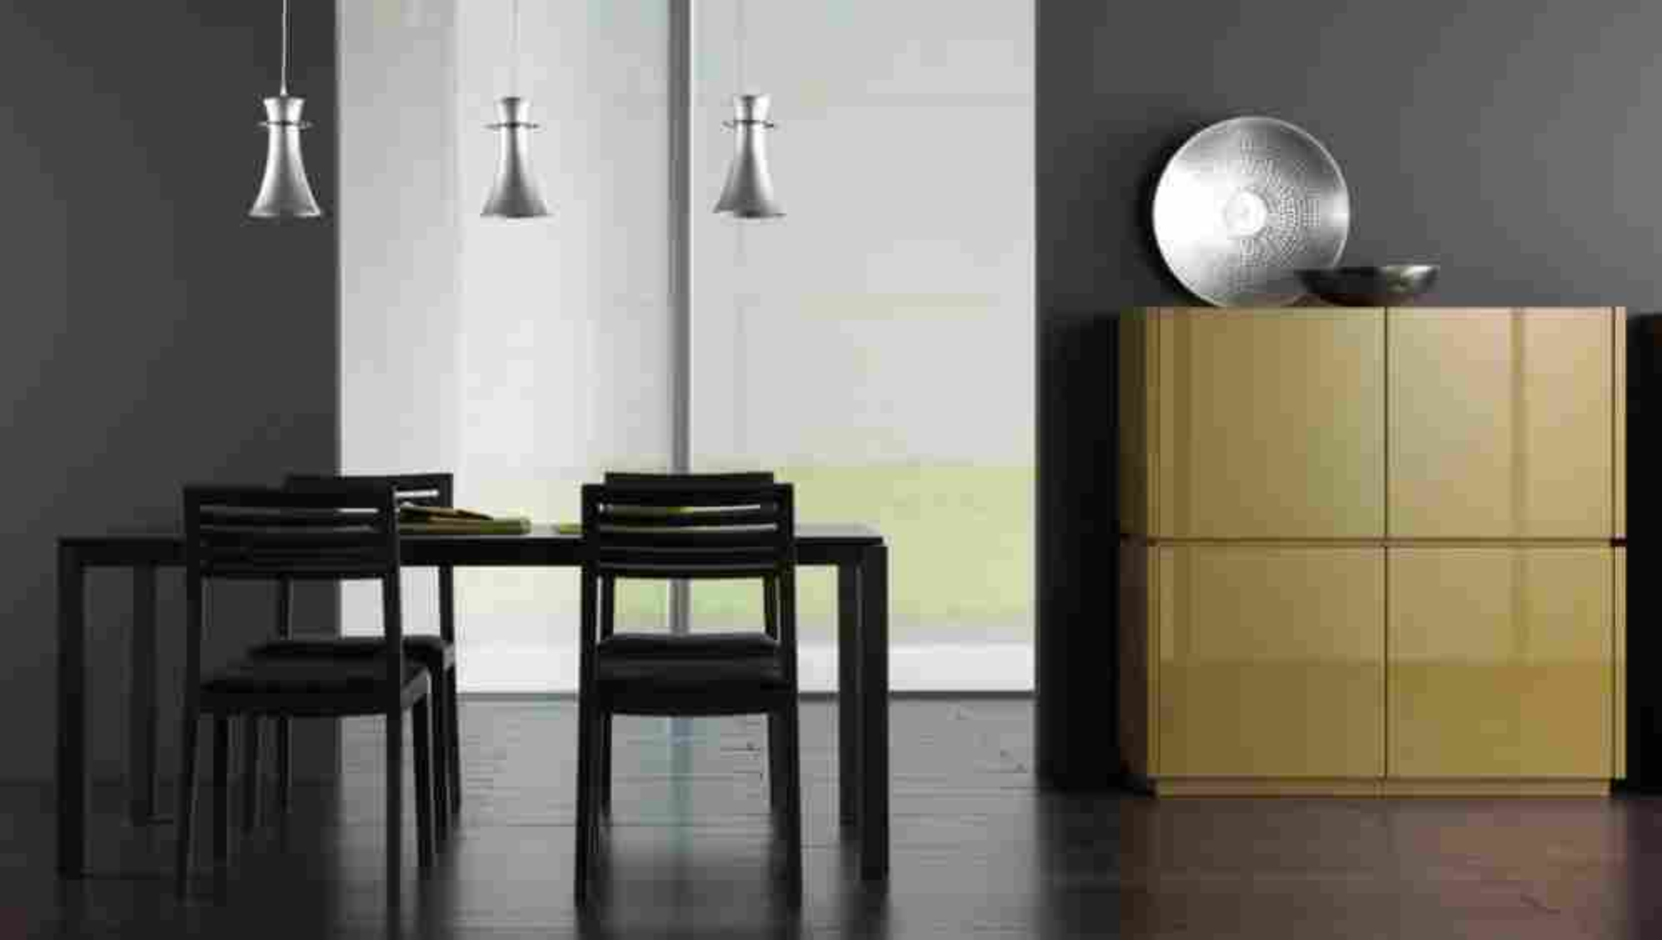
\includegraphics[width=0.8\linewidth]{muebles-azcue}}
%\end{minipage}
%
%\begin{minipage}{.3\textwidth}
%\colorbox{white}  {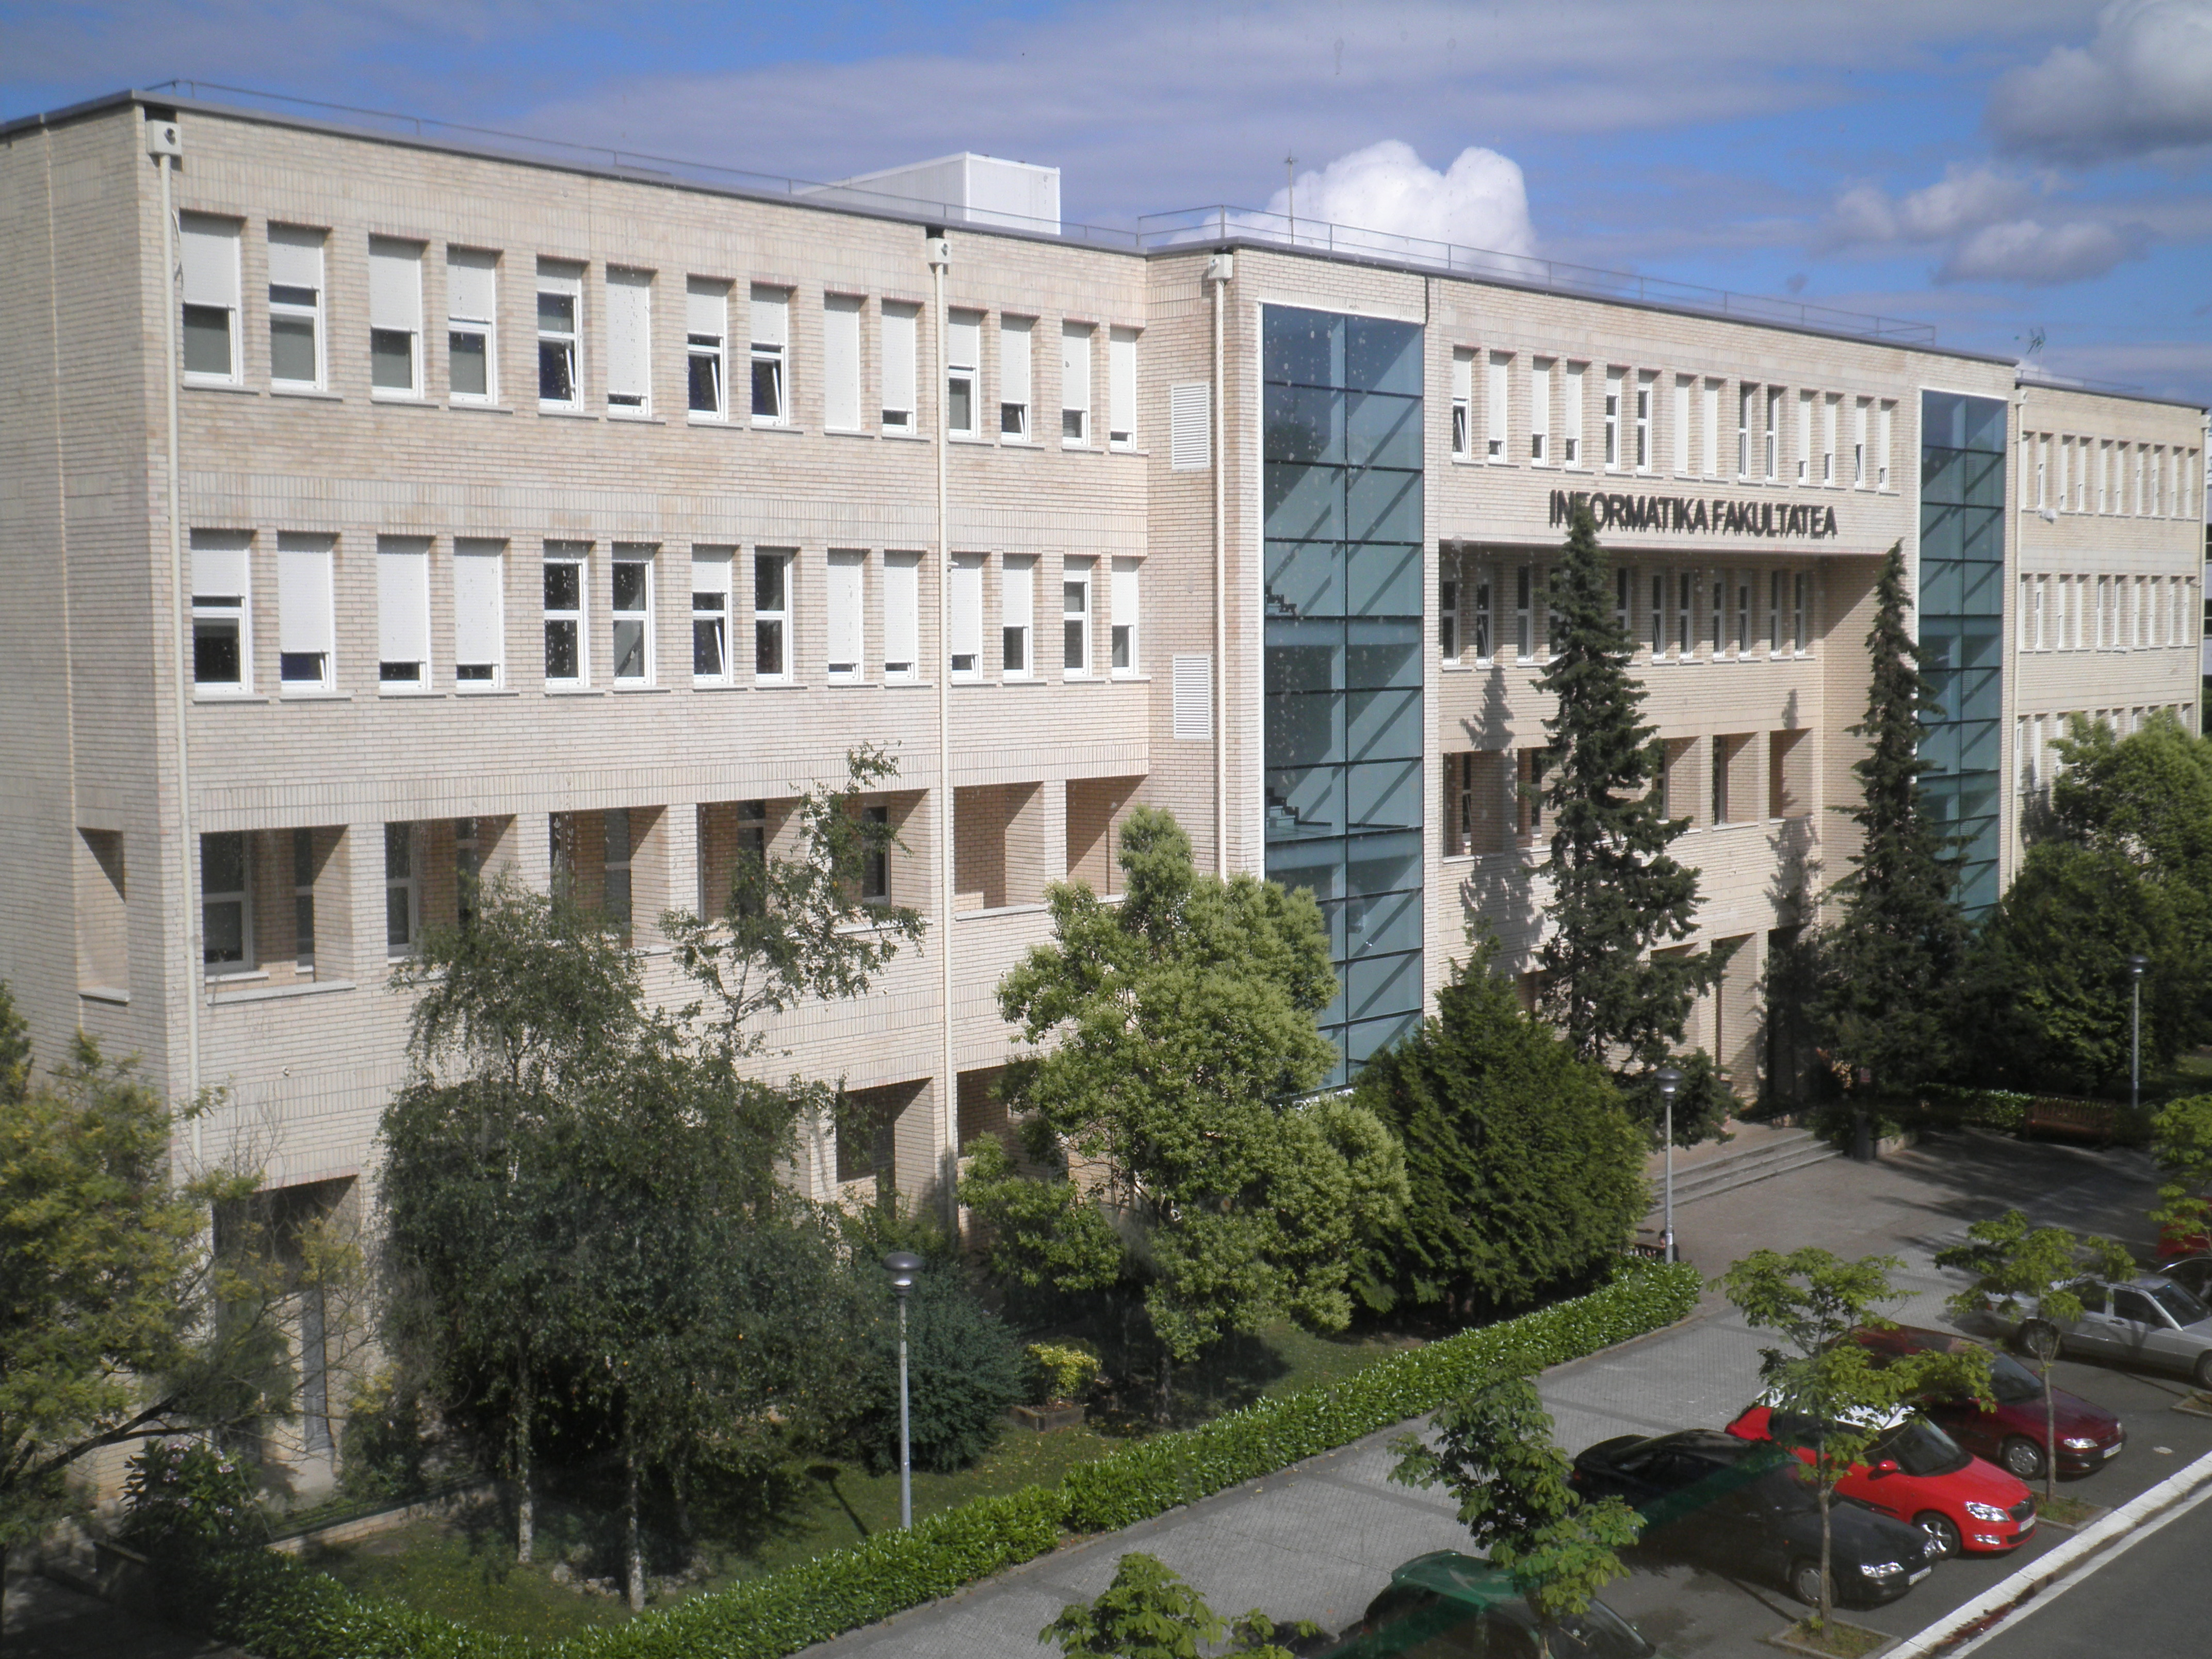
\includegraphics[width=0.8\linewidth]{Informatika_fakultatea_001}}
%\end{minipage}
%
%\begin{minipage}{.3\textwidth}
%\colorbox{white}  {\includegraphics[width=0.8\linewidth]{desertua}}
%\end{minipage}
%
%
%\end{figure}


%\end{frame}

%%%%%%%%%%%%%%%%%%%%%%%%%%%%%%%%%%%%%%%%%%%%%%%%%%%%%%%%%%%%%%%%%%%%%%%%%%%%%%%
\section[Irakaskuntzaren eta ikerketaren arloko merezimenduak]{Irakaskuntzaren eta ikerketaren arloko merezimenduak}

\begin{frame}{Irakaskuntzaren eta ikerketaren merezimenduak} 					  

%\medskip
\small 

\begin{figure}
	%
	\begin{minipage}{.4\textwidth}
		\colorbox{white}  {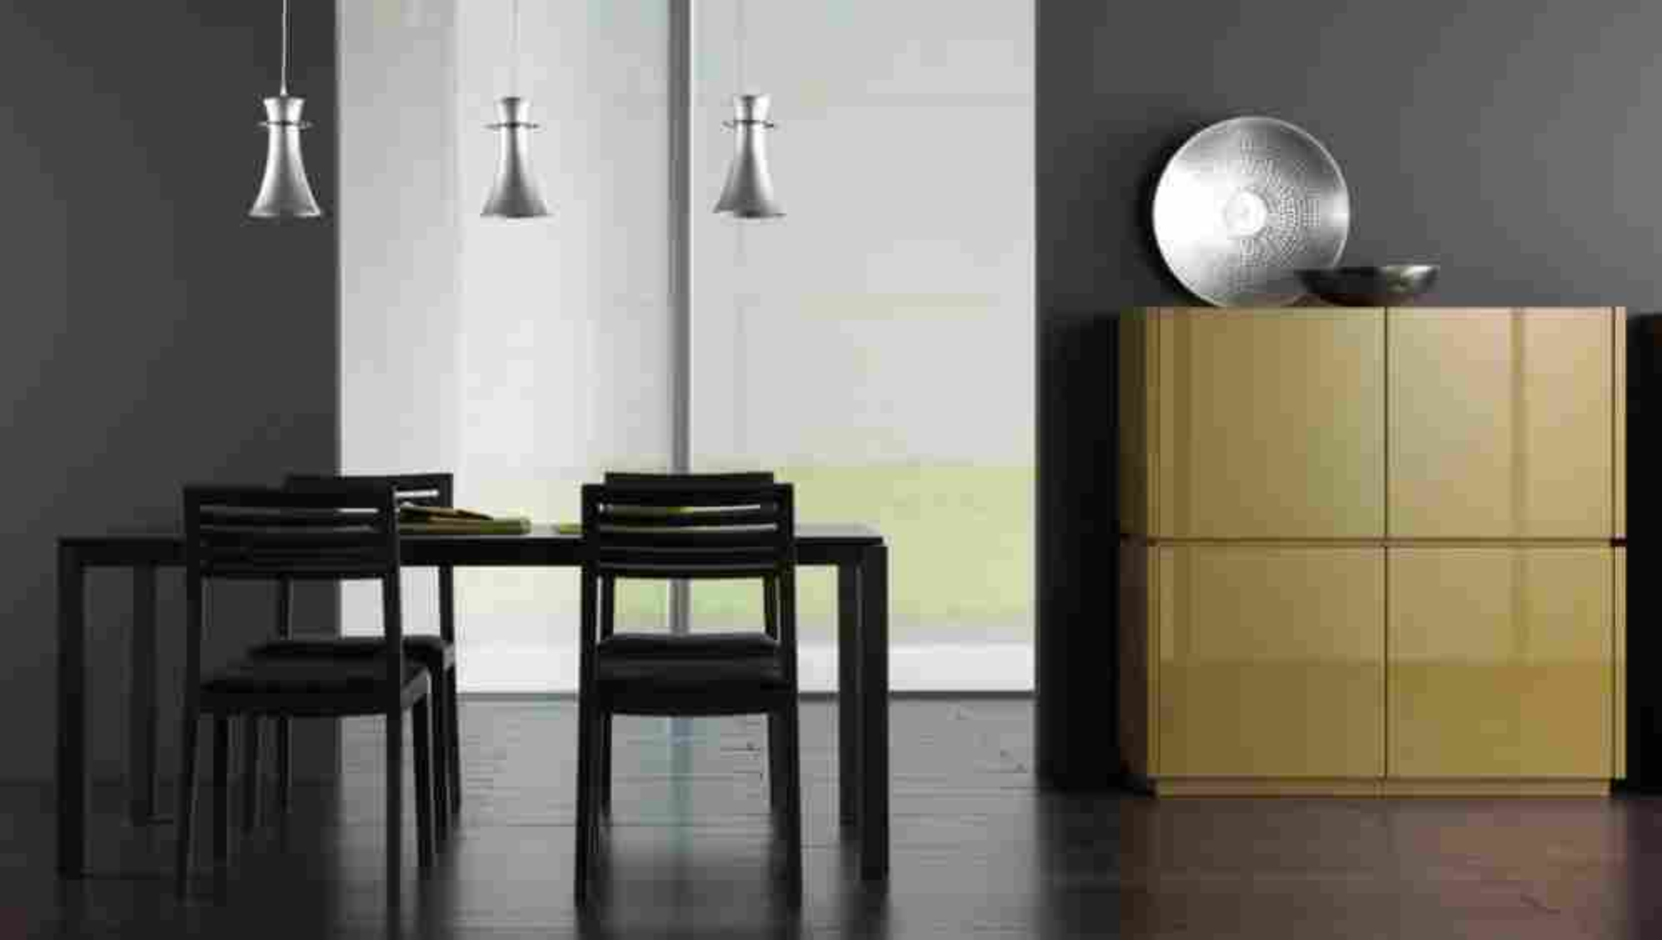
\includegraphics[width=0.8\linewidth]{muebles-azcue}}
	\end{minipage}
	%
	\begin{minipage}{.4\textwidth}
		\colorbox{white}  {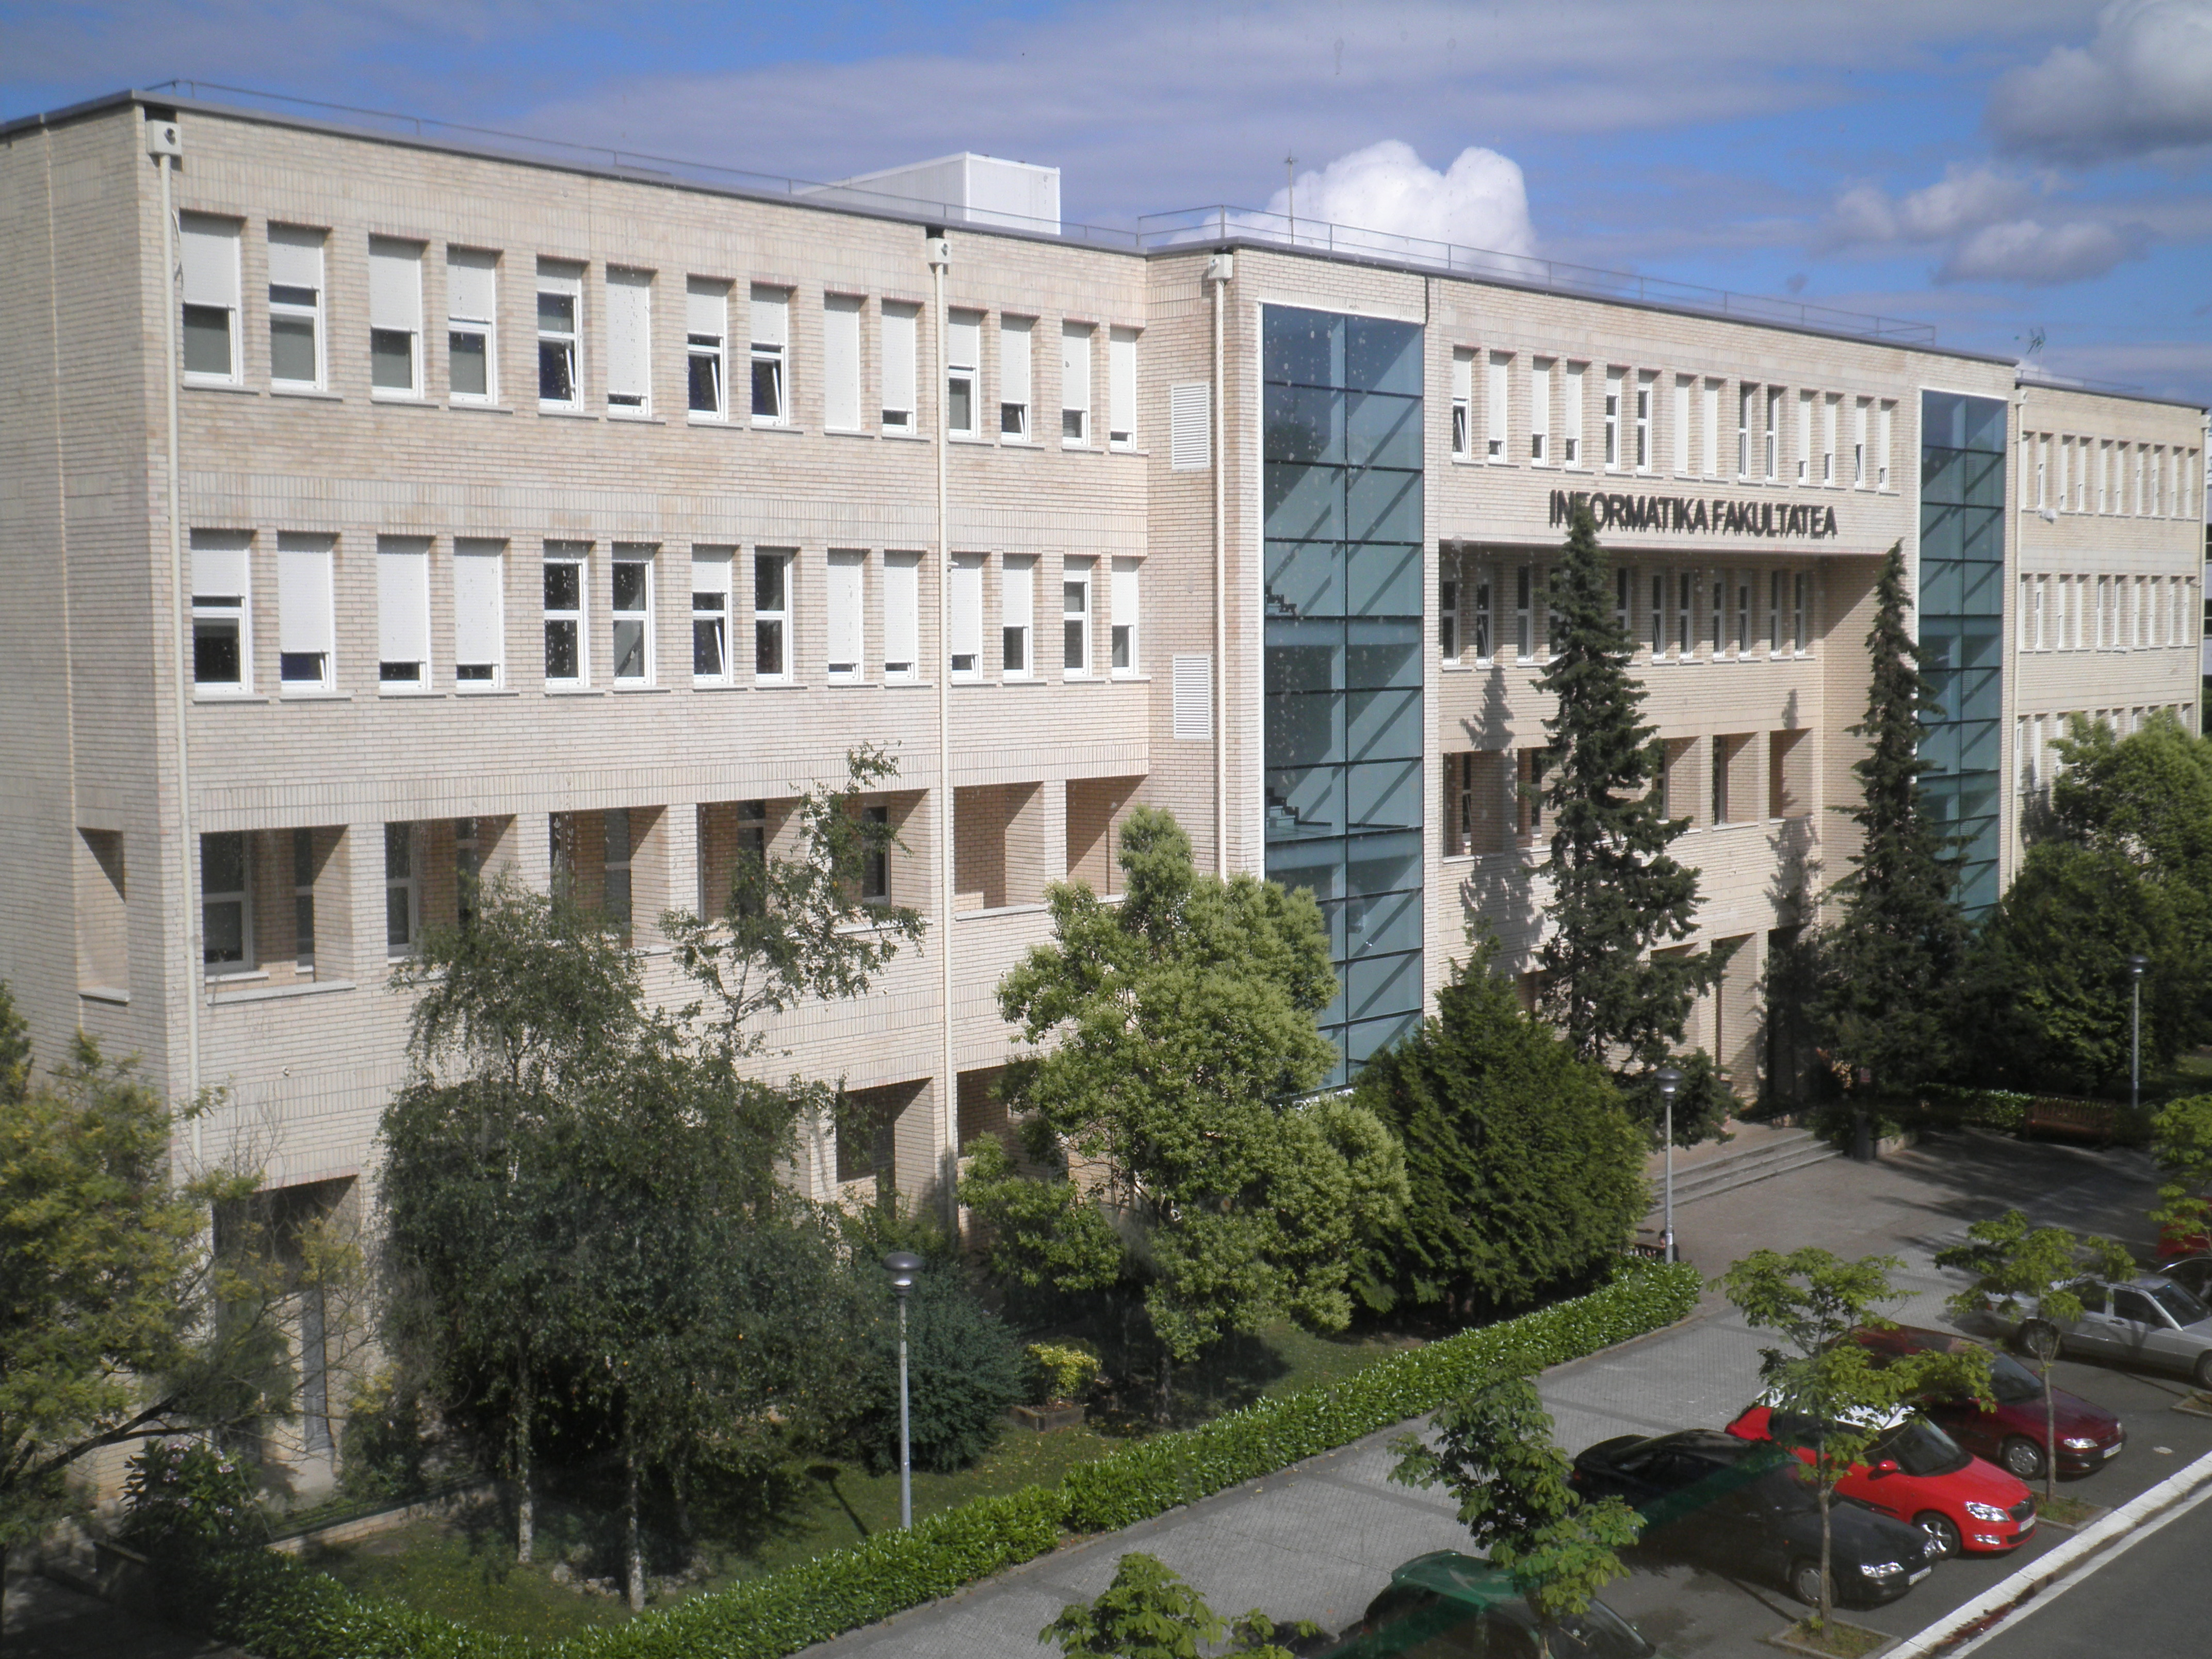
\includegraphics[width=0.8\linewidth]{Informatika_fakultatea_001}}
	\end{minipage}
	%
%	\begin{minipage}{.3\textwidth}
%		\colorbox{white}  {\includegraphics[width=0.8\linewidth]{desertua}}
%	\end{minipage}
	%
	%
\end{figure}

\begin{itemize}
%\item  \textbf{1987-1992}: Informatikan lizentziatua
%\medskip
\item \textbf{1992-2009}: Enpresa pribatua (industria sektorea)
%\begin{itemize}
%\medskip
%\item Azcue y CIA, S.A: egurrezko altzarien fabrikazioa
%\item Urteko fakturazioa ($2001-2007$) $\approx 20 \ milioi$ eurokoa
%\item Informatika saileko arduraduna 
%\end{itemize}

\medskip
\item \textbf{2009-2011}: Bizitza profesionala berreraikitzea
%\medskip
%\begin{itemize}
%\item Donostiako Nazioarteko Zinemaldia (informatika laguntzailea)
%\item Enpresa-ekimena : \textbf{informatika zerbitzuak}
%\end{itemize}

\medskip

\item \textbf{2011-2023}: Ibilbide akademikoa (UPV/EHU): 
\begin{itemize}
\medskip
\item \textbf{2011-2012}:  Irakaslea (Informatika - KZAA Saila)

\medskip
\item \textbf{2012-2013}:  KISA Masterra (Informatika Fakultatea)%KISA
% Ingeniería Computacional y Sistemas Inteligentes (ICSI)

\medskip
\item \textbf{2013-2017}:  Doktoradutza Informatika Ingeniaritza 
%\item 2017-2022:  Irakaslea (GIE - Matematika Aplikatua)

%\medskip
%\item \textbf{Akreditazioak}: Irakasle Atxiki (2019)  

%$\hspace*{2.2 cm}$ eta Irakasle Agregatua (2023)


\medskip
\item \textbf{2017-2023}:  Irakaslea (GIE - Matematika Aplikatua Saila)

\end{itemize}

\end{itemize}

\note[iten]{

Irakaskuntza eta ikerketa ibilbidekin hasi aurretik, laburki nire lan-esperientziaren bi etapak  deskribatuko ditut:

\begin{itemize}
	\item 16 urtez industria sektoreko enpresa pribatuan lan egin nuen, informatika saileko arduradun postuan.
	
	\item 2009.go krisia dela eta, enpresa utzi  eta  nire bizitza profezionala berreraikitzera behartuta nago. %2009-2011 aldi honetan Donostiako Zinemaldia lan egin eta nire enpresa-ekimena martxan jarri nuen.
	
	\item 2011an UPV/EHUko nire ibilbidea hasiko da, Informatika Fakultateko KZAA saileko urtebeteko irakasle ordezkapenarekin. Urtebeteko ordezkapena amaitzerakoan eta Ander+Joseba irakasleekin ikerketan hasia nintzelarik,  unibertsitate-irakaskuntz ibilbidean saiatzea erabakia hartu nuen.
	
%	\item Ikasturte horretan, Ander Muruaren ikertaldearekin kolaboratzen hasten naiz. 
	
	\item Hortaz, lehenengo saileko Konputazio Ingeniaritza eta Sistema Adimentsuak masterra eta ondoren Doktoradutza ikasketak egin nituen.
	
	\item 2017. urtetik aurrera, Gipuzkoako Ingeniaritza Eskolako Matematika Aplikatua Saileko irakasle ordezkapen bat betetzen ari naiz.
	
%	\item Bost urteko irakaskuntza ibilbide honetan, 2019an Irakasle atxiki  eta  2023an Irakasle agregatu akreditazioak lortu ditut
	
\end{itemize}



}

\end{frame} 


%%%%%%%%%%%%%%%%%%%%%%%%%%%%%%%%%%%%%%%%%%%%%%%%%%%%%%%%%%%%%%%%%%%%%%%%%%%%%%%

%\begin{frame}{Irakaskuntza ibilbide} 

%\vspace*{2.cm}

%\textbf{Historial académico}

%
%\begin{figure}
%\begin{minipage}{.45\textwidth}
%\colorbox{white}  {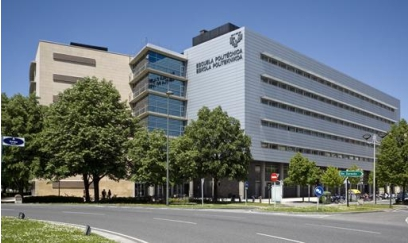
\includegraphics[width=0.8\linewidth]{Politeknikoa}}
%\end{minipage}
%
%\begin{minipage}{.45\textwidth}
%	\colorbox{white}  {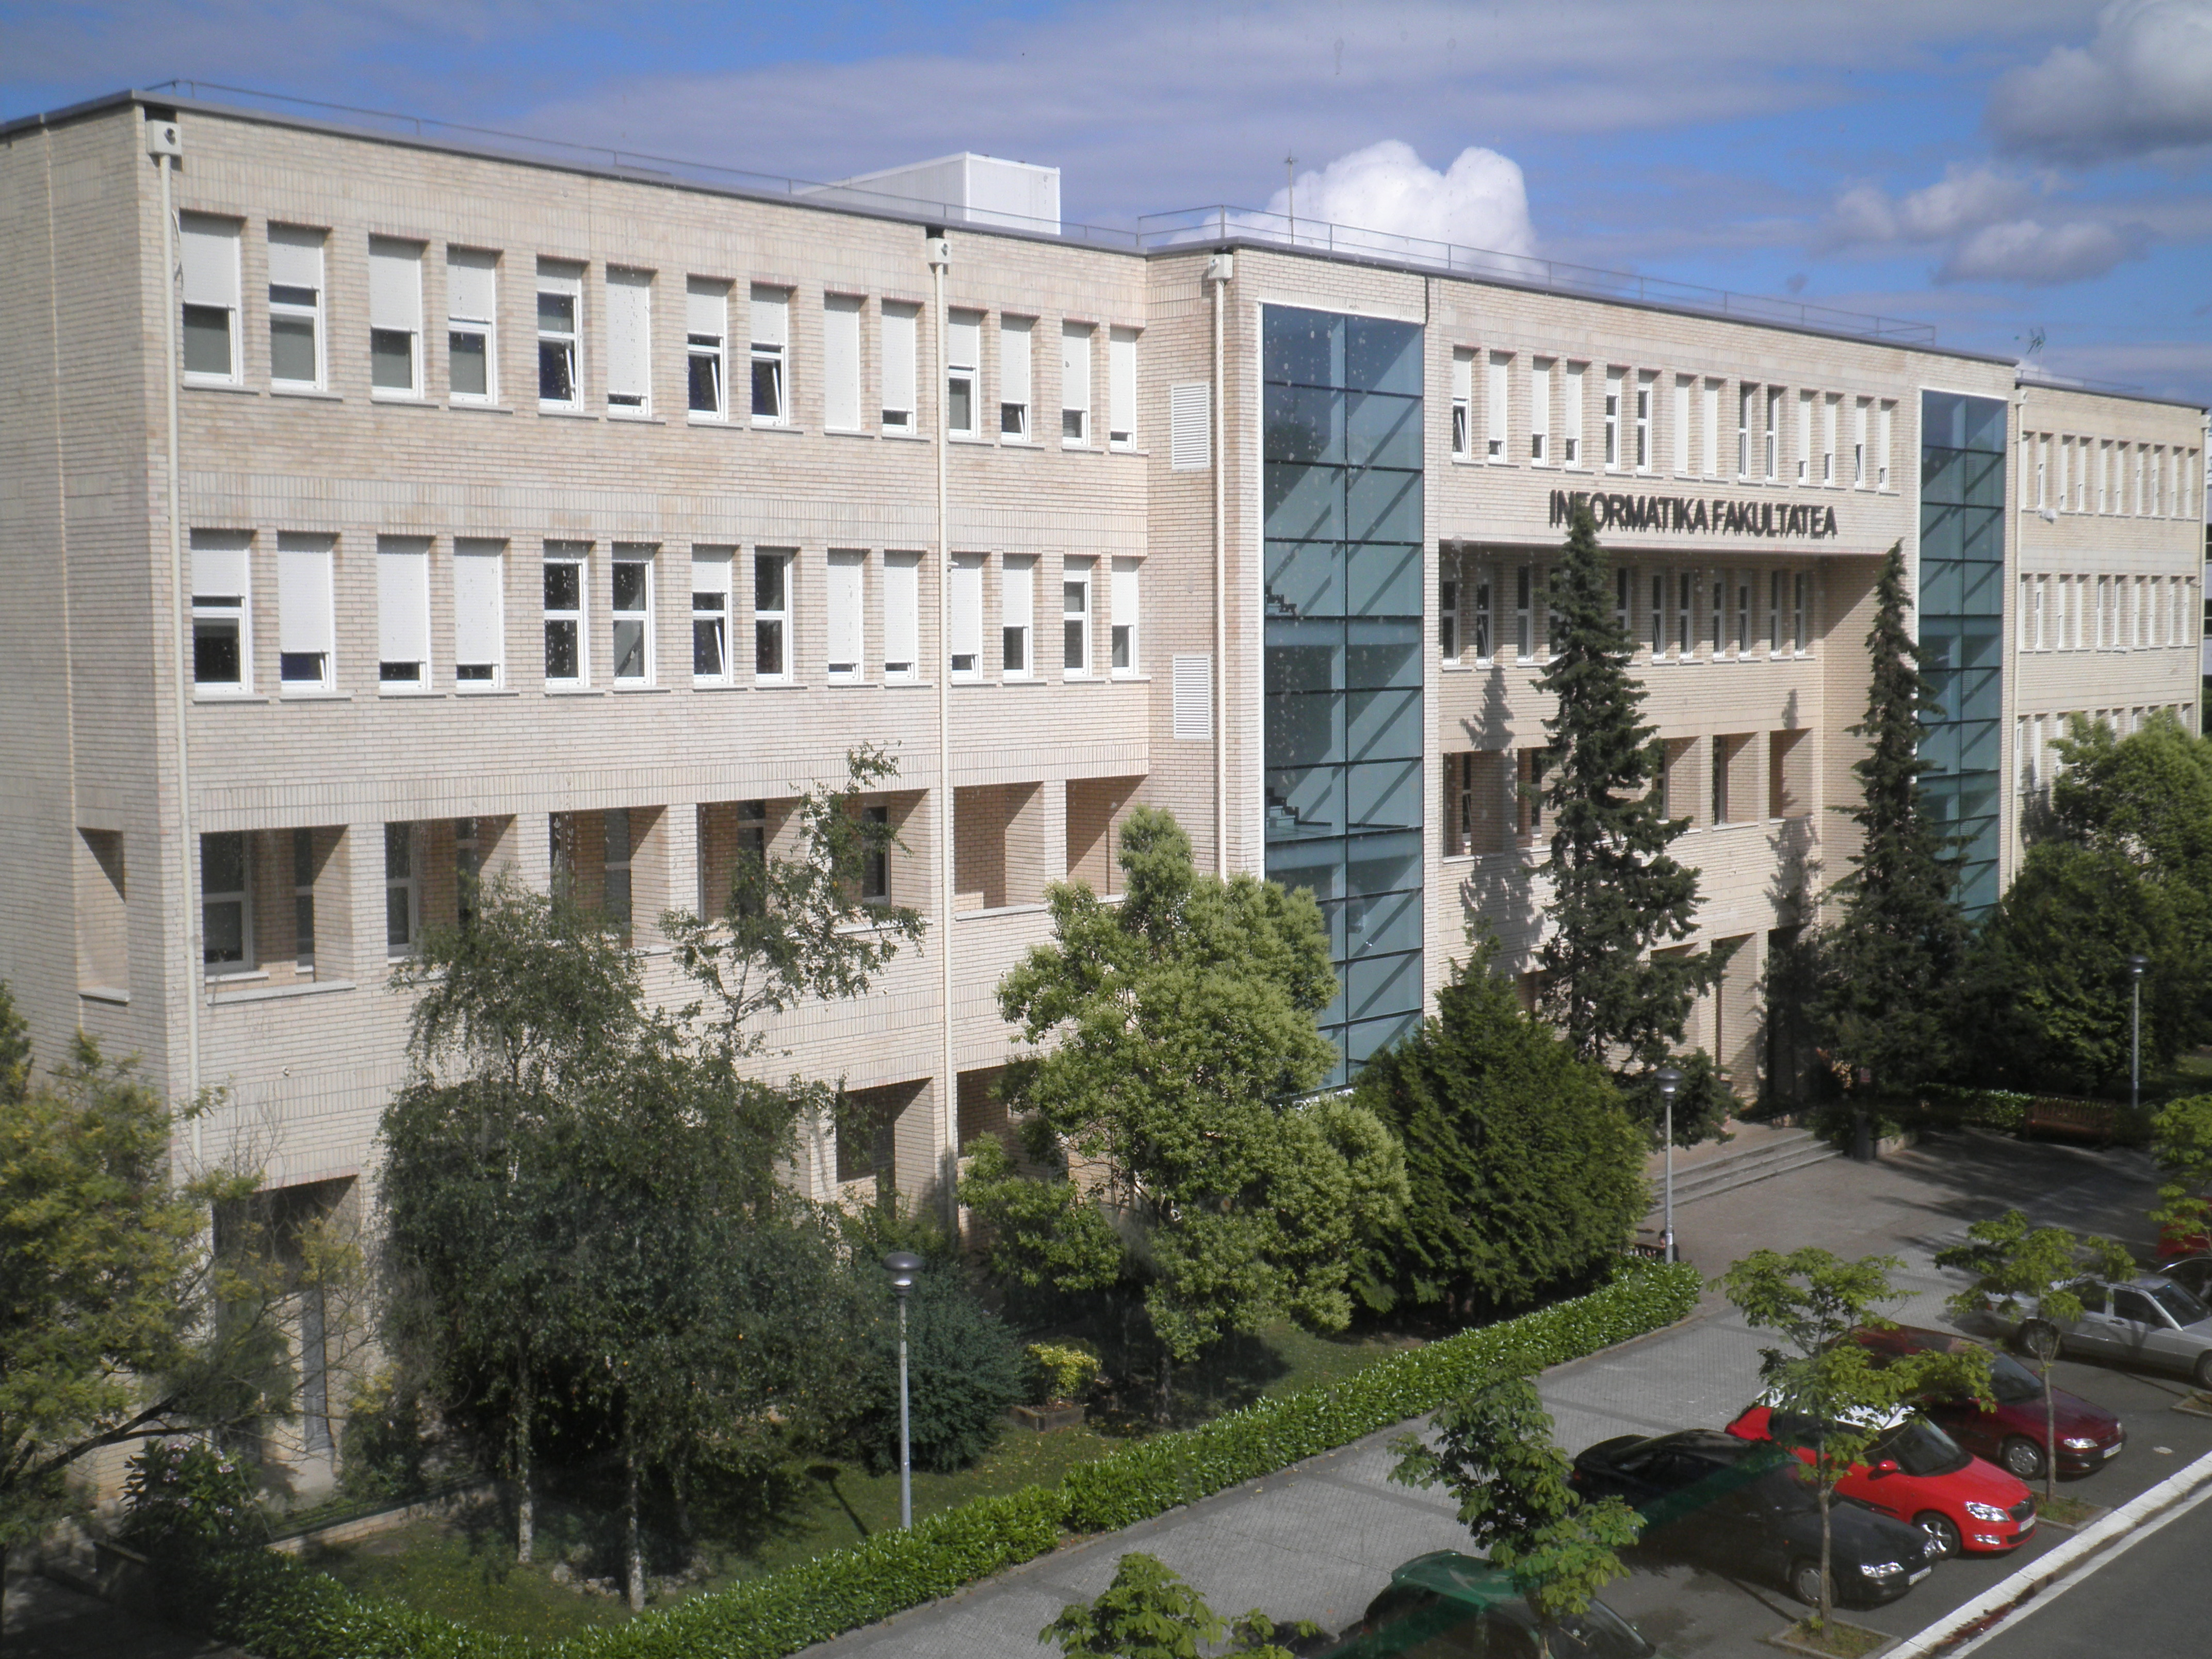
\includegraphics[width=0.8\linewidth]{Informatika_fakultatea_001}}
%\end{minipage}

%\end{figure}
%

%\end{frame}

%%%%%%%%%%%%%%%%%%%%%%%%%%%%%%%%%%%%%%%%%%%%%%%%%%%%%%%%%%%%%%%%%%%%%%%%%%%%%%%

\begin{frame}{Irakaskuntzaren merezimenduak} 

\medskip
\hspace*{3.cm} \textcolor{blue}{2011-2012 +  2017-2023}
\hspace*{2.7cm} \textcolor{blue}{Irakasle formakuntzarako urteak}

\medskip

\begin{itemize}
	
	
\item \textbf{Fakultateak}:

\begin{itemize}
\item Informatika Fakultatea: KZAA Saila 
\item Gipuzkoako Ingeniaritza Eskola: Matematika Aplikatua Saila
\end{itemize}

\medskip

\item \textbf{Graduko irakasgaiak}:

\begin{itemize}
\item Matematika Diskretua
\item Kalkulua
\item Estatistika Metodoak Ingeniaritzan
\item Aljebra

\end{itemize}

\medskip

\item \textbf{Masterreko irakasgaiak} %:(2018-2022)

\begin{itemize}
\item KISA Msterra (2018/19- 2022/23):
%Konputazio Ingeniaritza eta Sistema Adimentsuak Unibertsitate Masterra
% Computación en Ciencia e Ingeniería: simulación numérica
 
      Zientziarako eta Ingeniaritzarako konputazioa %: zenbakizko simulazioa


\end{itemize}

\end{itemize}


\note[item]{

Irakaskuntza ibilbidearen lehen urte hauek esperientzia hartzeko eta formakuntzarako ezin hobeak izan dira:


\begin{itemize}
	\medskip
	
	\item Klaseak bi zentrotan eman ditut, Informatika fakultatean eta Gipuzkoako Ingeniaritza Eskolan.
	% afinidade berdineko sailetan aritu naizela
	
	\medskip
	
	\item Bi zentrotako  Sailak Matematika Aplikatua arlokoak izanik,  
	amankomunak diren lau irakasgai hauetan aritu naiz % eta  etapa hau irakasle formakuntzarako ezin hobea izan da niretzat.
	
	\medskip
	\item Graduko ikasgai hauez gain, bost urtez   Ander Muruarekin KISA Masterreko “Zientziarako eta Ingeniaritzarako konputazioa: zenbakizko simulazio” ikasgaia partekatu dut 
	% eta beraz,  goi-mailako irakaskuntzan esperientzia hartzeko aukera izan dut. 
\end{itemize}



}

\end{frame}

%%%%%%%%%%%%%%%%%%%%%%%%%%%%%%%%%%%%%%%%%%%%%%%%%%%%%%%%%%%%%%%%%%%%%%%%%%%%%%%

\begin{frame}{Irakaskuntzaren merezimenduak} 


\medskip
\hspace*{2.cm}\textcolor{blue}{Irakaskuntzaren kalitate-adierazleak}

\medskip

\begin{itemize}
%
\small
%\begin{itemize}
%\item Campo de conocimiento de Enseñanzas Técnicas
%\end{itemize}

%\begin{itemize}
%\item Valoración global de la actividad docente: 57.09 \% (Aceptable)
%\item Periodo evaluado: del curso 2014/15 al curso 2018/19
%\end{itemize}

\medskip
\item[1)] \textbf{Ikasleen iritzien inkestak: $batezbestekoa=2.9$}
%

\bigskip

\footnotesize
\begin{center}
\begin{tabular}{ c c c c c c c c c}
 Kurtsoa & BB & &  Kurtsoa & BB & &  Kurtsoa & BB   \\ 
 \hline 
 $2011/12$ & $3.2$ &\qquad   & $2018/19$ & $2.8$ & \qquad &  $2020/21$ & $3.3$  \\  
 $2017/18$ & $2.4$ & \qquad  & $2019/20$ & $2.7$ & \qquad &  $2021/22$ & $2.9$   \\ 
 \hline   
\end{tabular}
\end{center}
%

\bigskip


\small

\item[2)] \textbf{Docentiaz Programaren balorazioa}: 57.09 \% (Onargarria)


(oso jardun laburra)

\begin{figure}
\begin{minipage}{.6\textwidth}
\colorbox{white}  {
\includegraphics[width=0.6\linewidth]{Flechas}}
\end{minipage}
\end{figure}
\end{itemize}
%
%
\normalsize
\hspace*{3.cm}\textcolor{red}{Irakaskuntza hobetzeko}\\
\hspace*{3.7cm}\textcolor{red}{5 gomendio}
%

\note[item]{

Etapa hau aberatsa izan bada ere, irakaskuntzaren kalitate-adierazleek,  hobetu beharra erakutsi didate

\medskip
\begin{itemize}
	\item Batetik irakasleen iritzien-inkesten “gogobetetze orokorra” atalean  2.9/5 batezbestekoak 
	%eta aitzakirik gabe,  balorazioa hobetu beharra ikusten dut.
	
	\medskip
	\item Bestetik, 2019. urtean Docentiaz programan lortutako 
	balorazioak. 
	
	\medskip
	\item Beraz, Docentiaz txostenean aipatzen diren irakaskuntza hobetzeko 5 gomendioei heldu diet eta orain, horietako bakoitzean egindako ahalegina komentatuko dut	
%	\medskip
%	\item Orain horietako gomedio bakoitzean egindako ahalegina banan-banan komentatuko dut
\end{itemize}



}

\end{frame}

%%%%%%%%%%%%%%%%%%%%%%%%%%%%%%%%%%%%%%%%%%%%%%%%%%%%%%%%%%%%%%%%%%%%%%%%%%%%%%%

\begin{frame}{Irakaskuntza ibilbidea} 

\medskip

%\item Tesis doctoral en \textbf{euskera} 

%Calificación: Sobresaliente Cum Laude


%\item \textbf{Encuestas positivas} 

%Cálculo(2011/2012) 3.8; Álgebra (2018/2019): 2.9

\begin{itemize}
	\item[G1)] \textbf{Irakaskuntza hobetzeko  prestakuntza jasotzea}


\bigskip
\bigskip

\small
\hspace*{0.3cm} \textcolor{blue}{UPV/EHU (HELAZ)} \hspace*{2.8cm} \textcolor{blue}{Prestakuntza teknikoa}

%\medskip
%
%
\begin{columns}
	
	\column{0.5\textwidth}
	
\begin{itemize}

	\item \textit{Zeharkako gaitasunak}
	
%	\medskip
	\item  \textit{Ebaluazio sistemak}
	
%	\medskip
	\item \textit{Irakaskuntzaren plangintza}	
	
%	\medskip
	\item \textit{Metodologia Aktiboak}
		
%	\medskip
	\item \textit{Aniztasunerako Ikuspegi Berriak} 

\end{itemize}


\medskip
\hspace*{0.5cm} \textcolor{blue}{Red Docencia Universitaria} 

\begin{itemize}
	\item Didáctica general/específica en la docencia universitaria
\end{itemize}%



	\column{0.5\textwidth}
	
\begin{itemize}
	
	\item \textit{Big Data Analitycs}
%    Barcelona Supercomputing Center
	
	\item \textit{High Performance Computing}
%	Materialen Fisika Zentroa, Donostia Intenational Physics Center
	
%	\medskip
	\item \textit{Parallel Programming}
%	Barcelona Supercomputing Center
	
%	\medskip
	\item \textit{Using Python for research}
%	HarvardX (edX)
	
%	\medskip
	\item \textit{Linear Algebra - Foundations to Frontiers}
	
%	UTAustinX (The University of Texas thorugh edX).
	
%	\medskip
%	\item \textit{Latex Dokumentu Tekniko eta Zientifikoen Edizioa}
	
	
\end{itemize}
\end{columns}


\end{itemize}


\note[item]{

Lehen gomendio honetan irakaskuntza hobetzeko prestakuntza jasotzea esaten zait.

\medskip
\begin{itemize}
	\item Batetik, UPV/EHUk irakasleei zuzendutako formazio ikastaroetan parte-hartu dut %eta  ikastaro hauei esker, UPV/EHUren IKD (Irakaskuntza Kooperatiboa eta Dinamikoa) eredua hobeto ezagutu dut
	
	%  sakontzeko baliagarria izan zait
	
	% Guztira $\approx 5$ kreditu 
	
	\medskip
	\item Bestalde, prestakuntza teknikoari lotutako beste hainbat ikastaro jaso ditut
	
%	zentro teknologikoen ikastaro presentzialak  nahiz online formakuntzarako webgune berriek  eskainitako ikastaroak baliatu ditut  prestakuntza espezializatua jasotzeko
\end{itemize}



}

\end{frame}

%%%%%%%%%%%%%%%%%%%%%%%%%%%%%%%%%%%%%%%%%%%%%%%%%%%%%%%%%%%%%%%%%%%%%%%%%%%%%%%

\begin{frame}{Irakaskuntzaren merezimenduak} 


\medskip
\small

\begin{itemize}
%	\item[G2)] \textbf{Hezkuntza berrikuntzarako ekintzak}
\item[G2)] \textbf{Hezkuntza berrikuntzarako ekintzetan parte hartzea}
%\textbf{Irakaskuntzaren arloan argitalpenak egitea }	
\small

\medskip
\begin{itemize}
\item \textbf{EuroSoTL-2019} - Irakaskuntza berrikuntzarako kongresua

%European Scholarship of Teaching and Learning Conference 

%Poster: Computational Notebooks: a powerful way to learn

%M.Antoñana, Josune Urien

%\medskip
%* Kongresuko akta liburuan: 1500 hitzetako komunikazioa

\end{itemize}


\medskip

\item[G3)] \textbf{Zabalkundean hastea}:  
	
\medskip
	
	\begin{itemize}
		\item Zientzia astea $2020 \ \& \ 2021$

	
%	\hspace*{2.cm} 2020 \hspace*{4.cm} 2021
	\begin{figure}
		%\begin{minipage}{.8\textwidth}
		%\colorbox{white}  {
\includegraphics[width=0.8\linewidth]{ZientziAstea3}}
		%  \centering \caption{\centering \tiny wikipedia}
		%\end{minipage}
		%
		\begin{minipage}{.4\textwidth}
			\colorbox{white}  {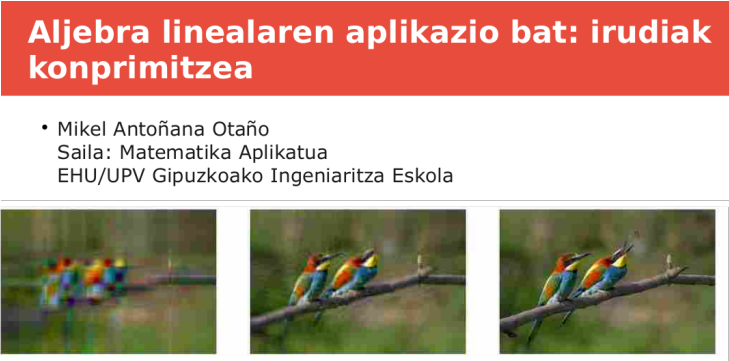
\includegraphics[width=0.8\linewidth]{ZientziaAstea2020}}
			%  \centering \caption{\centering \tiny wikipedia}
		\end{minipage}
		%
		\begin{minipage}{.4\textwidth}
			\colorbox{white}  {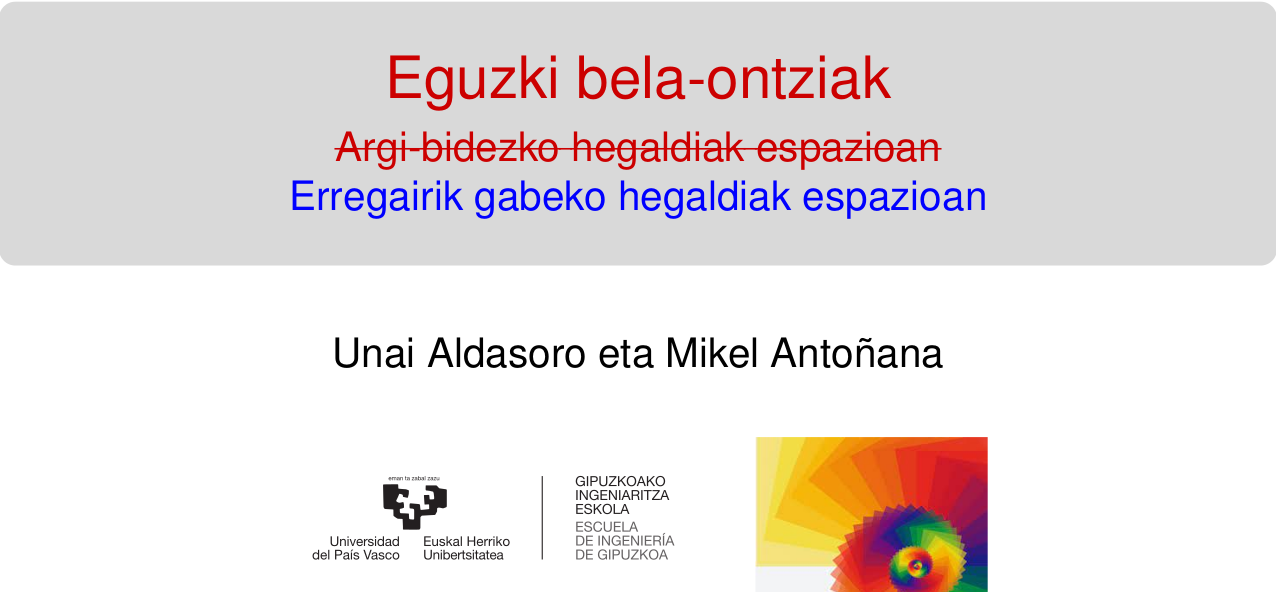
\includegraphics[width=0.8\linewidth]{ZientziaAstea2021}}
			%  \centering \caption{\centering \tiny wikipedia}
		\end{minipage}
		
		
	\end{figure}

\bigskip

     \item GIEko ikasleei zuzendutako orientazio jardunaldiak: 
     
     \begin{itemize}
     	\item Praktikak eta Enplegu jardunaldiak $2021+2022+2023$
     	\item 2021-2022 ikasturteko Harrera Eguna
     \end{itemize}
	
	\end{itemize}


\end{itemize}


\note[item]
{

\begin{itemize}
	\item \textbf{2.Gomendioa}: Hezkuntza berrikuntzarako ekintzetan parte hartzeari dagokionez, EuroSoTL-2019 izeneko Irakaskuntza berrikuntzarako   kongresuan  komunikazioa bat aurkeztu nuen 
	
	%eta kongresuko akta liburuan, 1500 hitzetako komunikazioa argitaratu genuen
	
	\medskip
	\item \textbf{3.Gomendioa}: 
	
	Zabalkundean hastearen gomendioarekin erlazionatutako bi ekintza mota burutu ditut:
	
	\medskip
	\begin{itemize}
		\item Bi urtez UPV/EHU-k antolatutako zientzia astean parte-hartu dut hitzaldi banarekin
		%
		\medskip
		\item Bestetik, GIEko ikasleen hainbat orientazio jardunaldietan parte-hartu dut:
		
%		ikasleen orientazio jardunaldi interesgarrietan parte hartu dut. Egun horretan eskolara Euskal-Herriko enpresak garrantzitsuak  hurbiltzen zaizkigu,  bere burua aurkeztu eta ikasleei  praktikak eskaintzeko.
	\end{itemize}
	
\end{itemize}

}





\end{frame}



%%%%%%%%%%%%%%%%%%%%%%%%%%%%%%%%%%%%%%%%%%%%%%%%%%%%%%%%%%%%%%%%%%%%%%%%%%%%%%%

\begin{frame}{Irakaskuntzaren merezimenduak} 

\medskip

\begin{itemize}
\item[G4)] \textbf{Irakaskuntza lidergoan parte hartzea}
%

\medskip
\begin{itemize}
\item 2020-2021 Kalkulu irakasgaiaren koordinatzailea 

Ingeniaritza Zibileko Gradua
\end{itemize}

\bigskip
\item[G5)] \textbf{Lan akademikoen zuzendaritza eta tutoretza} 

\begin{itemize}
	
\medskip
\item[1)] \textbf{MAL}:'IRKGaussLegendre.jl  Julia paketearen hobekuntza' (2022)

\medskip

%\textbf{Izenburua}: 'IRKGaussLegendre.jl  Julia paketearen hobekuntza'`

%{Defentsa data}: 2022-07-19
	
%\medskip

\item[2)] \textbf{GRAL}: 'Espazio ontzi baten ilargira joan etorriko ibilbidearen zenbakizko simulazioa'
(2022)
%\medskip

%\textbf{Izenburua}:'Espazio ontzi baten ilargira joan etorriko ibilbidearen zenbakizko simulazioa'
%

%{Defentsa data}: 2022-Uztaila




\end{itemize}

\end{itemize}


\note[item]
{
	
	\begin{itemize}
		\item \textbf{4.gomendioa}. Irakaskuntza lidergoari dagokion jardueretan parte hartzea 
		
		\medskip
		Ingeniaritza Zibileko Graduan, Kalkulua ikasgaiaren koordinatzailea izateko aukera izan dut
		
		\medskip
		\item \textbf{5.gomendioa}.Lan akademikoen zuzendaritza eta tutoretza
		
		\medskip
		 2022. urtean defendatutako ondorengo lanak zuzendu ditut:
		 
		 \begin{itemize}
		 	\item GRAL: Espazio ontzi baten ilargira joan etorriko ibilbidearen zenbakizko simulazioa
		 	
		 	\item MAL:  IRKGaussLegendre.jl  Julia paketearen hobekuntza
		 \end{itemize}
		 
	\end{itemize}
	
	
	
}

\end{frame}



%%%%%%%%%%%%%%%%%%%%%%%%%%%%%%%%%%%%%%%%%%%%%%%%%%%%%%%%%%%%%%%%%%%%%%%%%%%%%%%

\begin{frame}{Irakaskuntzaren merezimenduak} 
	
\medskip


\textbf{Akreditazioak}
\begin{itemize}
	
	\medskip
	\item \textbf{2019ko maiatza-UNIBASQ} Irakasle Atxikia 
	
	Irakaskuntza teknikoak arloan 
	
	\medskip
	\item \textbf{2023ko urtarrila-ANECA}: Profesor Contratado Doctor
	
	
	\medskip
	\item \textbf{2023ko maiatza-UNIBASQ}: Irakasle Agregatua 

    Zientzia Esperimentalak arloan
    
\end{itemize}



\note{
	
	
	Neurri batean behintzat, lan honen errekonozimendua lortutako akreditazioetan gauzatu da:
	
	\medskip
	\begin{itemize}
		\item 2019ko maiatzan Irakasle atxiki figuran aldeko ebaluazioa
		
	    \item 2023ko urtarrilen Profesor Contratado Doctor figuran aldeko ebaluazioa
	    
	    \item 2023ko maiatzan Irakasle agregatu figuran aldeko ebaluazioa
	\end{itemize}
	
	
	
	
}


\end{frame}

%%%%%%%%%%%%%%%%%%%%%%%%%%%%%%%%%%%%%%%%%%%%%%%%%%%%%%%%%%%%%%%%%%%%%%%%%%%%%%%

\begin{frame}[fragile]{Ikerketaren merezimenduak} 					  

%\medskip

%\textbf{Historial de investigación}


%KZAA Sailaren ikerketa arloak

%\hspace*{2.5cm} \textcolor{blue}{Konputazio zientzia}

%\centering \textcolor{blue}{Konputazio zientzia}

\small

\centering EDAk modelizatutako problemen zenbakizko integraziorako metodo aurreratuen analisia eta inplementazioa.

\medskip



%\begin{figure}
%	\begin{minipage}{.4\textwidth}
%		\colorbox{white}  {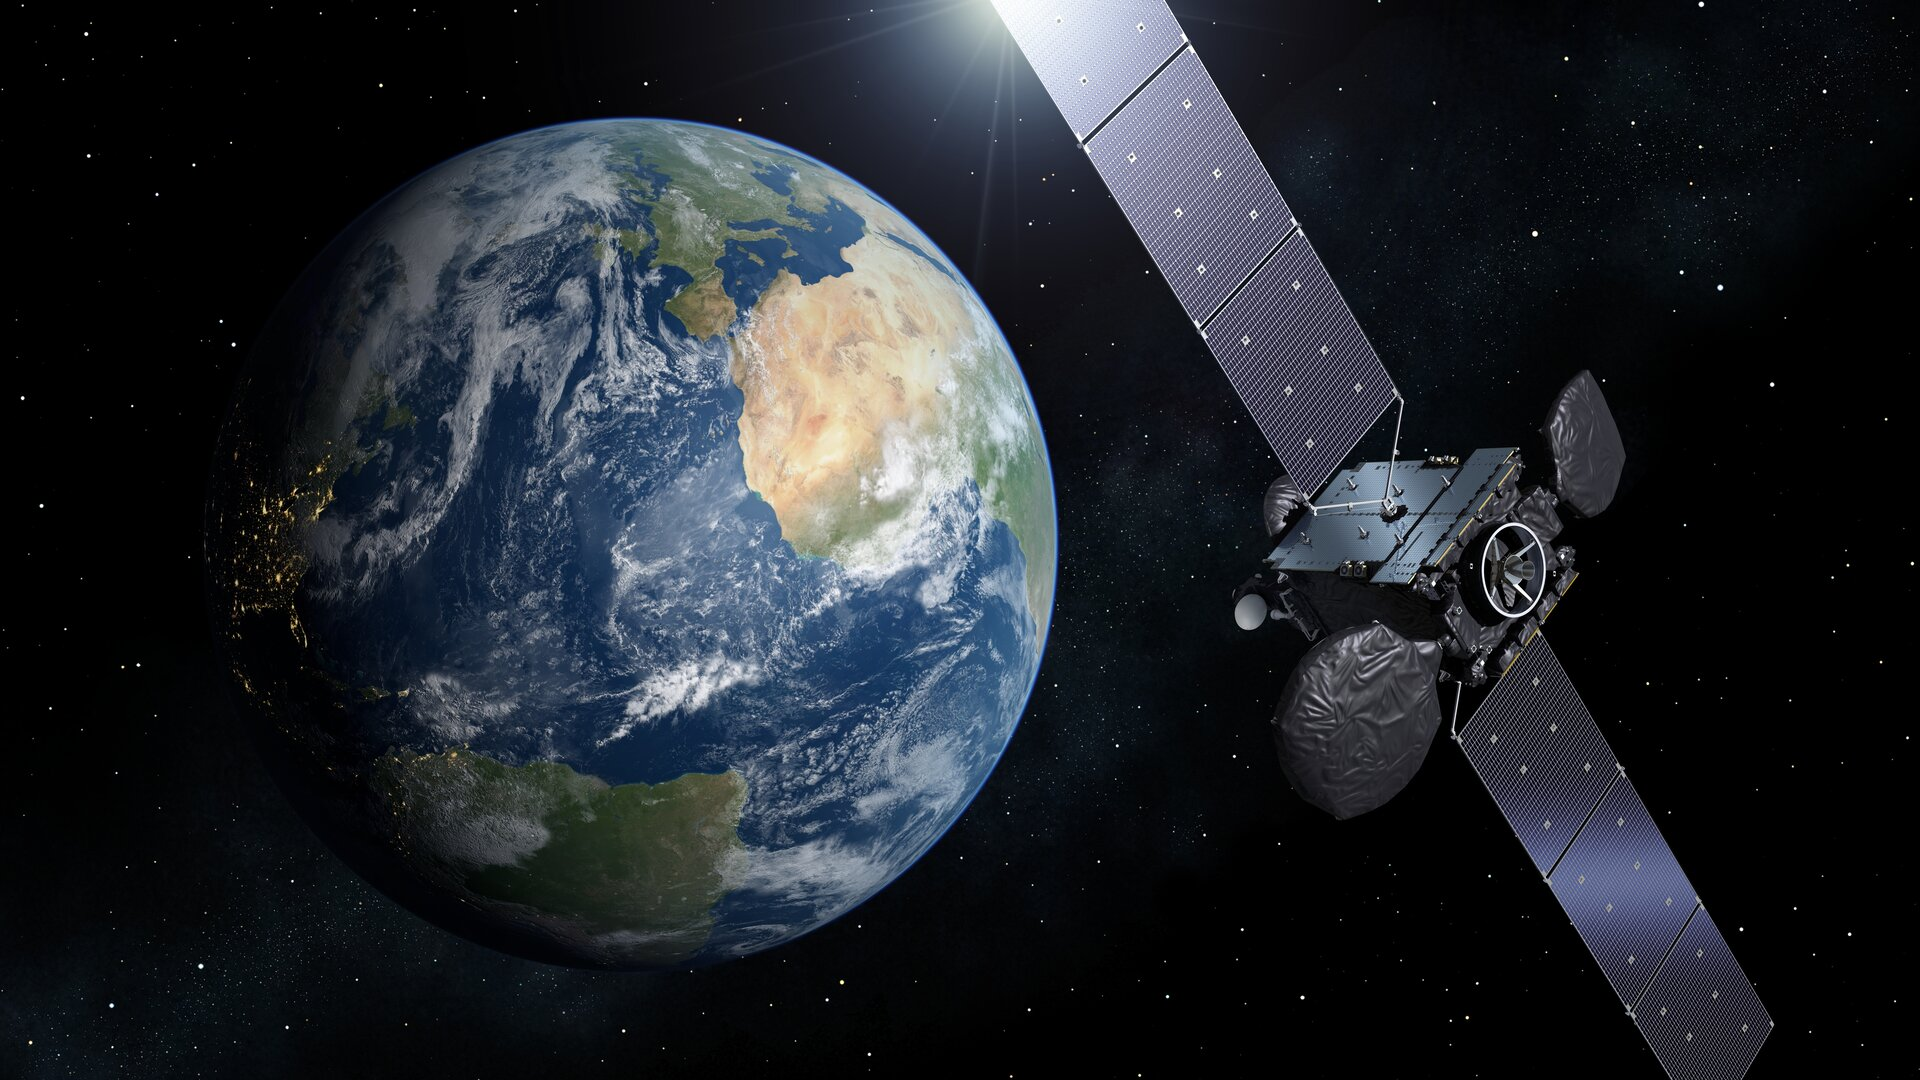
\includegraphics[width=0.8\linewidth]{SmallGEO_Hispasat_36W-1_pillars}}
%	\end{minipage}
%
%	\begin{minipage}{.4\textwidth}
%	\colorbox{white}  {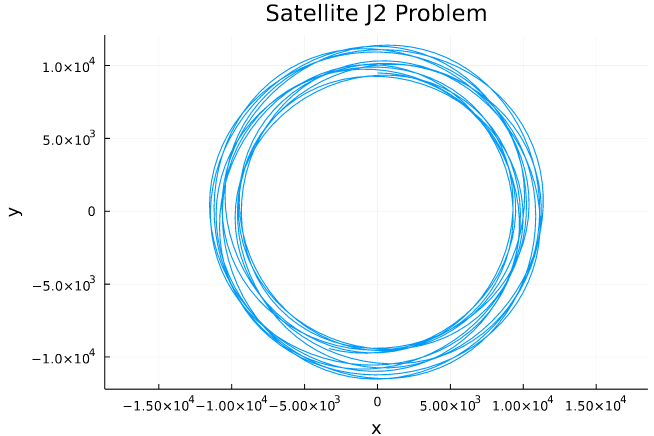
\includegraphics[width=0.8\linewidth]{J2 VOP Problem}}
 %   \end{minipage}
%\end{figure}
%
%
%
%\medskip
%
\begin{columns}
%	
\column{0.5\textwidth}
%
\tiny
%

\centering
\begin{minipage}{.8\textwidth}
	\colorbox{white} 
	 {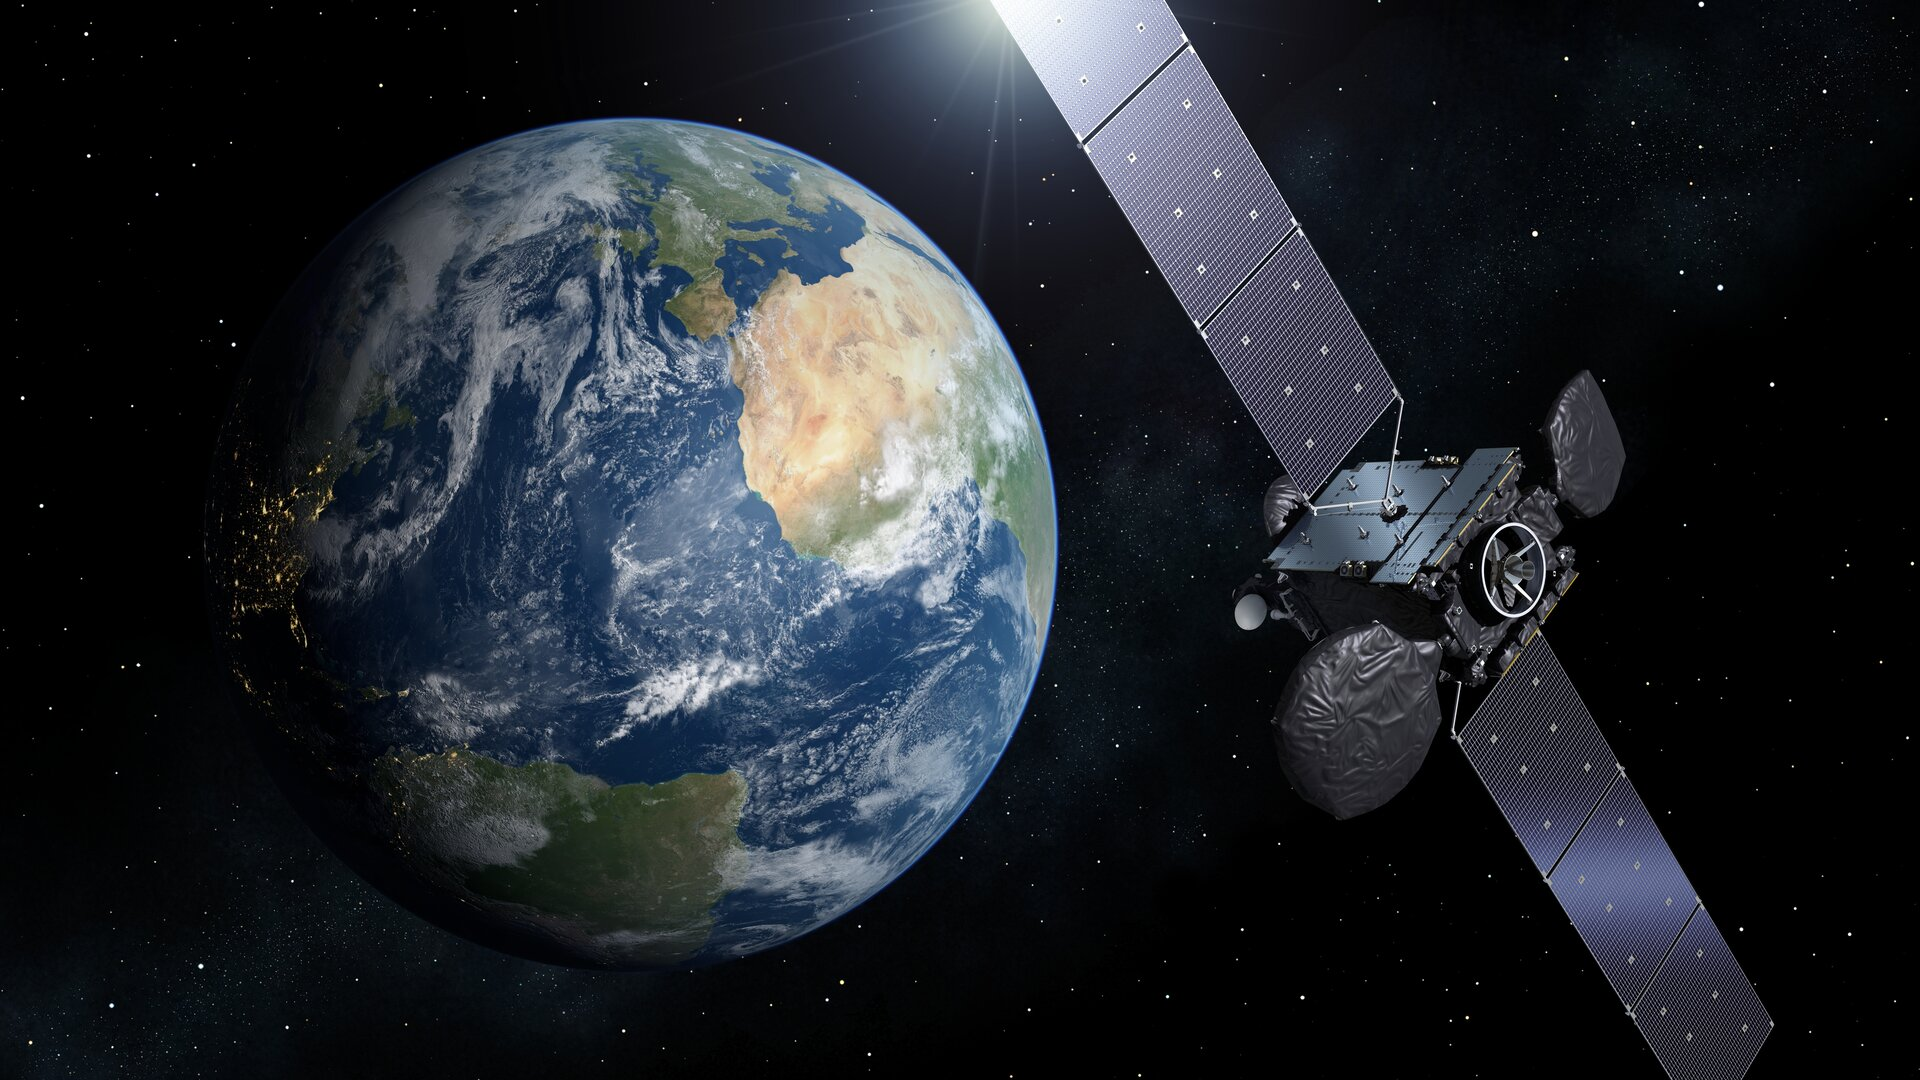
\includegraphics[width=0.8\linewidth]{SmallGEO_Hispasat_36W-1_pillars}}
\end{minipage}

%
\begin{align*}
&\frac{d^2}{dt^2} 
\left(
\begin{matrix}
%x \\ y \\ z \\v_x \\ v_y\\ v_z
x \\ y \\ z 
\end{matrix}
\right)
=
\left(
\begin{matrix}
%v_x\\
%v_y\\
%v_z\\
\displaystyle -\mu \frac{x}{r^3} \left(1 + \frac{\epsilon R^2}{r^2}\, F \right)\\ 
\displaystyle -\mu \frac{y}{r^3} \left(1 + \frac{\epsilon R^2}{r^2}\, F \right)\\ 
\displaystyle-\mu \frac{z}{r^3} \left(1 + \frac{\epsilon R^2}{r^2}\, G \right)
\end{matrix}
\right) \\
&\text{non} \\
& r=\sqrt{x^2+y^2+z^2}, \\
& F = \frac{3}{2} -  \frac{15z^2}{2r^2}, \quad
G = \frac{9}{2} - \frac{15z^2}{2r^2}
\end{align*}
%
%
%
\column{0.4\textwidth}
%
%

\centering
\begin{minipage}{0.8\textwidth}
	\colorbox{white}  {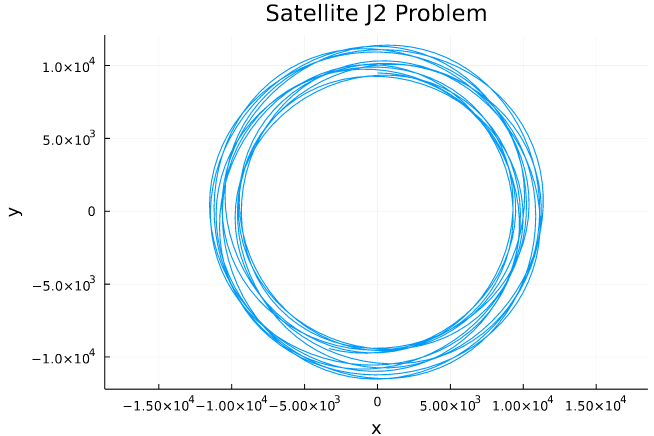
\includegraphics[width=0.8\linewidth]{J2 VOP Problem}}
\end{minipage}

%
\begin{code}
function J2ODE!(du,u,p,t)
	r2 = x^2+y^2+z^2
	r = sqrt(r2)
	aux1 = -μ/(r*r2)
	F = 1.5 - 7.5*(z/r)^2
	G =  3 + F
	aux2 = ϵ*R^2/r2
	aux3 = aux1*(1+aux2*F)
	aux4 = aux1*(1+aux2*G)
	du[4]=aux3*x
	du[5]=aux3*y
	du[6]=aux4*z
	return nothing
end
\end{code}

\end{columns}

	%




\note
{
	
\begin{itemize}
%	\item Une honetan ikerkuntza merituen azalpenetara salto egingo dut.
	
	\medskip
	\item Ikerketa merezimenduen azalpenetara salto eginez, lehenik gure ikerketa EDAk modelizatutako problemen zenbakizko integraziorako metodo aurreratuen analisia eta inplementazioaren arloan kokatzen dela esanez hasiko naiz
	
	
%	\medskip	
%	\item gure ikerketa Konputazio zientzia arloan kokatzen dela  eta hau bat datorrela KZAAren sailaren ikerkuntza eta ezagutza arloekin aipatu nahi dut
	
	\medskip
	\item Honek inplikatzen du, konputazio zientziaren definizioarekin bat eginez: gure ikerketan modelizazio, matematika, zenbakizko metodoak, eta programazioa konbinatzen ditugula
	
	  
\end{itemize}

 


}




\end{frame}

%%%%%%%%%%%%%%%%%%%%%%%%%%%%%%%%%%%%%%%%%%%%%%%%%%%%%%%%%%%%%%%%%%%%%%%%%%%%%%%

\begin{frame}{Ikerketaren merezimenduak} 					  

\medskip
\small

\begin{itemize}
\item \textbf{MATHMODE}  (Group on Applied Mathematical Modeling, Statistics, and Optimization) taldeko kidea
%

\begin{itemize}
\item Eusko Jaularitzak talde kontsolidatua izendatua (2022-2025)
\item BCAMek koordinatua
\end{itemize}
%
\medskip
\item 
\textbf{Azpitaldea}: zenbakizko metodo aurreratuak
%
%
\medskip

%\begin{displayquote}
%EDAk modelizatutako problemen zenbakizko integraziorako metodo aurreratuen analisia eta inplementazioa.
%\end{displayquote}

\small
\begin{itemize}
\item \textbf{Ander Murua}. Informatika Fakultatea-KZAA %Sailan irakasle osoa
%
\item \textbf{Joseba Makazaga}. Informatika Fakultatea-KZAA% Sailan irakasle agregatua
%
\item \textbf{Elisabete Alberdi}. BIE-Matematika Aplikatua %Sailan irakasle agregatua

 
%
%\item \textbf{Ainhoa Iñiguez Goizueta}. Profesora adjunta en el departamento de Matemática Aplicada de la Escuela de Ingeniería de Bilbao de la UPV/EHU
%
\item \textbf{Mikel Antoñana Otaño}. GIE-Matematika Aplikatua %Sailan irakaslea
\end{itemize}

\end{itemize}


\note[item]
{

\begin{itemize}
\item MATHMODE taldeko kidea naiz, Eusko Jaularitzak talde kontsolidatua izendatua (2022-2025) eta BCAMek koordinatua
%

\medskip
\item Zenbakizko metodo aurreratuak aztergai dugun azpitaldea, Matematikariak eta informatikariak osatzen dugu:

Ander Murua, Joseba Makazaga, Eli Alberdi eta ni neu.


%\medskip
%\item EDAk modelizatutako problemen zenbakizko integraziorako metodo aurreratuen analisia eta inplementazioa.

\end{itemize}


}

\end{frame}

%%%%%%%%%%%%%%%%%%%%%%%%%%%%%%%%%%%%%%%%%%%%%%%%%%%%%%%%%%%%%%%%%%%%%%%%%%%%%%%

\begin{frame}{Ikerketaren merezimenduak} 					  

\medskip

\begin{itemize}

\item \textbf{Ikerketa proiektuen zerrenda}

\medskip
\small
\begin{itemize}
\item \textbf{MINECOG/P37} (Estatukoa): 2011-2013

\textit{Aspectos Algebraicos y Computacionales en integración Geométrica}

\medskip
\item \textbf{IT649-113} (Autonomikoa):2013-2018

\textit{Modelización Matemática, Simulación y Aplicaciones Industriales}

\medskip
\item \textbf{MINECOR1616/P94} (Estatukoa): 2017-2019

\textit{Imágenes Electromagnéticas del Subsuelo Terrestre utilizando Métodos Avanzados de Garlekin}

\medskip
\item \textbf{IT1294-19} (Autonomikoa): 2019-2021  

\textit{Multiscale Inversion of Porous Rock Physics using High-Performance Simulators. Bridging the Gap Mathematics and Geophysics}

\medskip
\item \textbf{PID2019-104927GB-C22} (Estatukoa): 2020-2023

\textit{Geometric Numerical Integrators For Quantum Problems, Celestial Mechanics and Monte Carlo simulations} 

\end{itemize}

\end{itemize}


\note[item]{
%
Talde honen eskutik, urte hauetako ikerketa proiektuak zerrendatzen ditut:
%

\medskip
\begin{itemize}
\item Ikerketa autonomikoak eta estatukoak
%
\medskip
\item Nire ibilbidean zehar proiektuen babesa izan dudala
\end{itemize}



}


\end{frame}


%%%%%%%%%%%%%%%%%%%%%%%%%%%%%%%%%%%%%%%%%%%%%%%%%%%%%%%%%%%%%%%%%%%%%%%%%%%%%%%

\begin{frame}{Ikerketaren merezimenduak} 
	
	\medskip
	
\begin{itemize}
	\item 	\textbf{Artikuluen argitalpenak}
	
    \medskip
    
	\small

\begin{itemize}
	\item \textcolor{blue}{Kopurua}: 6
	
	\medskip
	\item \textcolor{blue}{Sailkapena}:
	%
%	\begin{itemize}
%		\item 	 
		$Q_1=4 \qquad Q_2=1 \qquad Q_3=1$
%	\end{itemize}

%	\medskip
%	\item \textcolor{blue}{Zita kopurua}: $25$ 
	
	\medskip
	\item \textcolor{blue}{Aldizkariak}:
	%	
	\begin{itemize}
		\item Numerical Algorithms
		\item Journal of Scientific Computing
		\item SIAM Journal on Applied Dynamical Systems
		\item International Journal of Computer Mathematics
		\item Celestial Mechanics and Dynamical Astronomy
	\end{itemize}
	
\end{itemize}

\medskip

\item \textbf{Software argitalpenak}

\medskip
\begin{itemize}
	\item \textcolor{blue}{Software Zientifikoa (SciML)}: IRKGaussLegendre.jl paketea (Julia)
\end{itemize}

\end{itemize}


\note[item]{

Proiektu hauei esker lortutako emaitzekin oso pozik nago:

\medskip

\begin{itemize}
\item Guztira 6 artikulu burutu ditugu eta guztiak, goi-mailako aldizkarietan argitaratuak

\medskip
\item Bestalde,  gure  inplementazio bat Software Zientifikoa biltzen duen SciML erakundearen bilgunean argitaratu  dugula nabarmendu beharra dago.

\medskip
\item Orain emaitza hauei buruzko zehaztapen batzuk emango ditut

\end{itemize}



}

\end{frame}

%%%%%%%%%%%%%%%%%%%%%%%%%%%%%%%%%%%%%%%%%%%%%%%%%%%%%%%%%%%%%%%%%%%%%%%%%%%%%%%

\begin{frame}{Ikerketaren merezimenduak} 

\medskip
\textbf{Artikuluak (I)}: \textcolor{blue}{IRKGL metodo inplizitu eta sinplektikoak}

\medskip
%Matematika aplikatuaren arloan Q1 gisa sailkatutako aldizkaritan:
%Revistas clasificadas como Q1 en el área de la Matemática Aplicada
\medskip
\begin{itemize}
%\medskip
\small
\item[1)] \textbf{\textit{Reducing and monitoring round-off error propagation for symplectic implicit Runge-Kutta schemes}}. M. Antoñana, J. Makazaga, A. Murua. Numerical Algorithms (2017)

\medskip
\item[2)] \textbf{\textit{Efficient implementation of symplectic implicit Runge-Kutta schemes with simplified Newton iterations}}. M. Antoñana, J. Makazaga, A. Murua. Numerical Algorithms (2017)

\medskip
\item[3)] \textbf{\textit{New integration methods for perturbed ODEs based on symplectic implicit Runge- Kutta schemes with application to solar system simulations}}. M. Antoñana, J. Makazaga, A. Murua.

Journal of Scientific Computing (2018)

\medskip

\item[4)] \textbf{\textit{An implicit symplectic solver for high-precision long term  integrations of the Solar System}}. M. Antoñana, E. Alberdi, J. Makazaga, A. Murua.  Celestial Mechanics and Dynamical Astronomy (2022) 


\end{itemize}
%

\note[item]{


\begin{itemize}
\item Artikulu talde hau,  Runge-Kutta Gauss-Legendre  metodo Inplizitu eta sinplektikoen analisi eta garapenari lortua dago. Metodo hauek, problema kontserbakorren epe luzeko eta doitasun altuko zenbakizko integrazioetarako propietate interesgarriak dituzte
(esaterako eguzki sistemaren simulaziorako) 

\medskip
\item Lan hauen helburu nagusia aipatzearren: metodo inplizituak, esplizituak baino eraginkorragoak izan daitezkeela erakutsi nahi dugu. % Horretarako, egungo ordenagailuek eskaintzen duten paralelizazio mota ezberdinei etekina lortzen saiatuko gara.

%\medskip
%\item Tesiaren izenburua: Runge-Kutta metodo inplizitu sinplektikoen inplementazio eraginkorra, eguzki-sistemaren simulaziorako aplikazioaren.

%\medskip
%\item Azpimarratu laugarren artikulua, gure lana astronomoen komunitateari zuzentzeko asmoarekin. % Hortaz,  Anstronomia arloan zenbakizko integrazio metodoen implementaziorako Celestial Mechanics and Dynamical Anstronomiy aldizkaria aukeratu genuen.
\end{itemize}







}

\end{frame}


%%%%%%%%%%%%%%%%%%%%%%%%%%%%%%%%%%%%%%%%%%%%%%%%%%%%%%%%%%%%%%%%%%%%%%%%%%%%%%%

\begin{frame}{Ikerketaren merezimenduak} 
	
	\medskip
	\textbf{Artikuluak (II)}: \textcolor{blue}{N-Gorputzetako problematarako denbora birnormalizazioa}
	\small
	
	
	\medskip
    \begin{itemize}
    	%\medskip
    
        \medskip
        \item[5)] \textbf{\textit{Global Time-Renormalization of the Gravitational N -body Problem}}
    M. Antoñana, P. Chartier, J. Makazaga, A. Murua. SIAM Journal on Applied Dynamical Systems (2020) 
    
        \medskip
    
    	\item[6)] \textbf{\textit{Majorant series for the N-body problem}}. M. Antoñana, P. Chartier, A. Murua. International Journal of Computer Mathematics (2021)    
    	
    
    \medskip
    	\begin{figure}
    		\quad
    		\begin{minipage}{.8\textwidth}
    			\colorbox{white}  {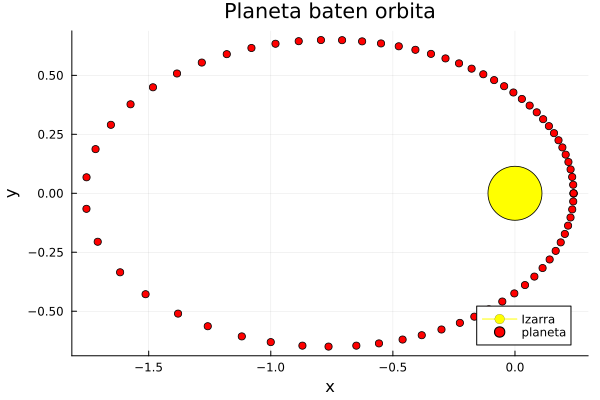
\includegraphics[width=0.7\linewidth]{sateliteae076}}
%    			  \centering \caption{\centering \tiny Gorputzen arteko gerturatzeak}
    		\end{minipage}
    	\end{figure}
    	
    	
    	  
    \end{itemize}
    
    
\note[item]
{

\begin{itemize}
\item Bigarren artikulu talde honetan, denbora-birnormalizazio teknika lantzen duten bi artikulu argitaratu ditugu.

\medskip
\item  N-gorputzetako problemetan gorputzen arteko gerturatzeak gerta ohi dira (adibidez planeta batek izar baten inguruko orbita eliptikoan) eta 
kasu horietan, zenbakizko integraziorako luzeera finkoko urratsa erabiltzea ez da eraginkorra.

\medskip
\item Arazo hau gainditzeko teknika bat, denbora-birnormlizazio da. Artikulu hauetan,  denbora-birnormalizaziorako funtzio berriak proposatzen dira eta integrazioan zehar  urrats luzera ondo egokitzea lortzen dugu

%Teknika hauei esker, N-gorputzetako grabitazio problemen urrats luzera finkoko simulazioen  eraginkortasuna hobetzen dugu. 
\end{itemize}






}

\end{frame}


%%%%%%%%%%%%%%%%%%%%%%%%%%%%%%%%%%%%%%%%%%%%%%%%%%%%%%%%%%%%%%%%%%%%%%%%%%%%%%%

\begin{frame}{Ikerketaren merezimenduak} 

\medskip

\textbf{Kongresutan parte hartzea}

\small
%Presentación de posters en los siguiente congresos internacionales:
\medskip
\begin{itemize}
%\item \textbf{EuroSoTL} - Junio 2019

%European Scholarship of Teaching and Learning Conference 

%Poster: Computational Notebooks: a powerful way to learn

%\medskip
\item \textbf{ICIAM} - Uztaila 2019

International Congress on Industrial and Applied Mathematics 

Posterra: FCIRK symplectic integrators  with application to high precision Solar System Simulations

%\medskip
%\item \textbf{IMCS-55} - Iraila 2019

%5th International Conference of Mathematical
%Society of Moldova

%Komunikazioa: An algorithm based on continuation techniques for minimization problems with non-linear equality constraints

\medskip
\item \textbf{JuliaCon2020} - Uztaila 2020

International Congress : Julia Programming Language 

Posterra: Implicit RK solver for high precision numerical integrations

\medskip
\item \textbf{JuliaCon2022} - Uztaila 2022 % \qquad \textcolor{red}{Laster !!!}

International Congress : Julia Programming Language 

Lighting talk:  SIMD-vectorized implementation of high
order IRK integrators

\end{itemize}


\note[item]{

\begin{itemize}
\item Lan hauek, gure ikerketa arloko errefentziazko kongresutan aurkeztu ditugu % direla azpimarratuz


\medskip
\item Batetik ICIAM kongresuan parte-hartzea, lau-urtean behin ospatzen den matematika aplikatuko nazioarteko kongresua

\medskip
\item Eta Julia lengoaiaren kongresuan parte-hartzea 


\end{itemize}



}

\end{frame}




%%%%%%%%%%%%%%%%%%%%%%%%%%%%%%%%%%%%%%%%%%%%%%%%%%%%%%%%%%%%%%%%%%%%%%%%%%%%%%%

\begin{frame}{Ikerketaren merezimenduak} 
	
	
	\medskip
	\medskip
	\textbf{Softwarea}: \textcolor{blue}{IRKGL16 inplementazioa}
	\small
	
	\medskip
	\begin{itemize}
		\item  SciML: Open Source Software for Scientific Machine Learning
		%
		%
		\begin{itemize}
			\item Julian garatutako errendimendu altuko softwarea
			\item  \textcolor{black}{Egungo EDAen zenbakizko integraziorako ekosistema hoberena? }
		\end{itemize}
		%
		\begin{figure}
			\begin{minipage}{1.\textwidth}
				\colorbox{white}  {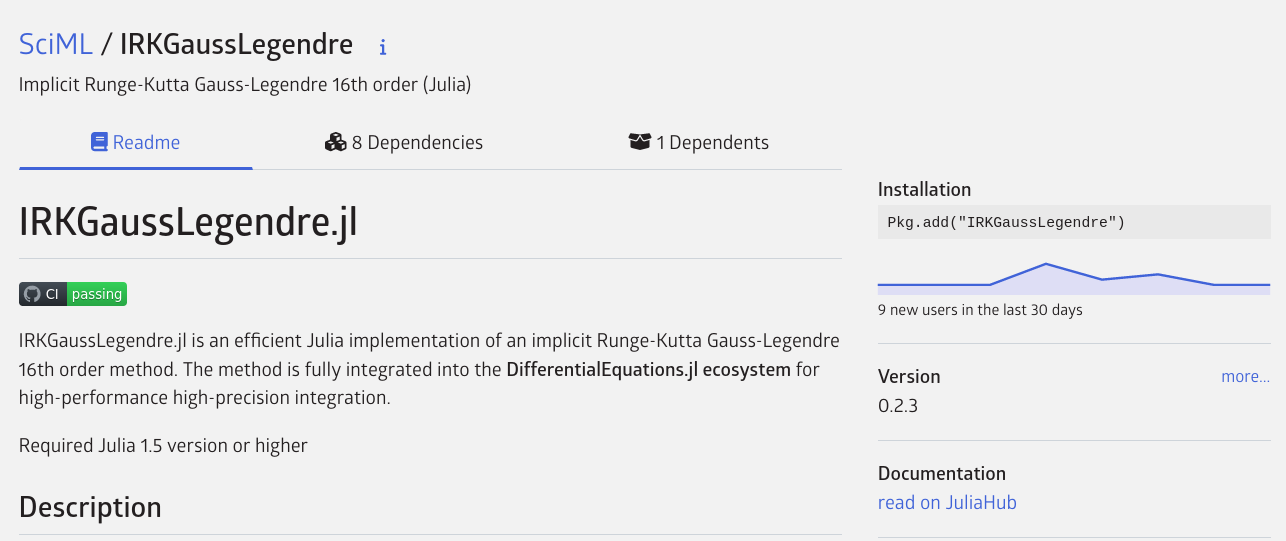
\includegraphics[width=0.8\linewidth]{SCIMLIRKGaussLegendre2023}}
			\end{minipage}
			%\end{figure}
			%
			%\begin{figure}
			%\begin{minipage}{.6\textwidth}
			%\colorbox{white}  {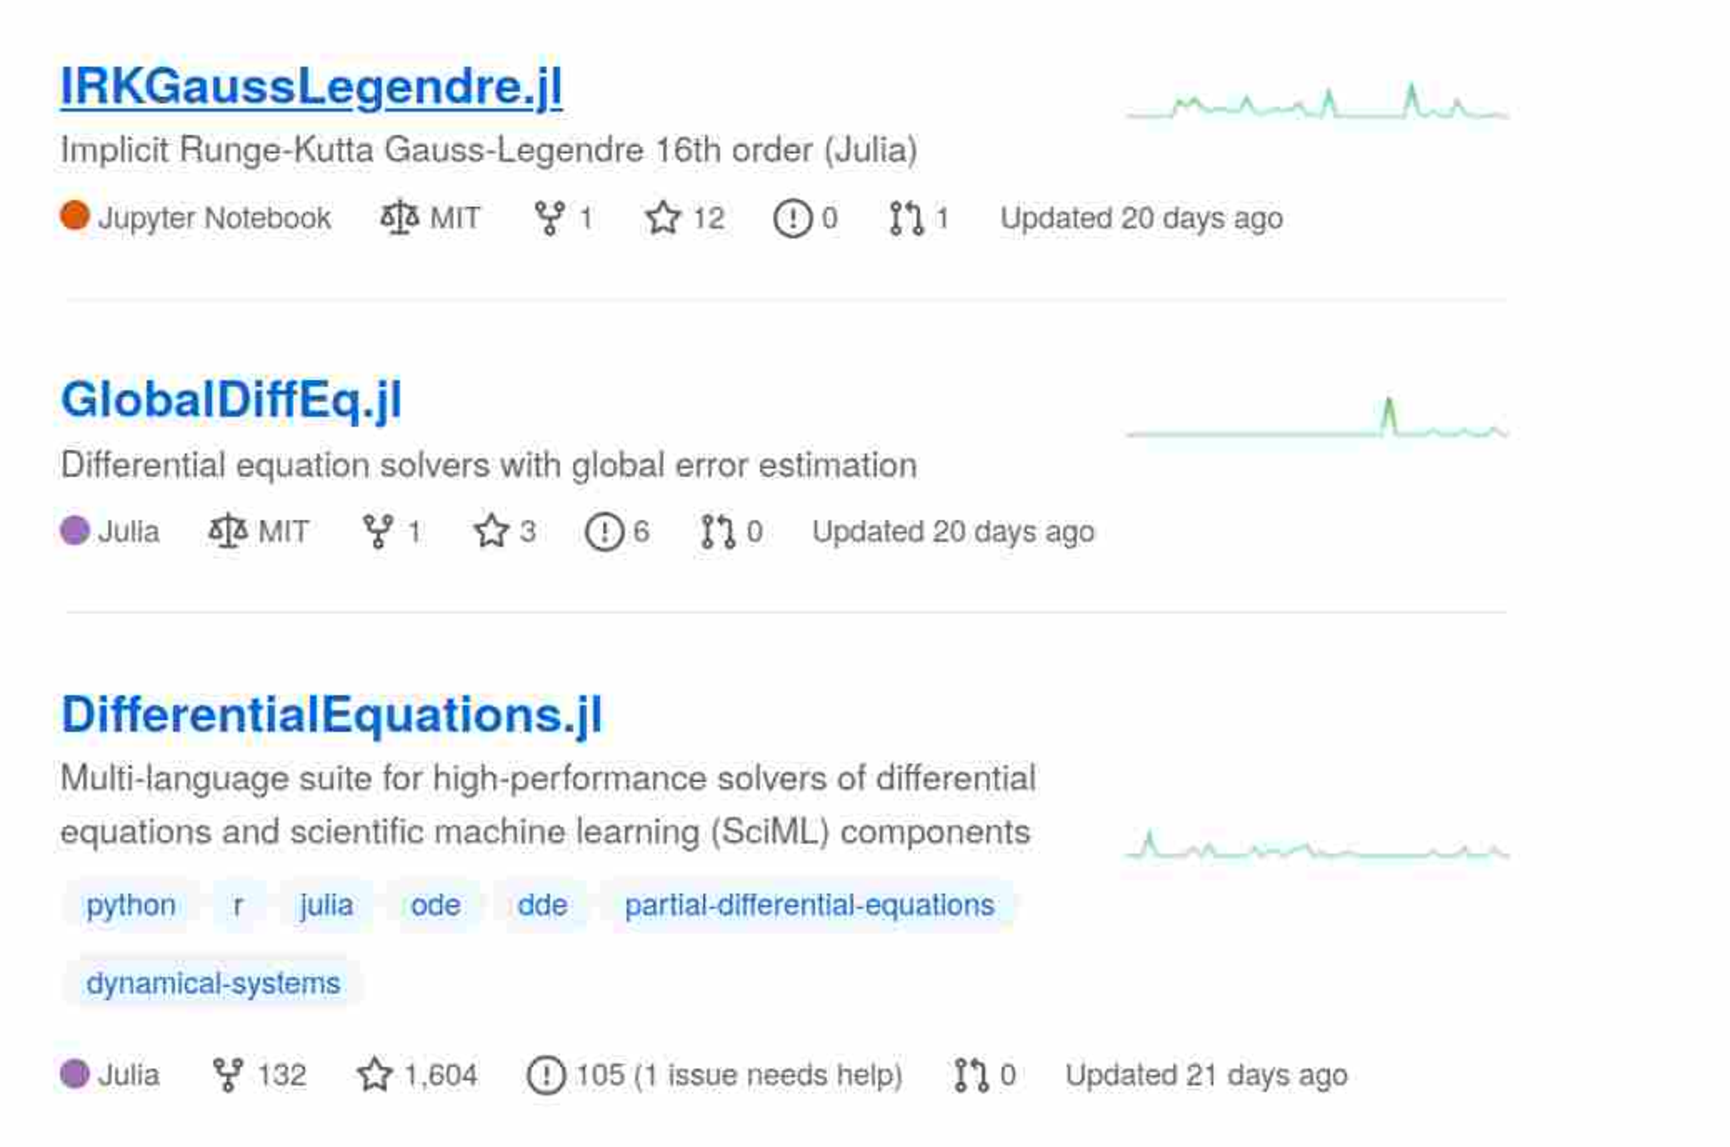
\includegraphics[width=1.\linewidth]{SciML-IRKG16}}
			%\end{minipage}
		\end{figure}
		%\end{itemize}
		
%		\medskip
		

		
%		\textcolor{black}{Matlab ODE, Mathematica ODE, SciPy (Python), C, Fortran, deSolve (R) \dots}
		
	\end{itemize}
	
	\note[item]{
		
		\begin{itemize}
			\item 2020. urteko Julia kongresuan aurkeztutako IRKGL16 metodoaren inplementazioa, SciML (open Source Software for Scientific Machine Learning) erakundeak bere bilguean gehitzeko aukera eskaini zigun
			
			\medskip
			\item Erakunde honek, bere bilgunean  Julian garatutako errendimendu altuko softwarea eskaintzen du.   
			
			\medskip
			\item Egun, Solftware-bilgune hau, EDAen zenbakizko integraziorako ekosistema hoberena dela esaten ausartuko nintzateke.
%			
%			berritzailea eskaintzen da eta beste sistema ezagunak (Matlab, Mathematica, Python, C, Fortran, ...) baino hobe dela esaten ausartuko nintzateke 
		\end{itemize}
		
		
		
	}
	
\end{frame}

%%%%%%%%%%%%%%%%%%%%%%%%%%%%%%%%%%%%%%%%%%%%%%%%%%%%%%%%%%%%%%%%%%%%%%%%%%%%%%%

\begin{frame}{Irakaskuntzaren eta ikerketaren  merezimenduak} 
	
\medskip

%\large
%\hspace*{3.cm} \textcolor{blue}{Laburpena}

%\normalsize
%\textbf{Irakaskuntzaren eta ikerketaren arloko merezimenduak}

%\bigskip

\Laburpena{Irakaskuntzaren eta ikerketaren  merezimenduak}
{

\medskip

\begin{itemize}
	
	\item[1)] 2017-2023: Irakasle \textbf{prestakuntza fase aberatsa}
	
%	 garapen profesionala hobetzeko gomendioak jarraitzea
	
	\medskip
	
	\item[2)] Ikerketa, KZAA sailaren arloarekin \textbf{ondo lerrokatuta}
	
	\medskip
	
	\item[3)]  Ikerketa zentratuta:
	\begin{itemize}
		\item IRKGL metodo inplizitu eta sinplektikoak
		\item N-gorputzetako problema
	\end{itemize}
	
	\medskip
	
	\item[4)] Gure ikerketaren \textbf{difusio ona} zaindu dugu% zabalarentzat eskuragarri
	
\end{itemize}

\medskip

}


\note[item]{

    • 
Beraz, “Irakaskuntzaren eta ikerketaren arloko merezimenduak” atalaren laburpen moduan esan:


\medskip

\begin{itemize}
\item Irakasle \textbf{formakuntza aldia} izan da niretzat

\medskip
\item Ikerketa  Sailaren irakaskuntzarekin ondo lerrokatuta

\medskip
\item Ikerketa zentratuta:
\begin{itemize}
	\item IRKGL método inplizituak eta sinplektikoak
	\item Problema nagusia, eguzki sistemaren simulazioa
\end{itemize}

\medskip
\item Artikuluak aldizkari onetan argitaratzea eta garatutako inplementazioak software errepositoriotan eskuragarri jartzea zaindu dugu
\end{itemize}


}


\end{frame}



%%%%%%%%%%%%%%%%%%%%%%%%%%%%%%%%%%%%%%%%%%%%%%%%%%%%%%%%%%%%%%%%%%%%%%%%%%%%%%%

\section[Ikerketa proiektua]{Ikerketa proiektua}

\begin{frame}{Ikerketa proiektua} 	
	
	\medskip
	  \tableofcontents[currentsection,currentsubsection]
	  
	
	\begin{figure}
		\begin{minipage}{.8\textwidth}
			\colorbox{white}  {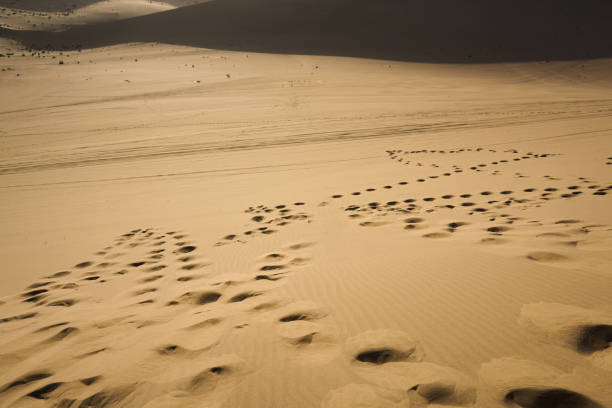
\includegraphics[width=0.8\linewidth]{Desertua}}
		\end{minipage}
	\end{figure}


\note{

\begin{itemize}
\item Behin irakaskuntzaren eta ikerketaren arloko merezimenduekin amaituta,
	ikerketa proiektuarekin hasiko naiz eta deskribapena bi zatitan banatu dut:

%
\begin{itemize}
	%\item Lehenik, ikerketaren lerro nagusiak  eta orain arte egindako lana  azalduko dut
	
	\medskip
	\item Lehenik, etorkizunerako hainbat proiektu  aipatuko ditut
	
	
	\medskip
	\item Eta bigarrenik ikerketaren balorazio txiki bat egingo dut
	
%	\begin{itemize}
		
		
%		\medskip
%		\item Bigarrenik,  Europako eta EEBBko plan teknologikoak aipatuz, gure ikerketaren errelebantzia defendatu nahiko nuke
		
		
%		\medskip
%		\item Hirugarrenik, software librearen eta bereziki Julia lengoaiaren aldeko apostua argudiatuko dut  
		
%		\medskip
%		\item Laugarrenik, gradu eta masterreko irakaskuntzari ekarpenak egiteko moduko ikerketa egiten dugula
		
%	\end{itemize}

\end{itemize}

\end{itemize}

}

\end{frame}

%%%%%%%%%%%%%%%%%%%%%%%%%%%%%%%%%%%%%%%%%%%%%%%%%%%%%%%%%%%%%%%%%%%%%%%%%%%%%%%

%\section[Ikerketa proiektua]{Ikerketa proiektua}

%\begin{frame}{Ikerketa proiektua} 	

%\medskip

%\begin{itemize}
%\item[1)] Ikerketa lerroak
%\item Difusión (repositorios software)

%\item[1)] Etorkizunerako proiektuak

%\item[2)] Ikerketaren alde garrantzitsuak
%
%Alineación con los planes de ciencia y tecnología
%\item[3)] Software librea eta Julia
%
%\item[4)] Gradu eta Masterreko irakaskuntzari ekarpenak

%\end{itemize}

%\bigskip

%\begin{figure}
%
%\begin{minipage}{.3\textwidth}
%\colorbox{white}  {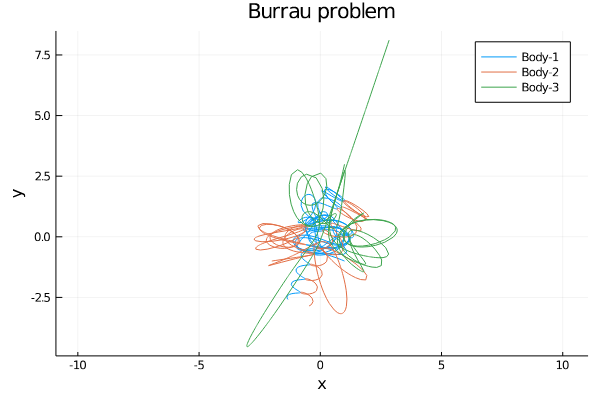
\includegraphics[width=0.8\linewidth]{BurrauOrbits}}
%\end{minipage}
%
%\begin{minipage}{.3\textwidth}
%\colorbox{white}  {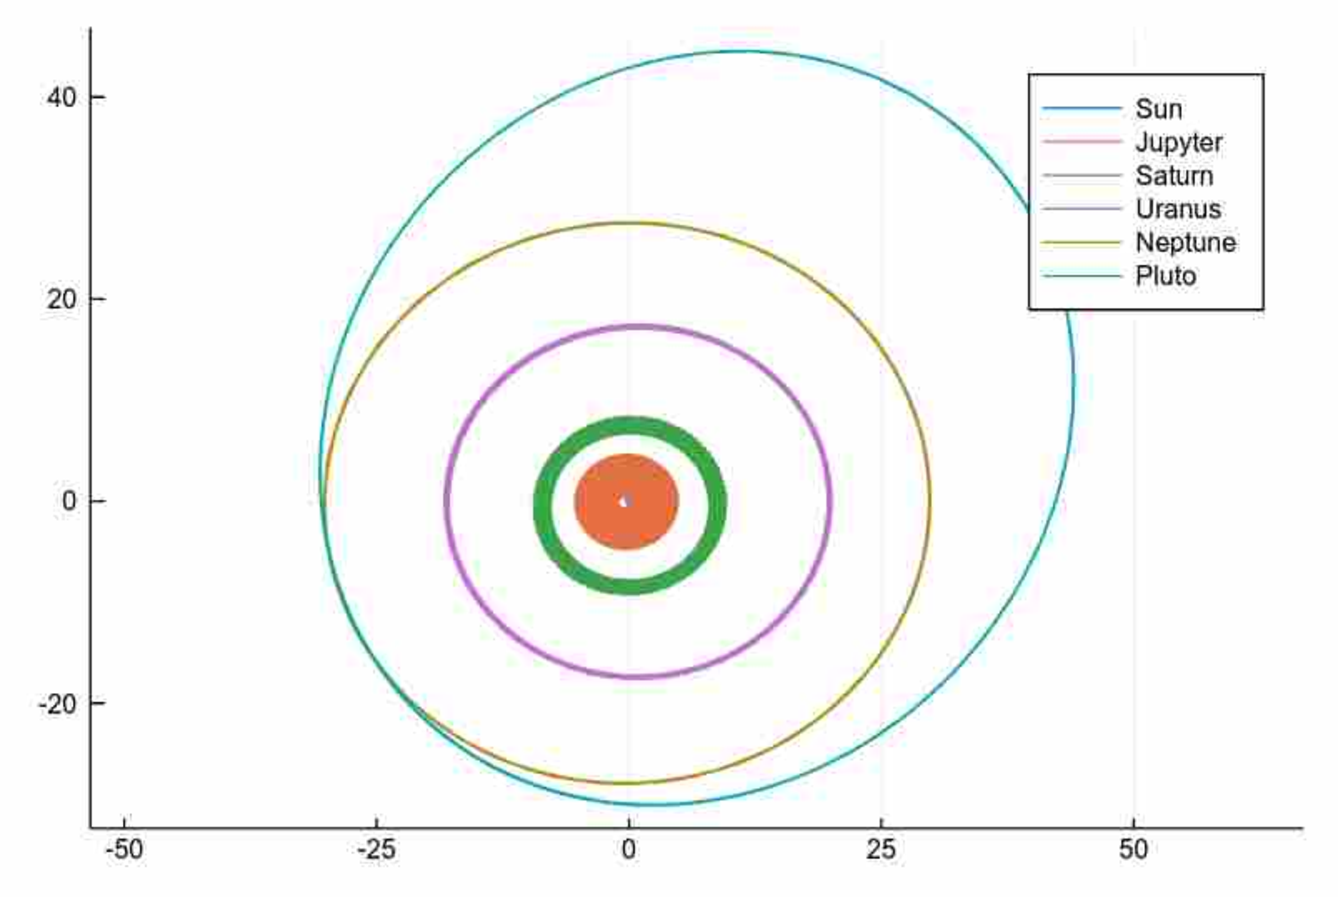
\includegraphics[width=0.8\linewidth]{EguzkiSistema}}
%\end{minipage}
%
%\begin{minipage}{.3\textwidth}
%\colorbox{white}  {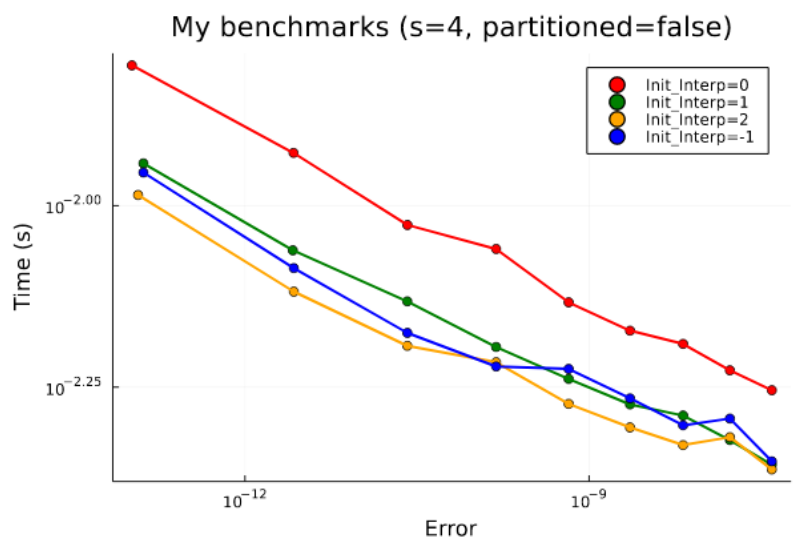
\includegraphics[width=0.8\linewidth]{benchmark_adba}}
%\end{minipage}
%
%\end{figure}
%
%\begin{figure}
%
%\quad
%\begin{minipage}{.3\textwidth}
%	\colorbox{white}  {
\includegraphics[width=0.8\linewidth]{SoftwareLibre}}
%\end{minipage}
%
%\begin{minipage}{.3\textwidth}
%\colorbox{white}  {
\includegraphics[width=0.6\linewidth]{julia-logo-color}}
%\end{minipage}
%
%\begin{minipage}{.3\textwidth}
%\colorbox{white}  {
\includegraphics[width=0.8\linewidth]{Horizon27}}
%\end{minipage}
%
%
%\end{figure}


%\note[item]{

%Ikerketa proiektuaren deskribapena bi zatitan banatu dut:
%
%\medskip
%\begin{itemize}
%\item Lehenik, ikerketaren lerro nagusiak  eta orain arte egindako lana  azalduko dut

%\medskip
%\item Lehenik, etorkizunerako proiektuak ideia batzuk laburtuko ditut


%\medskip
%\item Eta bigarrenik ikerketaren alde garrantzitsuak nabarmenduko ditut

%\begin{itemize}


%\medskip
%\item Bigarrenik,  Europako eta EEBBko plan teknologikoak aipatuz, gure ikerketaren errelebantzia defendatu nahiko nuke

%ikerketa lerro horiek  Horizon Europa estrategian nola jasotzen diren azpimarratuko dut  


%\medskip
%\item Hirugarrenik, software librearen eta bereziki Julia lengoaiaren aldeko apostua argudiatuko dut  

%\medskip
%\item Laugarrenik, gradu eta masterreko irakaskuntzari ekarpenak egiteko moduko ikerketa egiten dugula

%\end{itemize}

%\end{itemize}


%}


%\end{frame}
%%%%%%%%%%%%%%%%%%%%%%%%%%%%%%%%%%%%%%%%%%%%%%%%%%%%%%%%%%%%%%%%%%%%%%%%%%%%%%%


%\begin{frame}{1) Ikerketa lerroak} 	



%
%\textbf{Arloa?}

%\medskip

%\color{blue}

%\textbf{Konputazio zientzia:} 

%\hspace*{1.8cm} \color{black} Modelizazioa + Zenbakizko simulazioa+ Programazioa


%
%\begin{itemize}
	
%\medskip
	%

%\small
%\color{black}


%\medskip

%\item[1)] \textbf{Problemak?} 
%
%\medskip
%
%\textcolor{blue}{\textbf{-$N$ gorputzen} problema grabitazionalaren simulazioak }
%
%\begin{align*}
%\text{N-gorputzetako problemak} \quad
%
%\begin{cases}
%\text{\textcolor{blue}{\textbf{-Eguzki sistema} }} \\
%\text{\textcolor{blue}{\textbf{-Sateliteen} propagazio orbitalak}}
%\end{cases}
%\end{align*}


%\medskip

%\textcolor{blue}{\textbf{- Scientific Machine Learning:}
%		Gradientearen kalkulua  }
%(Espazioko Mekanika eta Astrodinamika)}
%




%\medskip

%\item[2)] \textbf{Zenbakizko Metodoak?}
%
%\begin{align*}
%\begin{cases}
%\textcolor{blue}{\textbf{- RK metodo inplizituak }} \\ %, \\ sinplektikoak eta ordena altukoak}
%
%\textcolor{blue}{\textbf{- Taylor-Fourier metodoak}}
%
%\end{cases}
%\ \Rightarrow \ \text{Propietate onak}
%\ \Rightarrow \ \text{Bide berriak}
%\end{align*}

%

%\medskip

%\item[3)] \textbf{Helburua?}

%\medskip

%\textcolor{blue}{\textbf{Inplementazio sendoak eta eraginkorrak}}


%\medskip

%\item[3)] \textbf{Lengoiaia?}

%\medskip
%Julia

%\end{itemize}


%\note[item]{


%\begin{itemize}
%\item Gure ikerketa, konputazio zientzia arloan kokatzen da eta zehazki, EDAk modelizatutako problemen zenbakizko integraziorako metodo aurreratuen analisia eta inplementazioa.

%\medskip
%\item %N gorputzen problema grabitazionalaren: batetik, 
%Gure eredu nagusiena N-gorputzetako problema da. Haisera batean formulazio oso simple duen problema da baina oso konportamendu aberatsak dituena.
%Horien artean, Eguzki-sistemaren simulaziorako eta satelite artifizialen propagazio orbitalerako algoritmoak hobetu nahi ditugu

%\medskip
%\item Dena den eskuartean ere badugu Machine Learning arloko zeregin bat, zehazki,  Gradientea zehatzaren kalkulurako teknika berri bat   

%\medskip
%\item Bai eguzki-sistemaren simulazioetarako, bai sateliteen propagazio orbitalen kalkulutarako, ohikoak ez diren metodoak aplikatzea defenditzen dugu. Metodo hauek propietate konputazional eta matematiko onak dituztenez, inplementzeko bide berriak eskaintzen dizkigute

%\medskip
% Azken hamarkadetan zenbakizko integrazio metodoetan eman diren aurrerapenak aplikazea da, inplementazio sendoak eta eraginkorrak lortzeko (kalitatezko inplementazioak eraikitzea) 

%\medskip
%\item Julia: konputazio zientifikorako lengoaia

%\end{itemize}




%}

%\end{frame}





%%%%%%%%%%%%%%%%%%%%%%%%%%%%%%%%%%%%%%%%%%%%%%%%%%%%%%%%%%%%%%%%%%%%%%%%%%%%%%%


%\begin{frame}{1) Ikerketa lerroak} 	
	
		
%\medskip
%\small

%\Adibidea{ FCIRK,  eguzki sistemaren doitasun handiko zenbakizko integraziorako metodoa}
%{

%\begin{itemize}
	
%\item FCIRK metodoa
%
%\begin{figure}
%	\begin{minipage}{.9\textwidth}
%		\colorbox{white}  {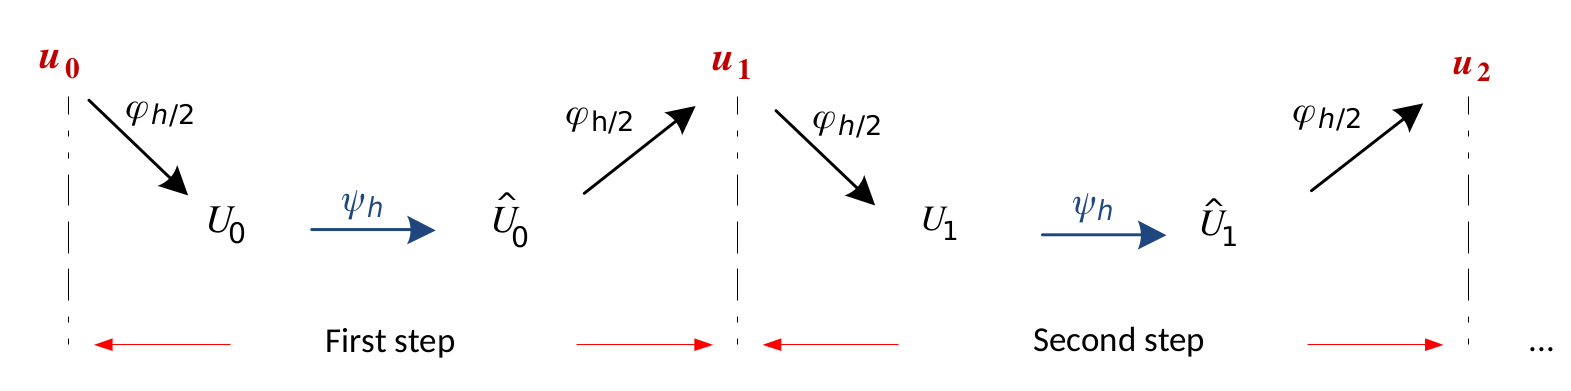
\includegraphics[width=0.9\linewidth]{FCIRK_diagrama}}
		%  \centering \caption{\centering \tiny wikipedia}
%	\end{minipage}
%\end{figure}

%\medskip
%\item Zenbakizko integrazioa

%\begin{figure}
%	\begin{minipage}{.4\textwidth}
%		\colorbox{white}  {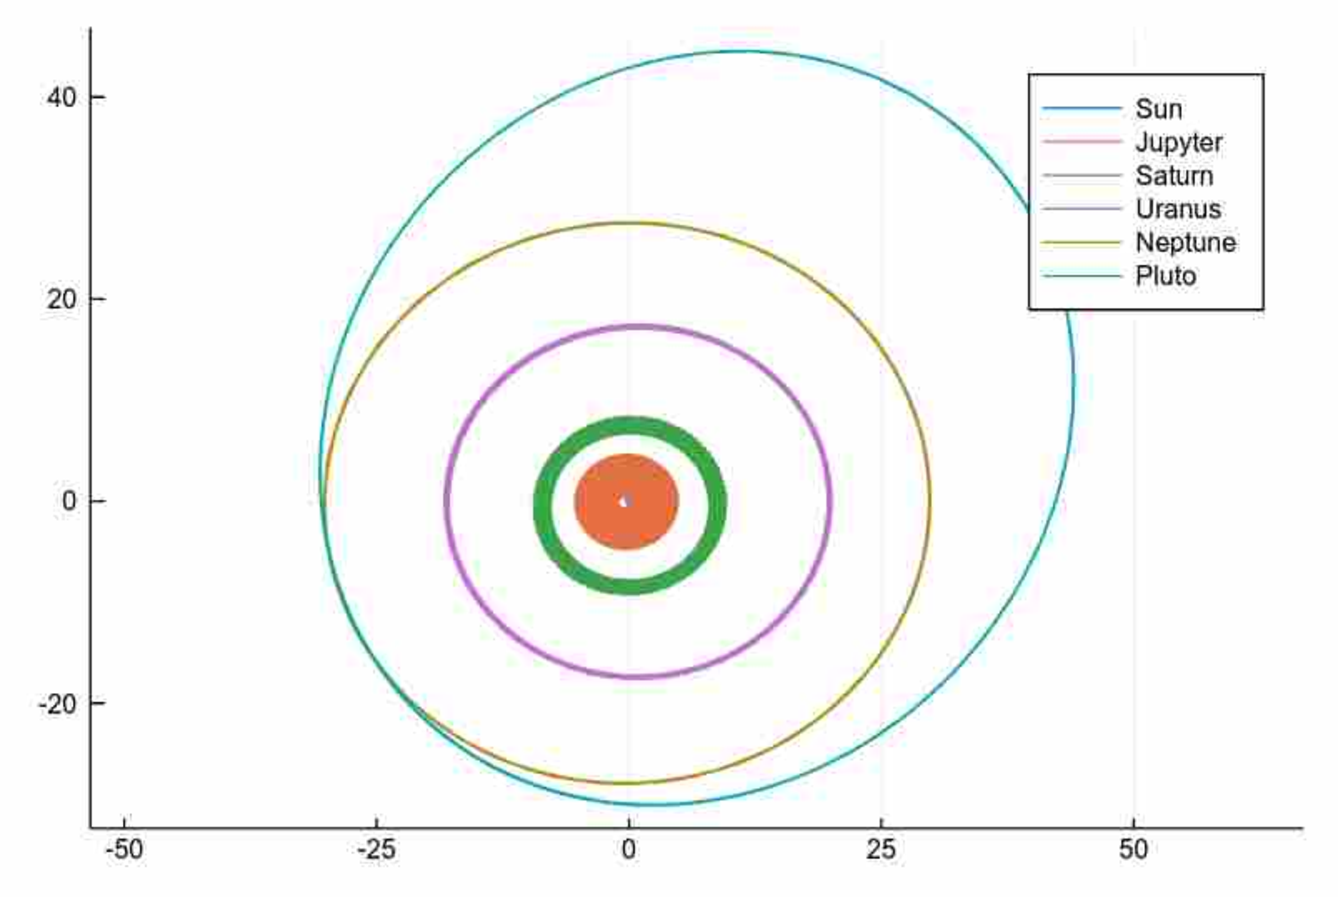
\includegraphics[width=0.9\linewidth]{EguzkiSistema}}
		%  \centering \caption{\centering \tiny wikipedia}
%	\end{minipage}
%
%   	\begin{minipage}{.4\textwidth}
%   	\colorbox{white}  {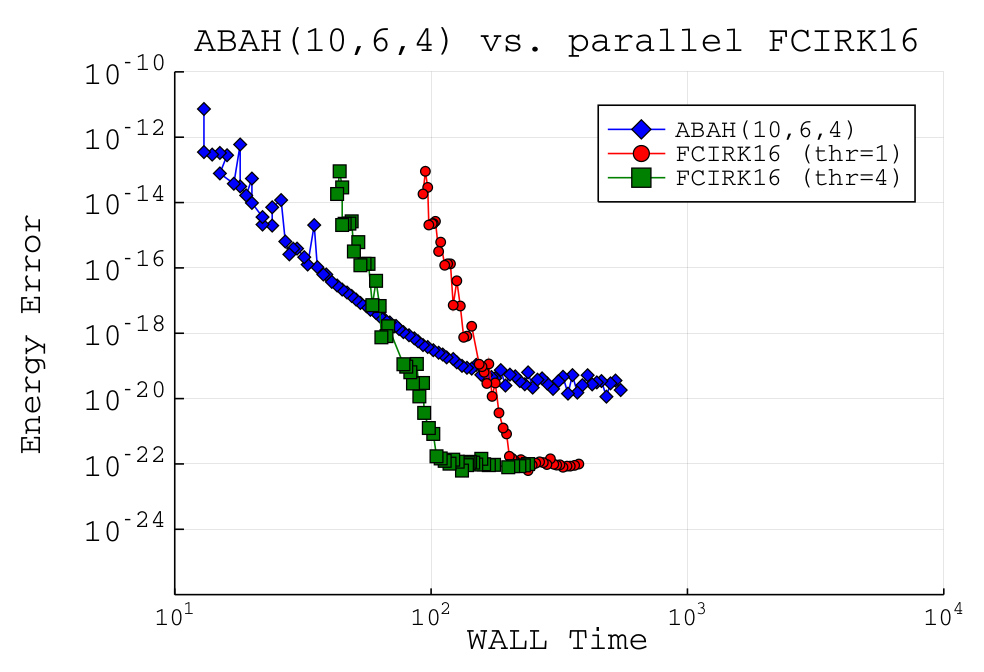
\includegraphics[width=0.9\linewidth]{FCIRK_Energia}}
    	%  \centering \caption{\centering \tiny wikipedia}
%    \end{minipage}
%\end{figure}

	
%\end{itemize}


%\note{

%\begin{itemize}
%	\item Azalpenak ...
	 
%\end{itemize}



%}

%}

%\end{frame}	




%%%%%%%%%%%%%%%%%%%%%%%%%%%%%%%%%%%%%%%%%%%%%%%%%%%%%%%%%%%%%%%%%%%%%%%%%%%%%%%


%\begin{frame}{1) Ikerketa lerroak} 	
	
	
	%\medskip
%	\small
	
%	\Adibidea{ Denbora birnormalizaziorako funtzioak N-gorputzetako problemaren integraziorako}
%	{
		
%		\begin{itemize}
			
%			\item Gorputzen gerturatzeak
			%
            %
			
%			\begin{figure}
%				\begin{minipage}{.9\textwidth}
%					\colorbox{white}  {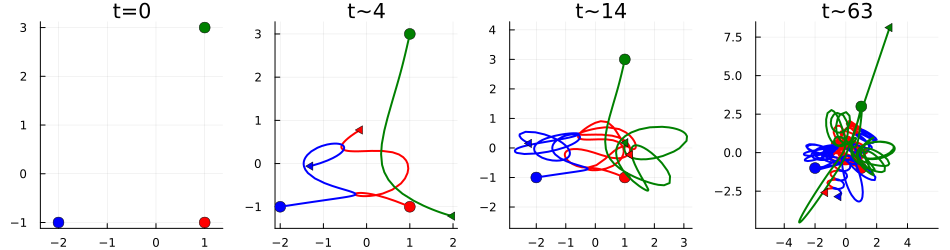
\includegraphics[width=0.9\linewidth]{PythagoreanP}}
					%  \centering \caption{\centering \tiny wikipedia}
%				\end{minipage}
				%
%			\end{figure}
		

%		\item Denbora birnormalizaziorako funtzioa: $\color{red} s(q,v)$
		%
%		\begin{align*}
%		& \frac{d\hat{q}_i}{d\tau}= \color{red} s(\hat{q},\hat{v}) \ \color{black} \hat{v}_i\\
%		& \frac{d\hat{v}_i}{d\tau}=\color{red} s(\hat{q},\hat{v}) \color{black} \ \sum_{j \ne i}{\frac{Gm_j}{\|\hat{q}_i-\hat{q}_j\|^3}} (\hat{q}_j-\hat{q}_i)
%		\end{align*}
			
			
%		\end{itemize}
		
		
%		\note{
			
%			\begin{itemize}
%				\item Azalpenak
				
%			\end{itemize}
			
			
			
%		}
		
%	}
	
%\end{frame}	




%%%%%%%%%%%%%%%%%%%%%%%%%%%%%%%%%%%%%%%%%%%%%%%%%%%%%%%%%%%%%%%%%%%%%%%%%%%%%%%


\begin{frame}{1) Etorkizunerako proiektuak} 	
	
	
\bigskip
\small

\begin{figure}
	\centering
	\begin{minipage}{1.\textwidth}
		\colorbox{white}  {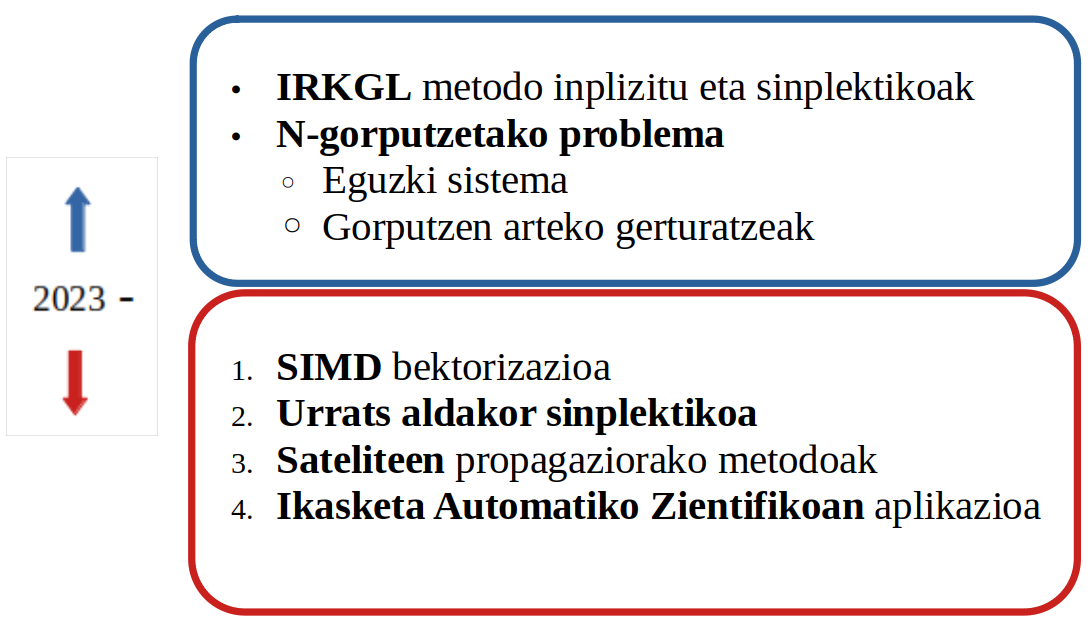
\includegraphics[width=1.\linewidth]{Etorkizunerako_proiektuak}}
		%		\centering \caption{\centering \tiny Learning the parts of objects by non-negative matrix factorization, (Nature, Lee and Seung, 1999)}
	\end{minipage}
\end{figure}


\note{

\begin{itemize}
	\item Orain arteko lanean, bi izan dira zutabe nagusiak:
	
	\medskip
	\begin{itemize}
		\item Batetik, IRKGL16 metodo inplizitu eta sinplektikoa
		\item Bestetik, N-gorputzerako problema. Horien artean nagusiki, 
		%
		\medskip
		\begin{itemize}
			\item Eguzki sistemaren simulazioan
			\item Gorputzen arteko gerturatzeak sortzen dituzten zailtasunen konponbideetan
		\end{itemize}
	    zentratu gara
		
	\end{itemize}
	
	\medskip
	
	\item Etorkizunean, batetik gai hauetan sakontzea eta bestetik aplikazio berriak aztertzea da gure asmoa. Jarraian, etorkizunerako lau proiektu horiek azalduko ditut.
	
%	\medskip
	
%	\begin{itemize}
%		\item SIMD bektorizazioa
		%
%		\item Sateliteen propagaziorako metodoak
		%
%		\item Urrats aldakor sinplektikoa, N-gorputzerako problemarentzat
		%
%		\item Ikasketa Zientifiko Arloko optimizazio problemen gradienteen kalkulurako, metodo inplizitu sinplektikoen abantaila erakutsi nahi dugu
		
%	\end{itemize}
	
\end{itemize}




}

\end{frame}


%%%%%%%%%%%%%%%%%%%%%%%%%%%%%%%%%%%%%%%%%%%%%%%%%%%%%%%%%%%%%%%%%%%%%%%%%%%%%%%


%\begin{frame}{1) Etorkizunerako proiektuak} 	
	
	
%	\bigskip
%	\small
	
	
	
%	\begin{table}[h!]     
%		\centering
%		{%
%		\begin{tabular}{ l l} 
% \large \color{ blue} RK inplizituak      &   \large \color{ blue} \large Sateliteak \\ \\
% SIMD bektorizazioa &  Propagazio metodo berriak \\ \\ 
%\\
 
%  \large \color{ blue} N-Gorputzetako problemak &  \large \color{ blue} Ikasketa Automatiko Zientifikoa \\ \\
% Urrats aldakorra (sinplektikoa) &  Gradienteen kalkulua
%		\end{tabular}}
%	\end{table}
	
		
	
		
		
%		\note{
			
%			\begin{itemize}
%				\item Runge-Kutta metodo inplizituen inplementazioaren arloan, egungo ordenagailuek eskaintzen duten SIMD-bektorizazioari etekina atereaz, metodo inplizutek, metodo explizituak baino eraginkorragoak izan daitezkeela erakutsi nahi dugu.
				
%				\medskip
%				\item Egun espazioan dagoen satelite kopurua oso handia denez, hauen arteko kolisioak ebitatzeko, sateliteen orbiteen kalkulurako doitasun altuko metodo eraginkorrak beharrezkoak dira.
				
%				\medskip
%				\item Urrats aldakorreko estrategia estandarrak ez dira egokiak zenbakizko metodo geometrikoetan aplikatzeko (hauek bere propietate onak galtzen baituzte). Denbora birnormalizazio tekniken lanari jarraipena emanez, N-gorputzetako probemarentzat urrats aldakor simplektikoa garatu nahi dugu
				
%				\medskip
%				\item Ikasketa Automatiko Zientifiko arloko optimizazio problemen gradienteen kalkulurako, metodo inplizitu sinplentikoen abantaila erakutsi nahi dugu
				
				
%			\end{itemize}
			
%		}
			
	

	
%\end{frame}	




%%%%%%%%%%%%%%%%%%%%%%%%%%%%%%%%%%%%%%%%%%%%%%%%%%%%%%%%%%%%%%%%%%%%%%%%%%%%%%%


\begin{frame}[fragile]{1) Etorkizunerako proiektuak} 	
	
	
\medskip
\small

\begin{itemize}
	
	\item[1)] \textcolor{blue}{ IRKGL16 inplementazio SIMD-bektorizatua}
	

		\begin{figure}
			\centering
			\begin{minipage}{0.5\textwidth}
				\colorbox{white}  {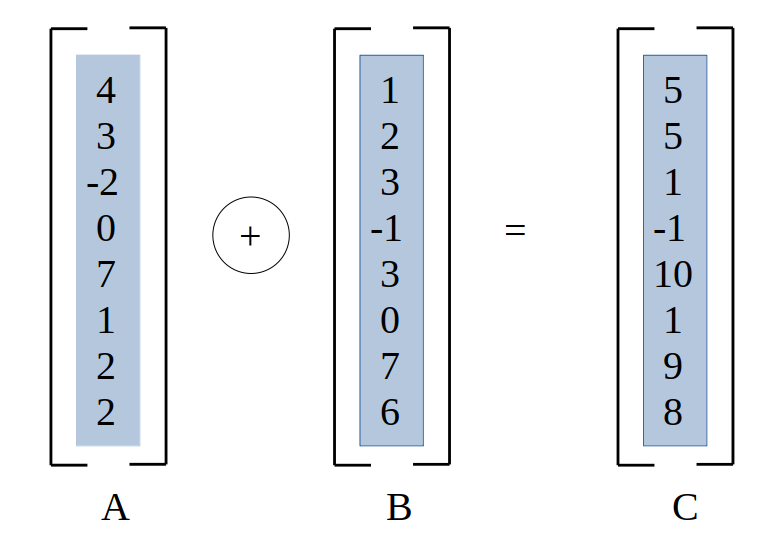
\includegraphics[width=0.5\linewidth]{SIMD}}
						\centering \caption{\centering \tiny SIMD-unitatea}
			\end{minipage}
		\end{figure}
		
	
	
	\item[2)] 	\textcolor{blue}{N-gorputzetako problemarentzat urrats aldakor sinpektikoa}
	
	\bigskip
	
	\begin{figure}
		\centering
		\begin{minipage}{.9\textwidth}
			\colorbox{white}  {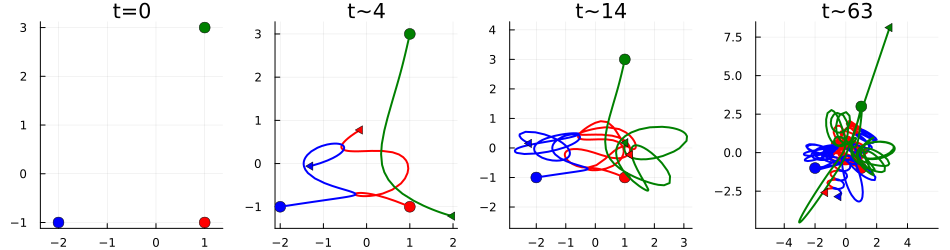
\includegraphics[width=0.9\linewidth]{PythagoreanP}}
			\centering \caption{\centering \tiny Problema Pitagorearra}
		\end{minipage}
		%
	\end{figure}
\end{itemize}


%\textcolor{blue}{1) IRKGL16 inplementazio SIMD-bektorizatua}


%\medskip

%\begin{columns}


%\column{0.5\textwidth}

%\centering SIMD-unitatea
%\begin{figure}
%	\begin{minipage}{0.9\textwidth}
%		\colorbox{white}  {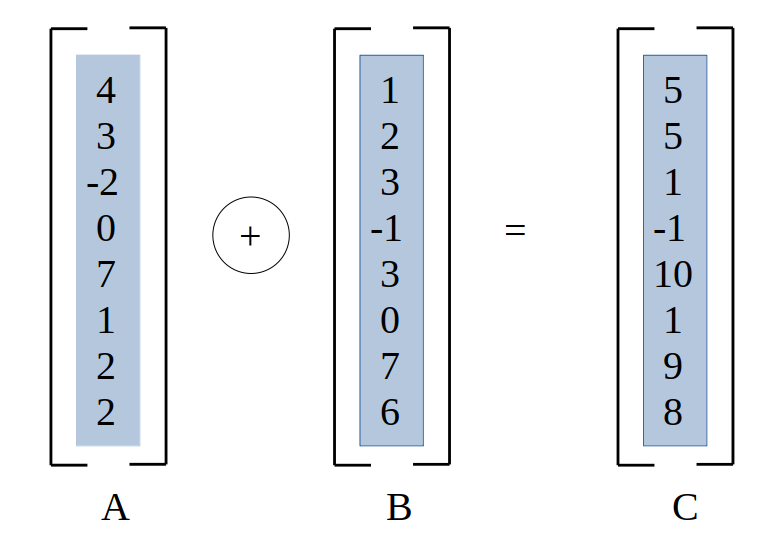
\includegraphics[width=0.9\linewidth]{SIMD}}
		%		\centering \caption{\centering \tiny Learning the parts of objects by non-negative matrix factorization, (Nature, Lee and Seung, 1999)}
%	\end{minipage}
%\end{figure}


%\column{0.5\textwidth}



%\hspace*{1.cm} IRKGL kode sekuentziala 

%\vspace*{1.cm}

%for $(k=1,2,3, \dots)$ do
%\begin{align*}
%&\quad L_{i}^{[k-1]}=hb_i f(t+c_i, Y_{i}^{[k-1]}), \quad i=1,\dots,8 \\
%&\quad Y_{i}^{[k]}=y+\sum_{j=1}^{8} \mu_{ij} L_{j}^{[k-1]}
%\end{align*}
%end


%\begin{code}
%for is in 1:s
%	f(F[is], U[is], p,  tj  + sdt*c[is])
%	for k in indices
%		U_[is][k] = U[is][k]
%		L[is][k] = sdt*(b[is]*F[is][k])
%	end
%end


%for is in 1:s
%	for k in indices
%	  dUik = muladd(mu[is,1], L[1][k], ej[k])
%	  for js in 2:s
%	    dUik = muladd(mu[is,js], L[js][k], dUik)
%	  end
%	  U[is][k] =  uj[k] + dUik
%	end
%end
%\end{code}


%\end{columns}




	
\note{
	
	\begin{itemize}
		
		
		\item  Egungo CPUek konputazioak azkartzeko, eragiketak bektorialki exekutatzeko gaitasuna dute eta teknologi honi  Single instruction multiple data (SIMD) esaten zaio. %Tipikoki SIMD unitate batek bi bektore jasotzen ditu,  bektore-osagaien guztien artean eragiketa bera burutzen du eta bektore bat itzultzen du emaitzarekin.    
		
		\medskip
		\item Proiektu honetan ideia da, IRKGL16 metodoak, eraginkortasuna hobetzeko SIMD-bektorizazioari etekina atera diezaiokeen aztertzea
%		 $8$ luzerako bektoreen gaineko konbinazio linealak kalkulatzen dituenez, SIMD-bektorizazioari etekin atera diezaioke eraginkortasuna hobetzeko.

		
		\medskip
	\item Bigarren ideiari helduz, esan, urrats aldakorreko estrategia estandarrak ez dira egokiak zenbakizko metodo sinplektikoetan aplikatzeko (hauek bere propietate onak galtzen baituzte). Denbora birnormalizazio tekniken lanari jarraipena emanez, N-gorputzetako probemarentzat urrats aldakor sinplektikoa garatu nahi dugu
		
		
%		\item Runge-Kutta metodo inplizituen inplementazioaren arloan, egungo ordenagailuek eskaintzen duten SIMD-bektorizazioari etekina atereaz, metodo inplizutek, metodo explizituak baino eraginkorragoak izan daitezkeela erakutsi nahi dugu.
		
		
		
	\end{itemize}
	
}





\end{frame}


%%%%%%%%%%%%%%%%%%%%%%%%%%%%%%%%%%%%%%%%%%%%%%%%%%%%%%%%%%%%%%%%%%%%%%%%%%%%%%%


\begin{frame}[fragile]{1) Etorkizunerako proiektuak} 	
	
	
	\medskip
	\small


\textcolor{red}{Aplikazioa berriak !!}	

\medskip

\begin{itemize}
	\item[3)]  	\textcolor{blue}{ Sateliteen propagaziorako metodoak}
	
\medskip


\begin{figure}
\begin{minipage}{.45\textwidth}
	\colorbox{white} 
	{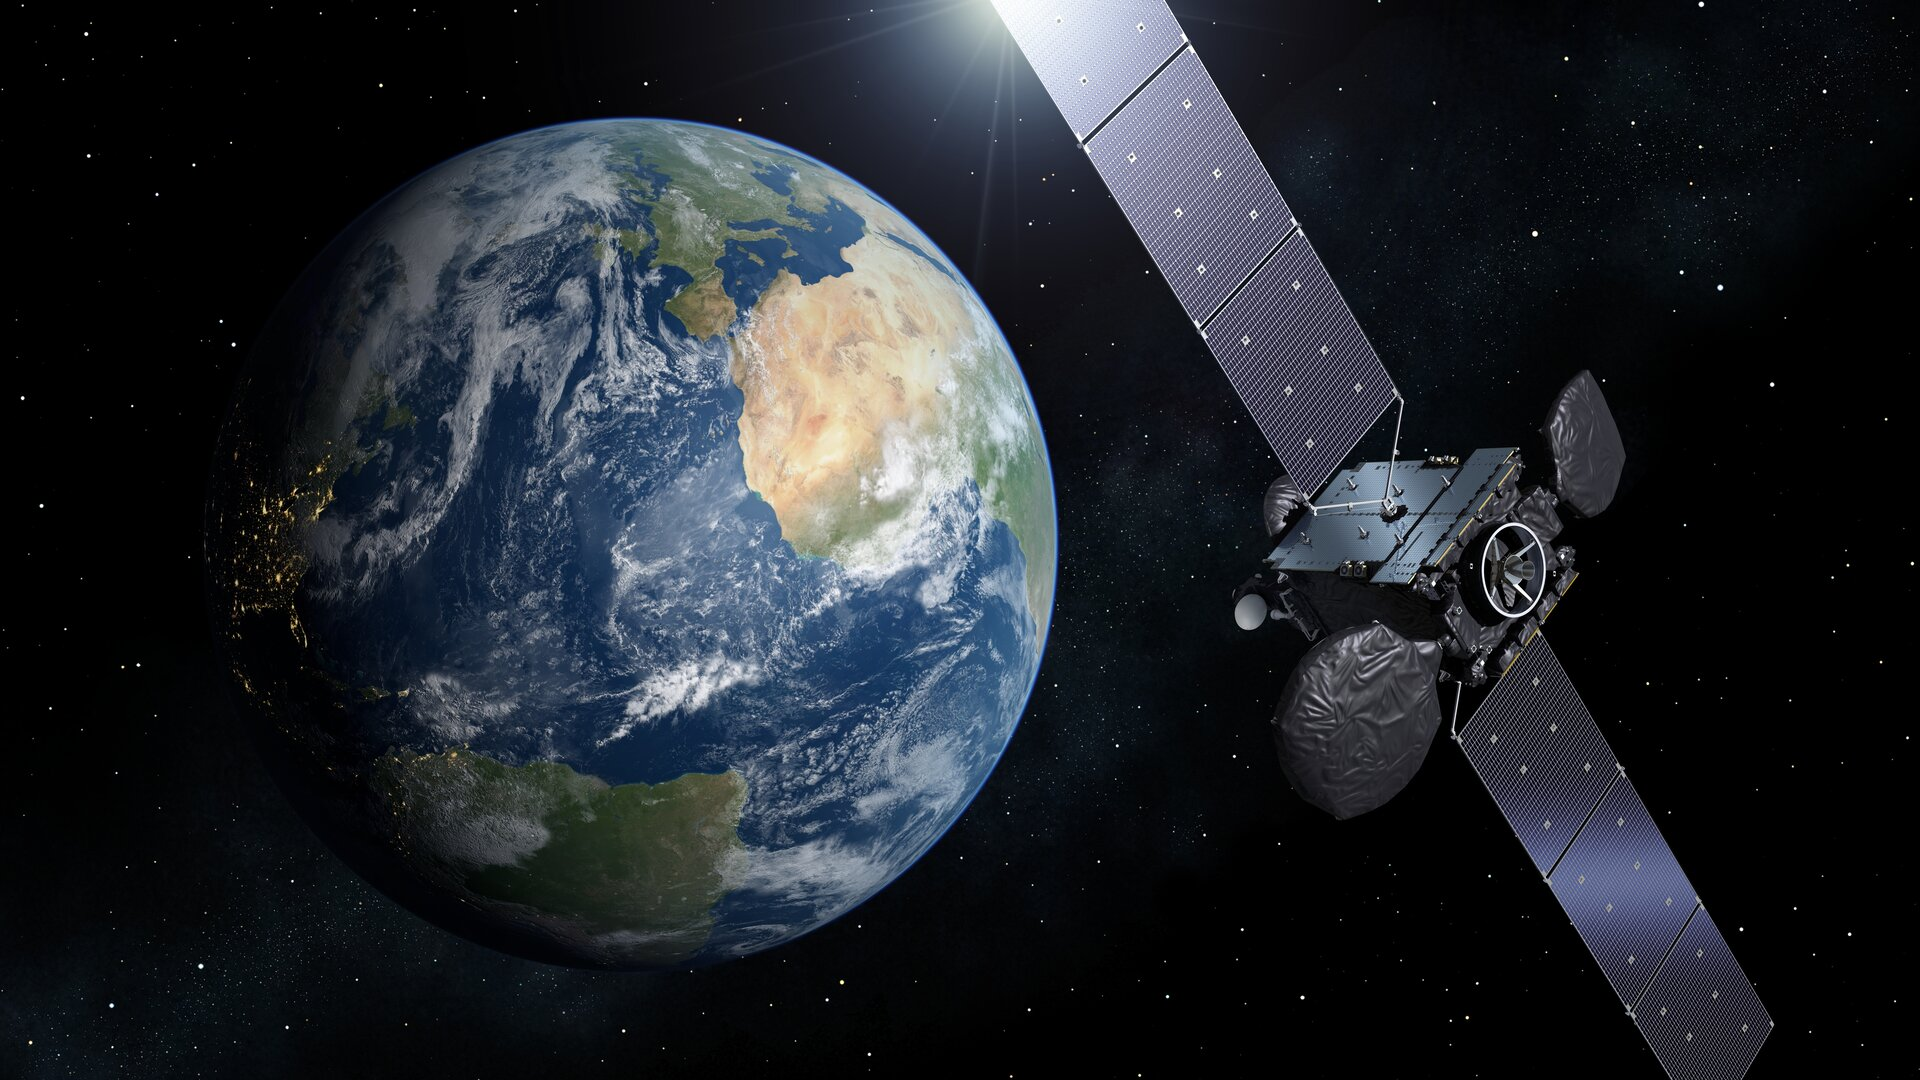
\includegraphics[width=0.8\linewidth]{SmallGEO_Hispasat_36W-1_pillars}}
\end{minipage}
%
\begin{minipage}{0.45\textwidth}
	\colorbox{white}  {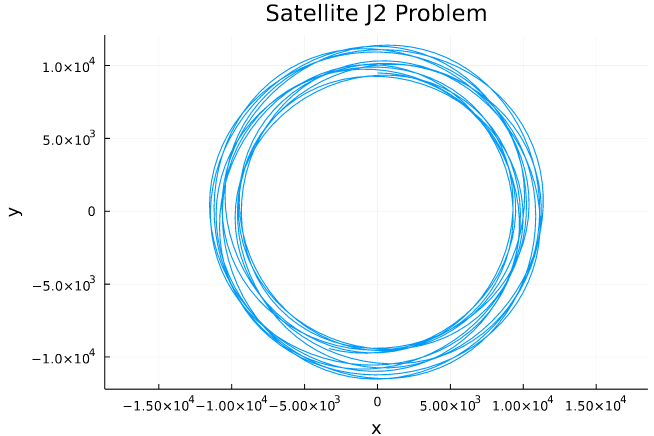
\includegraphics[width=0.8\linewidth]{J2 VOP Problem}}
\end{minipage}
\end{figure}

\medskip

\item[4)] 	\textcolor{blue}{Ikasketa Automatiko Zientifikoa arloan aplikazioa}


\begin{figure}
	\begin{minipage}{.45\textwidth}
		\colorbox{white} 
		{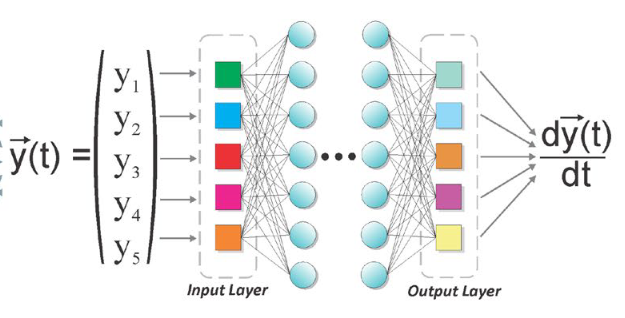
\includegraphics[width=0.8\linewidth]{Ikasketa_Automatiko_Zientifikoa}}
	\end{minipage}
	%
\end{figure}


\end{itemize}

\note{


Etorkizunerako beste bi proiektuak, aplikazio berriak ditugu:
	
\begin{itemize}
	
	\item 	Egun espazioan dagoen satelite kopurua oso handia denez, hauen arteko kolisioak ebitatzeko, sateliteen orbiteen kalkulurako doitasun altuko metodo eraginkorrak beharrezkoak dira.
	
	IRKGL metodoek, problema kontserbakorren epe luzeko eta doitasun altuko zenbakizko integrazioetarako propietate interesgarriak dituztenez, metodo hauek sateliteen orbiten kalkulurako egokiak izatea espero liteke.

	

	
	\medskip
	\item 	 Eta etorkizuneko proiektuekin amaitzeko, Ikasketa Automatiko Zientifiko arloan, optimizatu behar diren funtzioen  ebaluaziorako, ekuazio diferentzialen zenbakizko soluzioa kalkulatzea beharrezkoa da. Optimizazio algoritmoek helburu funtzioaren gradientea askotan kalkulatu behar dute eta IRKGL metodoak, hauek  modu eraginkorrean kalkulatzeko aplikatu daitezke
	
	
\end{itemize}




}




\end{frame}



%%%%%%%%%%%%%%%%%%%%%%%%%%%%%%%%%%%%%%%%%%%%%%%%%%%%%%%%%%%%%%%%%%%%%%%%%%%%%%%


\begin{frame}{2) Ikerketa proiektuaren balorazioa}
	
	
\bigskip

	
	
\begin{itemize}
	\item[1)] Zientzia eta teknologia planekin lerrokatzea
	
	\medskip
	\item[2)] Software librea eta Julia
	
	\medskip
	\item[3)] Gradu eta Materreko irakaskuntzari ekarpenak
\end{itemize}
	



\note{


\begin{itemize}
	\item Etorkizunerako proiektu batzuk deskribatu ondoren, 
	\item Orain,  ikerketa proiektuaren balorazioa ondorengo hiru ikuspegi hauetatik egingo dut. 
\end{itemize}



}

\end{frame}

%%%%%%%%%%%%%%%%%%%%%%%%%%%%%%%%%%%%%%%%%%%%%%%%%%%%%%%%%%%%%%%%%%%%%%%%%%%%%%%


\begin{frame}{2) Ikerketa proiektuaren balorazioa}


%\medskip

%
%\begin{itemize}
%	\item  ZTBP Euskadi 2030
%	\item  Estatuko EECTI Estatal  2021-2027
%	\item  Horizon Europa 2021-2027
%\medskip

\textcolor{blue}{2.1- Zientzia eta teknologia planekin lerrokatzea} 

\medskip
\small

\begin{itemize}
	
	
%	\small
%	\item \textbf{Sateliteen teknologia}
	
	\medskip
	\item \textbf{Horizon Europa} (EU Space Program)%(Industria lehiakorrak)
	
	%\medskip
	%
	\medskip
	\begin{itemize}
%		\item Espazio-ikerkuntza  bultzatzea
		\item \textbf{Espazioaren zaintza eta segurtasuna} (SST)
		\item \textbf{Europaren independentzi teknologikoa} bermatzea
	\end{itemize}
	%
	
	\medskip
	
	\item \textbf{EEBB} (Espazio Teknologiaren Ebaluazio Txostena, $2012$)
%	(Continuing Kepler's : Assessing Air Force Space, NAP, 2012)   
	
	%\item Continuing Kepler's : Assessing Air Force Space (USA,2012)
	\medskip
	\begin{itemize}
%		\item Espazioaren segurtasuna bermatzeko,
		\item Orbita propagatzaile  eraginkorren \textbf{garapena kritikoa} %da
		%
		
		\item Eraginkortasun hobekuntza $\Rightarrow$ \textbf{konputazio paraleloa} % propagatzaileak %azkarrak eta doitasun handikoak
		
		
	\end{itemize}


\medskip

\begin{figure}
	\centering
	\begin{minipage}{0.7\textwidth}
		\colorbox{white}  {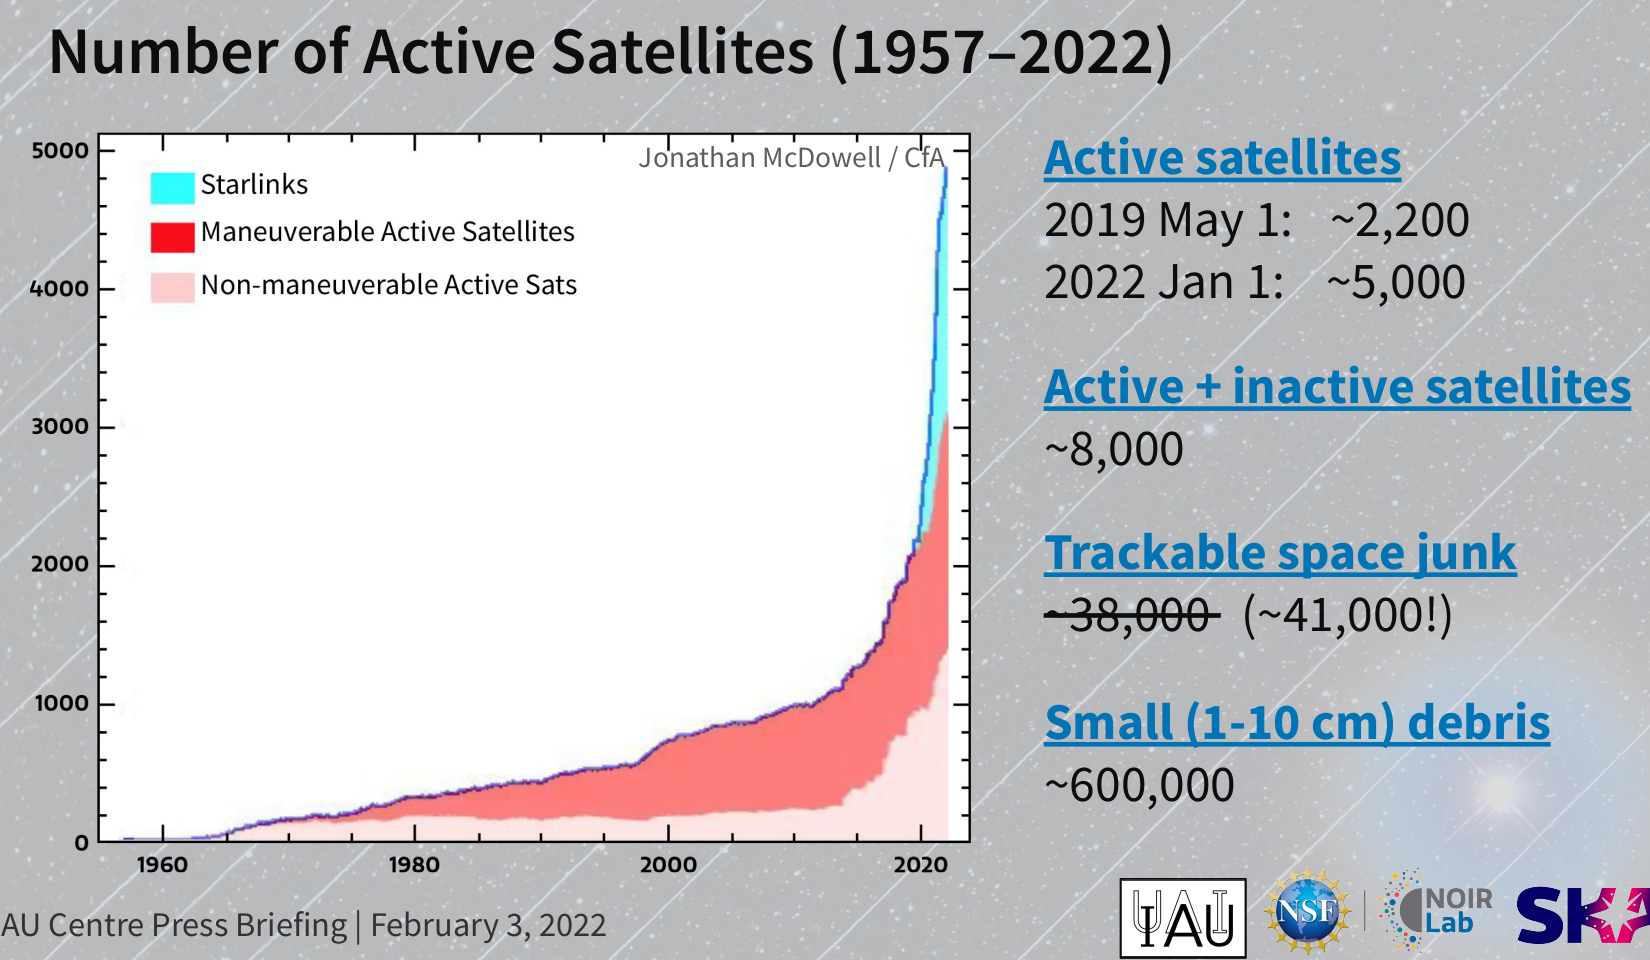
\includegraphics[width=0.8\linewidth]{ActiveSatellites}}
		  \centering \caption{\centering \tiny IAU Press}
	\end{minipage}
\end{figure}
	
\end{itemize}

%\end{itemize}


\note[item]{


\begin{itemize}
	
	\item Lehenik, Europako eta EEBBko plan teknologikoei erreferentzia eginez, gure ikerketaren errelebantzia nabarmendu nahiko nuke
	
	\medskip
	\item Gaur-egun satelite artifizialen garrantzia ukaezina da eta  azpimarratzekoa, azken urteetan izandako gorakada:	irudiko grafikoaren datuei erreparatuz: 2019. urteko satelite aktiboen kopurua (2.200),  2022.urtean biokiztu (5.000) egin da

	
	
	\medskip
	\item
%	 Euskadiko eta Estatuko Zientzia Planek  
    Europatik, sateliteen teknologiek  babes handia jasotzen dute eta   Horizon Europa estrategian bi helburu nagusi finkatzen dira: % zera jasotzen du:
	
	\medskip
	
	\begin{itemize}

	\item Espazioaren zaintza eta segurtasuna %ikerkuntza bultzatzea
	
	\medskip
	\item Europaren independentzia teknologikoa bermatzea %, bere teknologia garatzea

   \end{itemize}
	
	\medskip
	\item Aipatzekoa da ere, EEBBetako 2012.go Espazio teknologiaren ebaluazio  txostenean jasotakoa:  etorkizunean orbita propagaile eraginkorren garapena kritikoa izango dela eta hauek, konputazio paraleloan oinarritutako izan behar direla ondorioztatzen du


\end{itemize}



}


\end{frame}






%%%%%%%%%%%%%%%%%%%%%%%%%%%%%%%%%%%%%%%%%%%%%%%%%%%%%%%%%%%%%%%%%%%%%%%%%%%%%%%

\begin{frame}{2) Ikerketa proiektuaren balorazioa} 	

%\medskip

%\small
%\begin{itemize}
%\item Europako Parlamentuaren 541/2014/EE erabakia (SST proiektuak)
%
%\begin{itemize}
%\item Software librea bultzatzea
%\item Erabilpen segurua ziurtatzeko, \textbf{Software libreko} garapenak
%\end{itemize}

\textcolor{blue}{2.2) Software librea eta Julia}

\medskip
\begin{itemize}

\medskip
%\item Zergatik \textbf{Software librea}?
%

\item Zergatik \textbf{Julia}?
%
\medskip
\begin{itemize}
%	\item Software librea
	
%	\medskip
	\item Konputazio zientifikorako goi-mailako  lengoaia
	
%	\medskip
%	\item Goi-mailako lengoaia  
	
	\medskip
	\item Azkarra (C lengoaia bezain eraginkorra izan daiteke) 
	
	\medskip
	\item Konputazio paraleloa modu errazean
	
		\medskip
	\item Notebook dokumentu dinamikoak 
	
\end{itemize}
%\end{itemize}

\bigskip

\item \textbf{Software libreko} proiektuaren partaide izatearen abantailak:

\medskip

\begin{itemize}
%	\item Zientzia irekia

    \item Berrikuntzen leiho bat %: tresnak, arloak, $\dots$
    	
	\medskip
	\item Konputazio teknika aurreratuak
	%
	\medskip
	\item Ekarpenak egitea errazten da  
	
\end{itemize}


\begin{figure}
%
%
\begin{minipage}{.4\textwidth}
	\colorbox{white}  {
\includegraphics[width=0.8\linewidth]{SoftwareLibre}}
\end{minipage}
%
\begin{minipage}{.4\textwidth}
\colorbox{white}  {
\includegraphics[width=0.5\linewidth]{julia-logo-color}}
\end{minipage}
%

%
\end{figure}


\end{itemize}


\note{



\begin{itemize}


    \item  $2018.$ urtean gure garapenetarako Julia lengoai berria aukeratu genuen eta erabaki honek gure ikerketan eragin positiboa izan du. 


\item Julia?

\begin{itemize}
%	\item Software librea delako
	
	\medskip
	\item Konputazio zientifikorako goi-mailako lengoaia delako %, gure iritziz ondo diseinatua
	
	\medskip
	\item Azkarra da (C lengoaia bezain eraginkorra izan daiteke) 
	
	\medskip
	\item Konputazio paraleloa erraza
	
	\medskip
	\item Notebook dokumentu dinamikoak onartzen ditu

\end{itemize}

    \medskip
\item  Honek, software libreko proiektu honen partaide izatera eraman gaitu eta honek aldi berean hainbat  abantaila ekarri dizkigu:

\begin{itemize}
	
%	\item Zientzia irekiaren filosofiarekin bete-betean bat egiten du
	\item Guretzako berrikuntzen leiho bat da
	
	\medskip
	\item Konputazio teknika berriak ezagutzen eta aplikatzen laguntzen digu
	
	\medskip
	\item Ekarpenak egitea errazten da, eta zentzu horretan gure inplementazioa EDA-en ebazpenerako sisteman integratzea lortu dugu
%	Gure lanak ezagutarazteko bideak irekitzen dizkigu. Konkretuki, gure ustez ekuazio-diferentzialen software ekosistema onenean gure inplementazioak argitaratzeko aukera eman digu
	
\end{itemize}

\end{itemize}

}

\end{frame}




%%%%%%%%%%%%%%%%%%%%%%%%%%%%%%%%%%%%%%%%%%%%%%%%%%%%%%%%%%%%%%%%%%%%%%%%%%%%%%%

\begin{frame}{2) Ikerketa proiektuaren balorazioa}
		

	
\medskip

%4) 	


\textcolor{blue}{2.3)  Gradu eta Masterreko irakaskuntzari ekarpenak}
 

\bigskip

%Ikerketa-jarduerak, gradu eta masterreko \textbf{irakaskuntzak aberasteko} txerta daitezkeen alderdi asko ditu:

%\medskip



\begin{columns}

\column{0.5\textwidth}


\begin{itemize}
		
\item[1)] Modelizazioa

\medskip

\item[2)] Matematika

\medskip

\item[3)] Zenbakizko metodoak

\medskip

\item[4)] Programazioa

	
\end{itemize}


\column{0.2\textwidth}


\vspace*{1.cm}
\Large
$\Rightarrow$

\column{0.3\textwidth}

\vspace*{0.8cm}
%Irakasgaiekin erlazionatutako adibideak eta jarduerak
\textbf{Irakaskuntza aberastu}

\end{columns}

\note{


\begin{itemize}


\item Gure ikerketak gradu eta masterreko irakaskuntzari egin diezaizkioken ekarpenen inguruan esan,

%\medskip
%\item Ikerketak, gradu eta masterreko irakaskuntzak aberasteko txerta daitezkeen alderdi asko ditu:

\medskip
\item Gure ikerketan modelizazioa, matematika, zenbakizko meotodoak eta programazioa  konbinatzen ditugunez, modu naturalean irakagaiei erlazionatutako adibideak eta jarduerak sortzen zaizkigula.



\end{itemize}


}


\end{frame}

%%%%%%%%%%%%%%%%%%%%%%%%%%%%%%%%%%%%%%%%%%%%%%%%%%%%%%%%%%%%%%%%%%%%%%%%%%%%%%%

\begin{frame}{Ikerketa proiektua} 	
	
\medskip
\small
	
%\textcolor{blue}{Laburpena}: \textbf{Ikerketa proiektu}
%\bigskip

\Laburpena{Ikerketa proiektua}
{

\begin{itemize}
	
	\item[1)] \textbf{Ikerketa }: EDAk modelizatutako problemen zenbakizko integraziorako metodo aurreratuen analisia eta inplementazioa.
	
	
	\medskip
	
	\item[2)] \textbf{Etorkizuneko proiektuak}:
	%
    \begin{itemize}
    	\item Orain arteko gaietan sakondu
    	\medskip
    	\item Aplikazio berriak
    \end{itemize}
	
%	Konputagailuen \textbf{hardwarea esplotatzea} inplementazio eraginkorrak lortzeko
	
%	\medskip
	
	\item[3)] \textbf{Ikerketa proiektuaren balorazioa} 
	
	\begin{itemize}
		\item Zientzia eta teknologia planekin lerrokatzea
		\item Software librea eta Julia % proiektu batean parte-hartzearen abantailak
		\item Gradu eta Masterreko irakaskuntzari ekarpenak
	\end{itemize}
	
\end{itemize}

}

\note{


Ikerketa proiektuaren laburpen moduan,

\begin{itemize}
\item  Ikerketa, EDAk modelizatutako problemen zenbakizko integraziorako metodo aurreratuen analisian eta implementazioan, kokatzen dela.

Nabarmenduz,
\begin{itemize}
	\item Ekuazio diferentzialak,  zientzia eta ingeniaritza arloetako eredu ohikoena eta garrantzitsuena da. 
	
	\medskip
	\item Gehien bat N-gorputzetako probleman zentratu gara (oso aberatsa baita) 
	
	\medskip
	\item Gauss-en metodo inplizituen abantailak erakutsi nahi dugu 
	
	Metodo hauek \textbf{propietate konputazional eta matematiko} interesgarriak dituzte eta inplementazio bide berriak irekitzen dizkigu
	
	
\end{itemize}


\medskip

\item Etorkizuneko proiektuak

\medskip

Orain arte egindako lanari jarraipen naturala ematen dioten proiektuak direla

\medskip
\item Ikerketaren alde garrantzitsuak

\begin{itemize}
	\item Batez ere, sateliteen propagaziorako metodoei dagokionez, Europako zientzia planetN jasotzen den lehentasun bat da
	
	\medskip
	\item Software librea eta Julia. Azpimarratuz proiektu batean parte-hartzearen abantailak aipatu ditugu
	
	
	\medskip
	\item Gradu eta Masterreko irakaskuntza aberasteko edukiak sortzen zaizkigu
	
\end{itemize}

\end{itemize}


}



\end{frame}

%%%%%%%%%%%%%%%%%%%%%%%%%%%%%%%%%%%%%%%%%%%%%%%%%%%%%%%%%%%%%%%%%%%%%%%%%%%%%%%

%\begin{frame}{Garapen tresnak: Software librea}  	

%\bigskip
%\begin{itemize}
%\item  \textbf{Julia} programazio lengoaia

%\begin{itemize}
%\item \textit{J.H. Wilkinson Prize for Numerical Software 2019}
%\item \textbf{Open source}
%\item Konputazio zientifikoa % \textbf{computación científica}
%\item \textbf{Konputazio paraleloa}
%\end{itemize}

%\medskip
%\item \textbf{Jupyter}
%
%Testua, kodea eta irudiak konbinatzen dituzten dokumentuak sortzeko aukera ematen duen web interfazea


%Interfaz web que permite crear documentos donde se combinan texto, código y visualizaciones 
%

%\medskip
%\item \textbf{GitHub}
%
%Proiektuen biltegia (bertsioen kontrola)


%\end{itemize}

%\begin{figure}
%\begin{minipage}{0.4\textwidth}
%  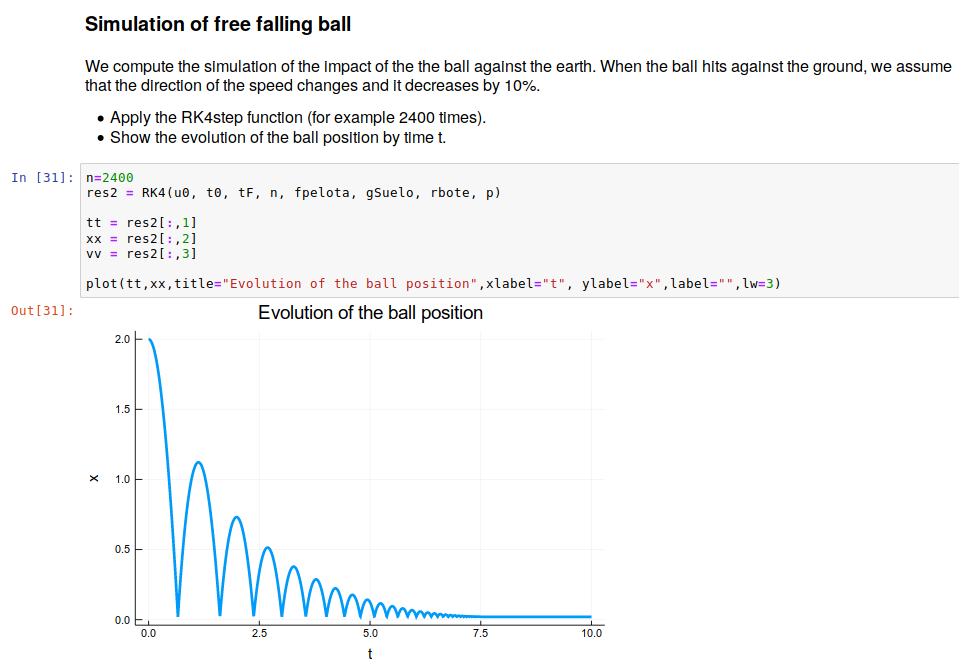
\includegraphics[width=0.8\linewidth]{JupyterAdba2}
%\end{minipage}
%
%\begin{minipage}{0.4\textwidth}
%  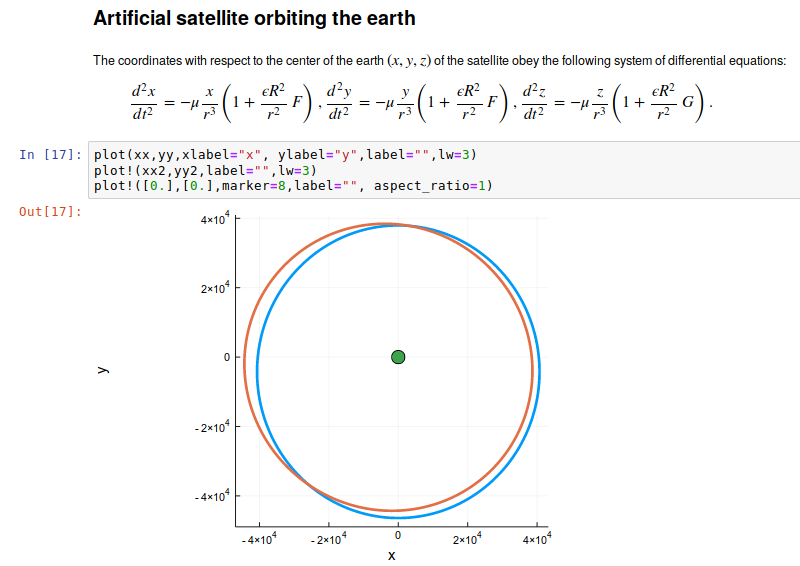
\includegraphics[width=0.8\linewidth]{JupyterAdba}
%\end{minipage}
%\hfill
%\end{figure}

%\end{frame} 


%%%%%%%%%%%%%%%%%%%%%%%%%%%%%%%%%%%%%%%%%%%%%%%%%%%%%%%%%%%%%%%%%%%%%%%%%%%%%%%
\section[Irakaskuntza programa (Aljebra)] {Irakaskuntza programa (Aljebra)}

\begin{frame}{Irakaskuntza programa (Aljebra)} 
	
%\medskip
	
  \tableofcontents[currentsection,currentsubsection]

\begin{figure}
	\begin{minipage}{1.\textwidth}
		\colorbox{white}  
%{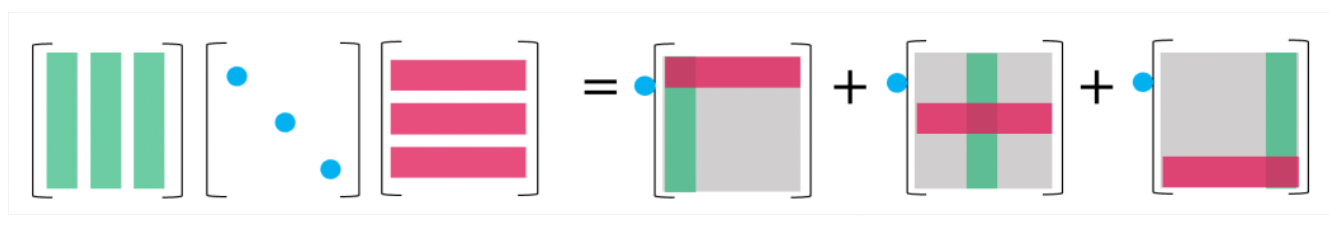
\includegraphics[width=1.\linewidth]{Irakaskuntza_Programa}}		
		{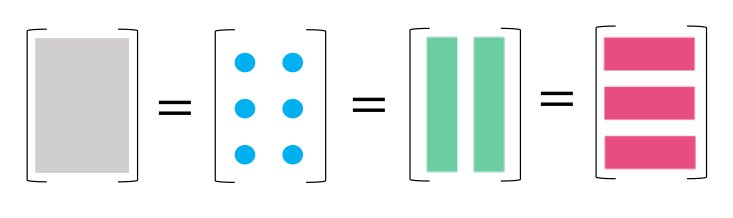
\includegraphics[width=1.\linewidth]{Matrix4Ways}}
		\centering \caption{\centering \tiny Matrize bat irudikatzeko 4 modu (The Art of Linear Algebra)}
	\end{minipage}
\end{figure}


\end{frame}


\note{


\begin{itemize}
	
	\medskip
	\item Aurkezpenaren azken zatira iritsita irakaskuntza programa aurkeztuko dut, eta nire kasuan,  Aljebra irakasgaia aukeratu dut
	
%	\medskip
%	\item Aljebra irakasgaiaren irakaskuntza programa azalduko dut
\end{itemize}





}



%%%%%%%%%%%%%%%%%%%%%%%%%%%%%%%%%%%%%%%%%%%%%%%%%%%%%%%%%%%%%%%%%%%%%%%%%%%%%%%

\begin{frame}{Irakaskuntza programa (Aljebra)} 
	
%	\medskip
	
	\hspace*{1.cm} \textcolor{red}{Zergatik Aljebra?} \hspace*{1.2cm} $\boldsymbol{\Rightarrow}$ \hspace*{1.2cm} \textcolor{blue}{Ikasleentzat erakargarria}
	
	\bigskip
	\small
	
	\begin{itemize}
		\item[1)] \textbf{Garrantzitsua} %: Egungo arlo garrantzitsuetan aplikatzen da:
		%
		\medskip
		\begin{itemize}
			\item Datu-analisia eta ikasketa automatikoa
			%
%			\item Ikasketa automatikoa
		\end{itemize}
		%
		
		\bigskip
		
		\item[2)] \textbf{Edukien azalpen aberatsa} %\hspace*{1.2cm} $\boldsymbol{\Rightarrow}$ \hspace*{1.2cm} \textcolor{red}{Ikasleentzat erakargarria}

%		
		\begin{figure}
			%
			\centering
			\begin{minipage}{.9\textwidth}
				\colorbox{white}  {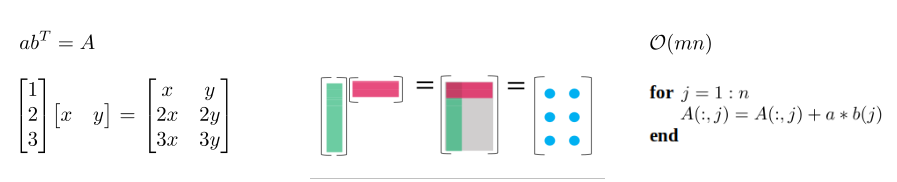
\includegraphics[width=0.9\linewidth]{Definizio bisualak3}}
			\end{minipage}
			%
		\end{figure}
	

		
		%   \medskip
		\item[3)] \textbf{Aplikazio interesgarriak klasean}
		%
		\begin{figure}
			%
			\centering
			\begin{minipage}{.3\textwidth}
%				\colorbox{white}  {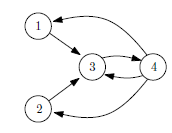
\includegraphics[width=0.8\linewidth]{sarea}}
				\colorbox{white}  {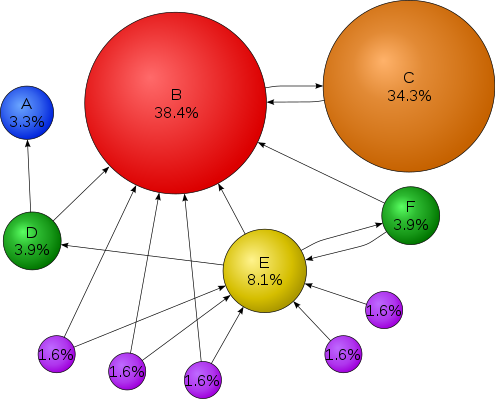
\includegraphics[width=0.6\linewidth]{PageRanks-Example-svg.png}}  \centering \caption{\centering \tiny Page-Rank (Wikipedia)}	
			\end{minipage}
			%
			\hfill
			\begin{minipage}{.3\textwidth}
				\colorbox{white}  {\includegraphics[width=0.8\linewidth]{Transformazio_linealak}}
				 \centering \caption{\centering \tiny Grafiko transformazioak (Strang)}
			\end{minipage}	
			%
			\hfill
			\begin{minipage}{.3\textwidth}
				\colorbox{white}  {\includegraphics[width=0.8\linewidth]{IrudiKonprimitzea}}
		    	 \centering \caption{\centering \tiny Irudien prozesamendua}
			\end{minipage}
		\end{figure}
		
		
		
	\end{itemize}


   \note{
   

\begin{itemize}
	\item Egungo arlo garrantzitsuetan aplikatzen delako
	
	
	\begin{itemize}
		\item     Datuen-analisia arloaren erdigunean dago:  datuak askotan matrize batean jasoko ditugu 
		
		\item 	Ikasketa-automatikoa. Aljebrak, optimizazio eta estatisikarekin batera paper nagusia jokatzen du
	\end{itemize}
	

    \medskip
    \item Aljebraren edukiak modu  aberatsean landu daitezke 
    
    \medskip
    Hau da, Aljebraren lengoai formala izanik, definizio formalak, modu ezberdinetan lagun daiteke:  adibideen bidez, definizio bisualak emanez, algoritmoen bidez,...

   \medskip
   \item 	Hainbat dira aljebran oinarritutako klasean landu daitezkeen aplikazio interesgarriak: 
	
	\begin{itemize}
		\item Google-en Page-rank problema, non, webgune sare baten estekak aztertuz webgune “garrantzitsuena” determinatzea
		
		\item Grafikoen transformazioak,  matrizeen biderkaduren bidez ikustea
		
		\item Irudiak zenbakien matrizeak direnez,  irudien prozesamendurako aplikazioak lantzea.
%		      Irudien konpresioa: balio singularren deskonposaketaren aplikazio
	\end{itemize}
	
	
	\item  Guzti honengatik, ikasleentzat erakargarria izan daitekeela iruditzen zait
	
\end{itemize}






}
	
	
\end{frame}


%%%%%%%%%%%%%%%%%%%%%%%%%%%%%%%%%%%%%%%%%%%%%%%%%%%%%%%%%%%%%%%%%%%%%%%%%%%%%%%
%\section[Irakaskuntzako programa (Aljebra)] {Irakaskuntzako programa (Aljebra)}

\begin{frame}{Irakaskuntza programa (Aljebra)} 

\medskip
\small



\begin{align*}
%
\begin{cases}
\text{UPV/EHUren hezkuntza-eredua} \\
\text{Informatika fakultateko bi graduak} \\
\text{Irakasgaiaren bibliografia}
\end{cases}
%
\quad \Rightarrow \quad 
\text{Aljebra programa}
%
\end{align*}


%
\bigskip


\begin{figure}
%
\begin{minipage}{.3\textwidth}
\colorbox{white}  {\includegraphics[width=0.8\linewidth]{IKDi3}}
\end{minipage}
%
\begin{minipage}{.3\textwidth}
\colorbox{white}  {\includegraphics[width=0.8\linewidth]{Adimen Artifiziala}}
\end{minipage}
%
\begin{minipage}{.3\textwidth}
\colorbox{white}  {\includegraphics[width=0.8\linewidth]{ProgAlgebra}}
\end{minipage}
%
\end{figure}


%\MarkoGorria{Nire ekarpenak}
%{

%\begin{itemize}
%	\item Edukiak: balio singularren deskonposaketa
%	\item Pedagogikoki:  
%\end{itemize}


%}


\note{

\begin{itemize}
	\item  Aljebra irakasgaiaren programa diseinatzeko, 
\begin{itemize}
	\item EHUko hezkuntza eredua
	\item Fakultateko bi graduen ikuspegi orokorra (informatikaren ingeniaritzko gradua, adimen artifizialeko gradua) 
	\item Irakasgaiaren bibliografia unibertsitateen programak
\end{itemize}
aztertu ditut

\item Irakasgaiaren diseinu on bat: edukiak (metodologiak baino gehiago)

\end{itemize}


}


\end{frame}


%%%%%%%%%%%%%%%%%%%%%%%%%%%%%%%%%%%%%%%%%%%%%%%%%%%%%%%%%%%%%%%%%%%%%%%%%%%%%%%

\begin{frame}{UPV/EHU-ren hezkuntza-eredua} 

\medskip
\small

\begin{itemize}
	
\item \textbf{UPV/EHUko Plan Estrategikoa 2022-2025}

\medskip

\item \textbf{IKD eredua (2010)}: Irakaskuntza Kooperatibo eta Dinamikoa


%\begin{itemize}
%\item[1)] Irakasleek ikasgelan berrikuntza eta IKT tresnak erabiltzea
%
%\item[2)] Ikasleak ikaskuntzako eragile aktibo
%\end{itemize}

\medskip
\item \textbf{IKD i3 estrategia (2019)}: Ikaskuntza x ikerkuntza x iraunkortasuna


\medskip

\item \textbf{Zeharkako Gaitasunen Katalogoa} (2019)


\bigskip

\item \textcolor{blue}{UPV/EHU-ren argazki bat}

\medskip
\begin{figure}
\centering
%
\begin{minipage}{.8\textwidth}
	\colorbox{white}  {\includegraphics[width=0.8\linewidth]{EHU_Datuetan}}
	%  \centering \caption{\centering \tiny wikipedia}
\end{minipage}
%
%	\begin{minipage}{.4\textwidth}
%		\colorbox{white}  {\includegraphics[width=0.8\linewidth]{ZeharkakoGaitasunak}}
		%  \centering \caption{\centering \tiny wikipedia}
%	\end{minipage}
\end{figure}


%\medskip
%\item \textbf{Alineamiento} con el resto de asignaturas de la titulación
%\begin{itemize}
%\item Contenidos
%\item Sistemas de aprendizajes
%\item Evaluación
%\end{itemize} 

%\medskip
%\item \textbf{Coherencia} entre objetivos,  actividades y evaluación  

%(periódicamente revisado)


%\medskip
%\item Enseñanza \textbf{basada en problemas}

%\medskip
%\item Aprendizaje \textbf{activo y constructivo}

%Sintetizar, diseñar, ofrecer soluciones, aportar análisis, actitud crítica 

%\item Remarcar la esencia sobre la rutina y práctica
\end{itemize}


\note{



\begin{itemize}
	
	\item Ondorengoak dira, UPV/EHU-ren hezkuntza eredua definitzen duten dokumentu nagusiak
%	\item UPV/EHUko Plan Estrategikoa 2022-2025
	
%	\medskip
%	\item 2010ean irakaskuntza kooperatiboa eta dinamikoa bultzatzen duen eredua onartu zen
	
%	\medskip
%	\item Ondoren 2019, urtean bi eguneraketa izan ditu
	
%	\begin{itemize}
%	\medskip
%	\item Egungo orientazio pedagokioetara egokitzeko, ereduaren berrirakurketa bat egin da 
%	\medskip
%	\item UPV/ EHUren Gaitasun Orokorren Katalogoaren (2019) argitalpena
%	\end{itemize}

    \item Dokumentu hauek aztertzeaz gain, UPV/EHU-ren argazki bat osatzeko, azpiko  datuak kontutan hartzea interesgarrua iruditu zait. %Aurreko estrategietan bultzaten diren helburu batzuk, zein egoeran dauden erakusten baitituzte:
    
    \begin{itemize}
    	\item Nabarmentzekoa 2023-2024 107 gradu eskaintza 
    	\item Ingelesez: hastapenean
    	\item Gradu bikoitzak eta formakuntza duala modalitatean: zifra garrantzitsuak
    \end{itemize}   
	
\end{itemize}


}

\end{frame}



%%%%%%%%%%%%%%%%%%%%%%%%%%%%%%%%%%%%%%%%%%%%%%%%%%%%%%%%%%%%%%%%%%%%%%%%%%%%%%%

%\begin{frame}{Visión general} 

%\medskip
%\textbf{Grados} impartidos en EIG de Gipuzkoa:
%
%\begin{itemize}
%\medskip
%\item  Grado en Ingeniería de Energías Renovables (Eibar)
%\medskip
%\item  Grado en Arquitectura Técnica
%\medskip
%\item  Grado en Ingeniería Civil 
%\medskip
%\item Ingenierias Industriales
%
%\medskip
%\begin{itemize}
%\item Grado en Ingeniería Eléctrica
%\item Grado en Ingeniería Electrónica Industrial y Automática
%\item Grado en Ingeniería Mecánica
%\item Doble Grado en Ing. Mecánica e Ing. Electrónica Industrial y Automática
%\end{itemize}
%\end{itemize}

%\end{frame}


%%%%%%%%%%%%%%%%%%%%%%%%%%%%%%%%%%%%%%%%%%%%%%%%%%%%%%%%%%%%%%%%%%%%%%%%%%%%%%%

\begin{frame}{KZAA Sailaren irakaskuntza} 
	
\medskip


\hspace*{3.cm} \textcolor{blue}{Informatika fakultatea}


\bigskip
\small

\begin{columns}
	\column{0.5\textwidth}
	\centering \textbf{Sailak}
	
	\medskip
	\begin{itemize}
		\item Konputagailuen Arkitektura eta Teknologia
		\item Konputazio Zientzia eta Adimen Artifiziala
		\item Lengoaia eta Sistema Informatikoak
	\end{itemize}
%
	\column{0.5\textwidth}
	\centering \textbf{Graduak}
	
	\medskip
	\begin{itemize}
		\item Informatika Ingeniaritzako Gradua
		\item Adimen Artifizialeko Gradua
	\end{itemize}
	
	
\end{columns}


\note{

Informatika fakultateko laburpen moduan, esan,

\medskip

\begin{itemize}
	\item Fakultatean hiru sail daude
		\begin{itemize}
		\item Konputagailuen Arkitektura eta Teknologia
		\item Konputazio Zientzia eta Adimen Artifiziala
		\item Lengoaia eta Sistema Informatikoak
	\end{itemize}

\medskip
	\item Bi gradu eskaintzen dira
	
	\medskip
	\begin{itemize}
		\item Informatika Ingeniaritzako Gradua
		\item Adimen Artifizialeko Gradua
	\end{itemize}
	
\end{itemize}



}


\end{frame}

%%%%%%%%%%%%%%%%%%%%%%%%%%%%%%%%%%%%%%%%%%%%%%%%%%%%%%%%%%%%%%%%%%%%%%%%%%%%%%%

\begin{frame}{KZAA Sailaren irakaskuntza} 

\medskip


\centering \color{red}  Aljebraren garrantzia graduan?

\medskip
\small

\begin{itemize}

\item \textcolor{blue}{KZAA-ren  2022/23 ikasturterako irakasgaien zerrenda}


\medskip
\begin{figure}
	\quad
	\begin{minipage}{0.8\textwidth}
		\colorbox{white}  {\includegraphics[width=0.8\linewidth]{KZAA_Irakasgaiak}}
		%  \centering \caption{\centering \tiny wikipedia}
	\end{minipage}
\end{figure}

\end{itemize}

\note{


\begin{itemize} 

%\item KZAA Sailaren 2022/23 ikasturterako graduen irakasgaien azterketa komenigarri da

%\medskip
%\item Azterketa honek,  Aljebra linealaren ezagutza beste irakasgai batzuren garapenerako beharrezkoa dela erakusten du

\medskip


\item Hau da KZAA sailaren 2022/23 ikasturterako irakasgaien zerrenda

\item  Zerrenda honetako irakasgai gehienen garapenerako, Aljebra linealaren ezagutza beharrezkoa dela nabarmendu daiteke:


\begin{itemize}
	\item Matematika diskretua
	\item Ikaskuntza automatikoa
	\item Konputagailu bidezko Grafikoak
%	\item Datu Meatzaritza
	\item Estatistika metodo aurreratuak
\end{itemize}

\end{itemize}


}

\end{frame}




%%%%%%%%%%%%%%%%%%%%%%%%%%%%%%%%%%%%%%%%%%%%%%%%%%%%%%%%%%%%%%%%%%%%%%%%%%%%%%%

\begin{frame}{Irakaskuntza programa} 
	
	\medskip


\centering \textcolor{red}{Ikasgaiaren erreferentzi bibliografikoa?}

\medskip

\begin{align*}
\textcolor{blue}{Programa}
\ \Rightarrow \
%
\begin{cases}
\textcolor{blue}{Aljebra \ irakasteko \ modu \ berriak} \\
\textcolor{blue}{Bibliografia \ bilaketa} 
%\textcolor{blue}{Unibertsitateen \  programak}\\
\end{cases}
\end{align*} 

%\begin{itemize}
%	\item 	\textcolor{blue}{Bibliografia bilaketa}
	
%\medskip
 %   \item 	\textcolor{blue}{Aljebra irakasteko ideia berriak}
%\end{itemize}	
	
	\medskip

%\hspace*{1.cm} MIT  \hspace*{2.cm} Stanford \& UCLA \hspace*{1.6cm} Stanford
\begin{figure}
	\begin{minipage}{0.3\textwidth}
		\colorbox{white}  {\includegraphics[width=0.8\linewidth]{linearalgebra5}}
		  \centering \caption{\centering \tiny 2016 (5. edizioa)}
	\end{minipage}
	%
	\begin{minipage}{0.3\textwidth}
		\colorbox{white}  {\includegraphics[width=0.8\linewidth]{Intro_To_LA}}
		  \centering \caption{\centering \tiny 2018}
	\end{minipage}
    %	
	\begin{minipage}{0.3\textwidth}
		\colorbox{white}  {\includegraphics[width=0.8\linewidth]{Numerical_LA}}
		  \centering \caption{\centering \tiny 2021}
	\end{minipage}
	%

\end{figure}


\note{

\begin{itemize}
	\item Programa zehazteko: aljebra irakasteko modu berriak proposatzen duten bibliografiaren bilaketa bat burutu dut


	\medskip
	\item Bilaketaren emaitzen artean, hainbat unibertsitateetan erreferentziazko  den  G.Strang-en Introduction to Linear Algebra (2016. urteko 5.edizioa) liburu ezaguna aukeratu dut
	
%	 Nik programa disenatzeko, 2016an argitaratutako G.Strang-en liburuan (5.edizioan) oinarritu naiz: hainbat unibertsitateko erreferentziazko liburua
	
%	\medskip
%	\item Beste bi liburuak, osagarriak kontsideratu ditut
%	\item Introduction to Applied Linear Algebra.   Stephen Boyd (2018): Stanford eta UCLA unibertsitateak
	
%	\medskip
%	\item Numerical Linear Algebra with Julia (2021). 
%	Ordenagailu laborategiko erreferentzia

\item Aipagarria da liburu honek: bideo azalpenak, ariketak eta inplementazio interesgarriak biltzen dituen webgunea duela

\end{itemize}
%Nik programa disenatzeko, G.Strang-en liburua oinarri hartu dut eta beste biak, osagarrizko erreferentziak kontsideratu ditut.

}
	
	
\end{frame}


%%%%%%%%%%%%%%%%%%%%%%%%%%%%%%%%%%%%%%%%%%%%%%%%%%%%%%%%%%%%%%%%%%%%%%%%%%%%%%%
%\begin{frame}{Competencias}


%\medskip
%\begin{itemize}
%\item Competencias Básicas y Competencias Generales de la Titulación

%\begin{itemize}
%\item Competencias Básicas (CB)
%\item Competencias Generales de la Titulación (C)
%\end{itemize}

%\medskip
%\item Competencias Específicas de la Formación Básica (FB)

%\medskip
%\item Competencias Específicas de la Rama Común Informática (RI)

%\medskip
%\item Competencias Específicas de Especialidad

%\begin{itemize}
%\item Ingeniería de Computadores (IC)
%\item Computación (CC)
%\item Ingeniería del Software (IS)
%\end{itemize}

%\end{itemize}

%\end{frame}


%%%%%%%%%%%%%%%%%%%%%%%%%%%%%%%%%%%%%%%%%%%%%%%%%%%%%%%%%%%%%%%%%%%%%%%%%%%%%%%

%\begin{frame}{Irakaskuntza programa} 

%\medskip

%\begin{figure}
%\begin{minipage}{1.\textwidth}
%\colorbox{white}  {\includegraphics[width=1.\linewidth]{Five_Factorizations}}
%\end{minipage}
%\end{figure}

%\medskip
%\begin{tikzpicture}
%\node[red](dot1) at (1.0, 0) {\textbullet};
%\end{tikzpicture}  
%\quad \textcolor{red}{Modificaciones}
%\end{frame}

%%%%%%%%%%%%%%%%%%%%%%%%%%%%%%%%%%%%%%%%%%%%%%%%%%%%%%%%%%%%%%%%%%%%%%%%%%%%%%%

%\begin{frame}{Irakaskuntza programa} 


%\begin{itemize}
%\medskip
%\item Lehen maila

%\medskip
%\item Aljebra linealaren \textbf{sarrera} % al álgebra lineal

%\medskip
%\item Hizkuntza: Euskara eta Gaztelania
%\medskip
%\item Kreditu kopurua: 6

%Distribuidos de la siguiente manera:
%\medskip
%
%\footnotesize
%\begin{table} [h!]
%\centering
%\begin{tabular}{ l c c c r} 
% \hline \\
% \textbf{Irakaskuntza} &  \textbf{Ordu} & \textbf{Ordu} & \textbf{Totala} \\ 
%\textbf{Mota} &  \textbf{presentzialak} & \textbf{ez-presentzialak} & \textbf{} \\ 
%\hline 
% Magistrala        & $40$ & $60$ & \boldmath{$100$} \\
% Gelako P.         & $10$ & $30$ & \boldmath{$40$}  \\
% Laborategiko P.   & $10$ & $0$  & \boldmath{$10$}  \\ 
% \hline 
% \textbf{Totala}    & \boldmath{$60$}  & \boldmath{$90$} & \boldmath{$150$} \\  
%\end{tabular}
%\end{table}




%\medskip
%\item Gaur egun  \textbf{Aljebraren garrantzia} nabarmendu behar da
%
% Destacar la \textbf{importancia del álgebra} en la actualidad. 
%
%Junto con la probabilidad/estadística y la optimización, forman la base del \textbf{machine learning} 

%\medskip

%\small
%\item Competencias (Álgebra)

%\end{itemize}

%

%\end{frame}

%%%%%%%%%%%%%%%%%%%%%%%%%%%%%%%%%%%%%%%%%%%%%%%%%%%%%%%%%%%%%%%%%%%%%%%%%%%%%%%

%\begin{frame}{Gaitasunak}

%\medskip
%\small


%\begin{itemize}
%	\item Irakasgaiaren gidan jasotako gaitasunak:
%\medskip

%\tiny
%\begin{table}[h!]
%	\caption[] 
%	{\small{}
%	\label{tab:fp1}       %
%	\centering
%	{%
%		\begin{tabular}{ l l} 
%			\hline
%			\textbf{Gaitasun mota}               &  \\
%			           & $-14.39$  & $-5.75$ & $-5.64$ & $-5.64$ \\ 
%			\hline
%			\\
%			Oinarrizko Gaitasunak & OG1, OG2, OG3, OG4, OG5        \\
%			\cline{1-1}           &                                \\
%			Gaitasun Orokorrak    & T8, T9, T10                    \\ 
%			Oinarrizko Heziketaren Gaitasunak    & OH1, OH3        \\
%			\\  
%			\hline
%	\end{tabular}}
%\%end{table}



%
%*
%'Graduaren gaitasunak.pdf' fitxategian, item bakoitzaren azalpena dago

%

%\medskip
%\small
%\item Gakoetariko bat ikasleak \textbf{problemak ebazteko gaitasuna} edukitzea da:
%
%\begin{itemize}
%	\item Problema egoera berri bat izan behar du: ebazteko zein prozedura matematiko argi ez dakiguna, ebazpide anitzekoa, $\dots$
%	\item Graduko ikasgaietako bakoitzak gaitasun horiek lortzen lagunduko dio ikasleari
%	\item Lehenengo mailako ikasgaiek,   
%\end{itemize}


%\end{itemize}


%\end{frame}


%%%%%%%%%%%%%%%%%%%%%%%%%%%%%%%%%%%%%%%%%%%%%%%%%%%%%%%%%%%%%%%%%%%%%%%%%%%%%%%

\begin{frame}{Irakaskuntza programa}
	
	
	\medskip
	\small
	
	\begin{itemize}
		
		
		\item  \textbf{Programa} \hspace*{4.5cm}  \textbf{Matrizeen faktorizazioa}	  
%
%\medskip
%
\begin{columns}
	
	\column{0.6\textwidth}
	
	\begin{itemize}
		\item[1)] Bektoreak eta matrizeak
		\item[2)] Sistema linealen ebazpena
		\item[3)] Bektore-espazioak
		\item[4)] Ortogonalitatea
		\item[5)] Determinanteak
		\item[6)] Balio-propio eta bektore-propioak
		\item[7)] \textcolor{red}{Balio singularren deskonposaketa} $\color{red}\Leftarrow$
	\end{itemize}
	
	\column{0.4\textwidth}
	
	\begin{figure}
		%
		\centering
		\begin{minipage}{.9\textwidth}
			\colorbox{white}  {\includegraphics[width=0.9\linewidth]{Matrize_Deskonposaketa}}
		\end{minipage}
		%
	\end{figure}
	
	
	
	
\end{columns}


\bigskip
		
		\item \textbf{Lau problema}
		
		\medskip
		\begin{table} [h!]
			\centering
			\begin{tabular}{ l c l l } 
				Problema & Dimentsioa & Gaiak & Deskribapena \\	
				\hline 
				$Ax=b$ & $n \times n$ & 1-2  & Sistema linealak \\
				$Ax=b$ & $m \times n$ & 3-4  & Karratu minimoak \\
				$Ax=\lambda x$ & $n \times n$  & 5-6  &  Balio-propioak  \\
				\color{black}$Av=\sigma u$ & \color{black}$m \times n$  & \color{black}7  & \color{black} Balio singularrak \\ 
				\hline
			\end{tabular}
		\end{table}
		%
		\bigskip
		
		
		
		%\item \textbf{Planificación}
		%\medskip
		%\begin{itemize}
		%\item Dividir cada tema en \textbf{unidades didácticas}
		%\item Planificación \textbf{semanal}
		
		\ %end{itemize}
		
	\end{itemize}
	
	
	\note{
		
		\begin{itemize}
			
%			\medskip
			
%			\item Irakasgaiaren gidaren oinarriak ontzat hartuz, hau da, gaitasunak edo ikasketa helburuak,  zuzenean irakaskuntzako programa aurkezten dizuet.
			
%			\medskip
			\item Liburu honen edukietan oinarrituz, irakasgaiaren programa ondorengo 7 gaietan bana daiteke
			
			\medskip
			\item Modu baliokidean edukiak lau problemen ebazpenen ikuspegitik  edo matrizeen bost faktorizazioen ikuspegitik zehaztu daitezke %zehaztu daiteke
			
			\medskip
			\item Edozein kasutan nabarmendu, normalean lantzen ez den balio singularren deskonposaketa gehitzea proposatzen dudala
			
			%	\medskip
			%	\begin{itemize}
			%		\item n x n tamaineko ekuazio sistema linealen soluzioen ebazpena (Gauss-en metodoa)
			%
			%		\item Problema ez karratuak: ekuazioak > ezezagunak (edo alderantziz). Soluziorik ez duten m x n tamaineko sistemak eta  karratu minimoen zentzuan hurbilpen bat kalkulatuko dugun
			%
			%		\item Autobalio eta autobektoren sistemen ebazpena
			%
			%		\item \textcolor{red}{Balio singularren sistemen ebazpena}  $\color{red}\Leftarrow$
			
			%	\end{itemize} 
			
			%    \medskip
			%   \item Matrizeen faktorizazioa: Matrizeak matrize sinplegoen arteko biderdura gisa faktorizatzea. 
			
			
			
		\end{itemize}
		
		
		
	}
	
\end{frame}


%%%%%%%%%%%%%%%%%%%%%%%%%%%%%%%%%%%%%%%%%%%%%%%%%%%%%%%%%%%%%%%%%%%%%%%%%%%%%%%

\begin{frame}{Irakaskuntza programa}


\medskip



\centering \textcolor{red}{
Zergatik balio singularren deskonposaketa?}
%	¿Porqué añadir la Descomposición en valores singulares?}
%
\begin{align*}
A=U\Sigma V^T %, 
\end{align*}

\begin{itemize}
%\item ¿Porqué incluir la Descomposición en valores singulares?
%
%\medskip
%

%&A\begin{bmatrix}
% &  &\\
%v_1 & \dots & v_k\\
% & & 
%\end{bmatrix}=
%
%\begin{bmatrix}
% &  &\\
%u_1 & \dots & u_k\\
% & & 
%\end{bmatrix} 
%
%\begin{bmatrix}
%\sigma_1 &  &\\
% & \ddots & \\
% & & \sigma_k
%\end{bmatrix}\\
%& \sigma_1\geqslant \sigma_2 \geqslant \cdots \geqslant \sigma_k>0 \qquad \text{rank}(A)=k 
%\end{align*}
%
%\begin{itemize}
\item Diagonalizazioaren \textbf{hurrengo urrats naturala da}  % $A=X\Lambda X^{-1}$

%\medskip
%\begin{itemize}
%\item[1)] $A$ matrizea karratua izatea
%\item[2)] $A$ matrizea beti ez da diagonalizagarria
%\item[3)] Bektore-propioak askotan ez dira ortogonalak
%Frecuentemente los vectores propios no son ortogonales
%\end{itemize}
%
\medskip
\item \textbf{Datu-analisiaren funtsezko tresna}  %$\Rightarrow$ \textbf{Aplikazio interesgarriak}:

\medskip
%
%\begin{itemize}
%\item Datu-matrizearen funtsezko informazioa aukeratzea
%
%\begin{align*}
%& \sigma_1\geqslant \sigma_2 \geqslant \cdots \geqslant \sigma_k>0 \qquad \text{rank}(A)=k 
%\end{align*}
%
%PCA (estatistika), irudiak konprimitzea, \dots

\begin{itemize}
	\item Irudien prozesamendua %: irudiak konprimitzea, aurpegien errekonozimendua
	\item Estatistika: osagai nagusien analisia (PCA) 
\end{itemize}

%\end{itemize}


\begin{figure}
	\begin{minipage}{0.8\textwidth}
		\colorbox{white}  {\includegraphics[width=0.8\linewidth]{Face_Recognition}}
		  \centering \caption{\centering \tiny Learning the parts of objects by non-negative matrix factorization, (Nature, Lee and Seung, 1999)}
	\end{minipage}
\end{figure}


\end{itemize}
%\end{itemize}


\note{


\begin{itemize}
	\item Diagonalizazioari jarraipena ematen dion hurrengo urrats naturala da.
	
	\medskip
	\item Diagonalizazioaren hiru problemak konpontzen ditu: 
	
	\begin{itemize}
		\item $A$ matrizea karratua izatea
		\item $A$ matrizea beti ez da diagonalizagarria
		\item Bektore-propioak askotan ez dira ortogonalak
	\end{itemize}
	
	\medskip
	\item Datu-analisiaren funtsezko tresna delako eta horien adibideak:
	
	%
	\begin{itemize}
		\item Irudien prozesamenduaren arloan

\begin{itemize}
	\item Irudien konpresioa
	\item Aurpegien errekonozimendua
\end{itemize}		
		
%		\item Aurpegien errekonozimendua
		\item Estatistika arloan: Osagai nagusien analisia (PCA)
	\end{itemize}
\end{itemize}




}

\end{frame}


%%%%%%%%%%%%%%%%%%%%%%%%%%%%%%%%%%%%%%%%%%%%%%%%%%%%%%%%%%%%%%%%%%%%%%%%%%%%%%%

\begin{frame}{Laborategiko praktiken programa}
	
	%\medskip
	\small
	\begin{itemize}
		
		\item Sarrera
		\begin{itemize}

		\item[1)] Softwarearen sarrera
		%
		\medskip
		\item[2)] Bektoreak eta matrizeak  %$\qquad S^T=S$
		%
     	\end{itemize}
		
		\medskip
		
		\item Aplikazioak
		
		\begin{itemize}
		%
		\item[3)] Grafoak \quad 
		\begin{minipage}{.2\textwidth}
			\colorbox{white}  {\includegraphics[width=0.8\linewidth]{IncidentMatrix}}
		\end{minipage}
		%
%		eta transformazioak
%		\begin{minipage}{.3\textwidth}
%			\colorbox{white}  {\includegraphics[width=0.6\linewidth]{Transformazio_linealak}}
%		\end{minipage}
		
%		\medskip
		\item[4)] %Matrizearen eragiketen konplexutasun konputazionala
		
		Konplexutasun konputazionala
		%
		\begin{align*}
		Ax:  \ \mathcal{O}(n^2), \quad AB:
		 \ \mathcal{O}(n^3), \qquad n=10, \ 100, \ 500, \ 1000, \ 2000 
		\end{align*}
		
		 % $\qquad A=LU$ 
		
		%$Ax=b, \qquad \text{dim}(A)=n \times n$ 
		%
		%\medskip
		%\item[4)] Ekuazio sistema linealen ebazpena:  $\quad A=QR\ $ (Gram Schmidt)
		%
		
		%$Ax=b, \qquad \text{dim}(A)=m \times n, \quad m>n \quad \Rightarrow \quad  \text{min}\|b-A\hat{x}\|$ 
		
		%
		%Ortogonalidad $\qquad Q^TQ=QQ^T=\mathrm{\mathit{I}}$
		%
		%\medskip
		
		\item[5)] Matrize bakanak: $A \in \R^{m\times n}, \quad n_{nz} \ll mn$
		
%  Matrize karratuen diagonalizazioa $\quad A=X\Lambda X^{-1}$
		%
		\medskip
		\item[6)] Irudien konpresioa $\quad A=U\Sigma V^T$
		%
		
		%Aplikazioa: irudi baten konpresioa
		%
		\begin{figure}
			\quad
			\begin{minipage}{.7\textwidth}
				\colorbox{white}  {\includegraphics[width=0.7\linewidth]{ZientziAstea2}}
				%  \centering \caption{\centering \tiny wikipedia}
			\end{minipage}
		\end{figure}
		
	\end{itemize}


\end{itemize}
	

\note{

 
% Laborategien praktiken programarako, aljebrak saio interesgarriak egiteko aukera ematen dut:

  Laborategietarako $6$ saioko programa bat diseinatu dut:

\begin{itemize}
	
	

    \medskip
    \item Softwarearen eta bektore/matrize sarrera moduko bi saio egin ondoren, beste lau saioak aplikazioei eskeiniko nizkioke 
	
	\medskip
	\item %Hirugarren saioan,  grafoak  bat deskribatzen duen A inzidentzia-matrizearen erabilera edo/ta grafikoen transformazioak 
	Matrizeen bidezko Grafoen inplementazioari %edota grafikoen transformazioak
	
	
	\medskip
	\item Matrizeen eragiketen konplexutasun konputazionala experimentazioari
	
%		\begin{align*}
%Ax:  \ \mathcal{O}(n^2), \quad AB:
%\ \mathcal{O}(n^3), \qquad n=10, \ 100, \ 500, \ 1000, \ 2000 
%\end{align*}
    	
 %   	konklusioa: $10^6 \times 10^6$ sistema bat (memorian sartuko balitz), 25 aste bainon gehiago beharko lituzke
    	
    
    \medskip
    \item  Matrize bakanak
    
    
    % A matrizeak egitura berezia badu (orokorrean A bakana bada elementu gehienak zeroak), egitura hau aprobetxatuz konputazioak modu eraginkorragoan egin daitezke.
	
	Matrizeen egitura berezia aprobetxatuz konputazioak modu eraginkorrean egin daitezkeela ilustratzeko.
	
	\medskip
	\item Eta 6. saioan, irudien konpresiorako balio singularren aplikazioa
\end{itemize}

    
%Zein software? Julia egokia izan liteke:
%- Software libre
%- Goi-mailakoa
%- Jupyter modukoa dokumentuak (aplika daiteke) 



}


\end{frame}



%%%%%%%%%%%%%%%%%%%%%%%%%%%%%%%%%%%%%%%%%%%%%%%%%%%%%%%%%%%%%%%%%%%%%%%%%%%%%%%

%\begin{frame}{Irakaskuntza motak eta materialak}


%\medskip

%\begin{itemize}
%	\item \textbf{Irakaskuntza motak}


%\medskip
%\begin{itemize}
%\item \textcolor{blue}{Klase magistrala}: eduki teorikoak eta adibideak% + test galdera%($26$)}  

%
%\medskip
%\item \textcolor{blue}{Gelako praktikak}: ariketak + test motako galderak%($8$)} 
%

%\medskip
%\item \textcolor{blue}{Laborategiko praktikak}: software matematiko % ($6$)} 


%
%\medskip
%\item \textcolor{blue}{Ordutegi trinkoa} ($\approx 2$): Idatzizko azterketak
%
%\begin{itemize}
%	\item Idatzizko azterketak
%\end{itemize}
%\end{itemize}
%
%\bigskip
%\item \textbf{Materialak}

%\medskip
%\begin{itemize}
%	\item \textcolor{blue}{Laburpenak} (definizioak eta teoremak)
	
%	\medskip
%	\item \textcolor{blue}{Ariketa  bilduma} (emaitzekin)
	
%	\medskip
%	\item \textcolor{blue}{Test galderak}
	
%\end{itemize}

%\end{itemize}


%\note{

%Irakakuntza antolaketaren inguruan
%\begin{itemize}
%	\item Klase magistralak: Eduki teorikoen aurkezpena eta hauek ilustratzeko adibideak
	
%	test 
%	galdera: aukera anitzeko galderak, klasean eztabaida pizteko
    
%    \medskip
 %   \item Gelako praktikak: Ordu horietan ariketak egingo ditugu. 
 %   Taldeak txikiagoak direnez, eztabaida pizteko test-motako galdera egingo dira.
 
    
 %   \medskip
 %   \item Laborategiko praktikak. Aljebra linealaren problemak ebazteko Software matematiko batean trebatuko dira ikasleak
    
 %   \medskip
 %   \item Ordutegi trinkoko asteak, ebaluazio jarraituko idatzizko azterketak erabiliko ditugu
%\end{itemize}

 % Ikasleak e-gelan eskuragarri izango ditun materialak:
 %\begin{itemize}
 %	\item Definizioak eta teorema nagusien jasotzen dituen
% 	 dokumentua
 %	 \item Ariketa bilduma (emaitzekin)
 %	 \item Test galdera
 %\end{itemize}



%}

%\end{frame}


%%%%%%%%%%%%%%%%%%%%%%%%%%%%%%%%%%%%%%%%%%%%%%%%%%%%%%%%%%%%%%%%%%%%%%%%%%%%%%%

\begin{frame}{Irakaskuntza motak}


%\medskip
\small

\begin{itemize}


\item \textbf{Irakaskuntza motak}  

\begin{figure}
	
	\begin{minipage}{.9\textwidth}
		\colorbox{white}  {\includegraphics[width=0.9\linewidth]{Dedikazioa1}}
		%    			  \centering \caption{\centering \tiny Gorputzen arteko gerturatzeak}
	\end{minipage}
\end{figure}

\medskip

\item \textbf{Irakasgaiari dedikazioa}
%


\begin{figure}
%	
	\begin{minipage}{.7\textwidth}
		\colorbox{white}  {\includegraphics[width=0.7\linewidth]{Dedikazioa2}}
		%    			  \centering \caption{\centering \tiny Gorputzen arteko gerturatzeak}
	\end{minipage}
\end{figure}





\end{itemize}


\note{

Irakaskuntza gidan jasotzen den moduan  hiru dira irakaskuntza motak:
\begin{itemize}
	\item Klase Magistralak
	Eduki teorikoen aurkezpenerako 
	
	%eta hauek ilustratzeko adibideak
	Astero , 1:30 iraupeneko 2 saiorekin.
	
	\medskip
	\item Gelako praktikak
	
	Taldeak txikiagoak dira eta eztabaidarako/zalantzak argitzeko une egokiena da

%	Taldeak txikiagoak direnez, eztabaida pizteko test-motako galdera egingo dira.

	Bi astean behin 1:30 minituko saio bat
	
	\medskip
	\item Laborategiko praktikak
	
%	Aljebra linealaren problemak ebazteko Software matematiko batean trebatuko dira ikasleak
	Bi astean behin 1:30minuko saio bat
	
	
	\medskip
	\item 6 kreditoko ikasgaia den neurrian,
	
	Ikaslearen eskola ordutegitik kanpoko asteko dedikazioa	
	
	6 ordukoa izan behar  dela (ariketak, azterketarako ikasten,...) estimatzen da  
	
\end{itemize}



}

\end{frame}


%%%%%%%%%%%%%%%%%%%%%%%%%%%%%%%%%%%%%%%%%%%%%%%%%%%%%%%%%%%%%%%%%%%%%%%%%%%%%%%

%\begin{frame}{Adibidea: test galdera}

%El alumnado deberá elegir para ser evaluado entre dos sistemas:
%Evaluación formativa



%\begin{figure}
%\quad
%\begin{minipage}{.9\textwidth}
%\colorbox{white}  {\includegraphics[width=0.9\linewidth]{socrative-adba}}
%  \centering \caption{\centering \tiny wikipedia}
%\end{minipage}
%\end{figure}


%\note{


%\begin{itemize}
%	\item Ahozkotasuna lantzea
%	\item Klasean parte-hartzea eta eztabaida bultzatzea
%	\item Kontzeptuen ezagutza hobetzea
%\end{itemize}



%}

%\end{frame}


%%%%%%%%%%%%%%%%%%%%%%%%%%%%%%%%%%%%%%%%%%%%%%%%%%%%%%%%%%%%%%%%%%%%%%%%%%%%%%%

%\begin{frame}{Adibidea: test galdera}
	
	%El alumnado deberá elegir para ser evaluado entre dos sistemas:
	%Evaluación formativa
	
	
	
%	\begin{figure}
%		\quad
%		\begin{minipage}{.9\textwidth}
%			\colorbox{white}  {\includegraphics[width=0.9\linewidth]{socrative-adba2}}
			%  \centering \caption{\centering \tiny wikipedia}
%		\end{minipage}
%	\end{figure}
	
	
	
%\end{frame}



%%%%%%%%%%%%%%%%%%%%%%%%%%%%%%%%%%%%%%%%%%%%%%%%%%%%%%%%%%%%%%%%%%%%%%%%%%%%%%%

\begin{frame}{Ebaluazioa}
	

\medskip
%\small

\centering \textcolor{blue}{Ebaluazioa}

\medskip

\begin{figure}
	%
	\centering
	\begin{minipage}{.8\textwidth}
		\colorbox{white}  {\includegraphics[width=0.8\linewidth]{Kalifikazio_portzentaia}}
	\end{minipage}
	%
\end{figure}



\footnotesize
\begin{table} [h!]
	\centering
	\begin{tabular}{l l l l c} 
		\multicolumn{4}{c}{\textcolor{blue}{JARRAITUA}} & \textcolor{red}{FINALA} \\ \\
		\textcolor{blue}{Proba}  & \textcolor{blue}{Gaiak}         & \textcolor{blue}{Pisua}  &  \textcolor{blue}{Data} &  \\    
		\hline 
		1. Idatzizko azterketa       & 1,2            & $\%15$  & Martxoa &    \\
		2. Idatzizko azterketa       & 3,4            & $\%15$  & Apirila &   \\
		3. Idatzizko azterketa       & 1,2,3,4,5,6,7  & $\%30$  & Maiatza &  \textcolor{red}{X}  \\
	\end{tabular}
\end{table}



\note{
	
	
	Ebaluazioari dagokionez, ondorengo proposamena egingo nuke
	
	\medskip
	
	\begin{itemize}
		\item Kalifikazioak hiru zatitan banatuko nituzke:

	\begin{itemize}
		\item Idatzizko azterketak $\%60$ pisua	

		%
		\item Laborategiak: a $\%25$ pisua
		%
		\item Banakako lana: 
		
	\end{itemize}

       \item Eta zati bakoitza kalifikatzeko
       
    \begin{itemize}
   
	
	\item Ebaluazio jarraiturako
				idatzizko 3 proba, taulan azaltzen den antolaketarekin
%		\medskip
%		\item Finala
		%
%		\begin{itemize}
%			\item Idatzizko proba bakarra 
%			\item Laborategiko azterketa eta banakako lana egun berean
%		\end{itemize}


    \item Laborategia: azterketa proba batekin ebaluatuko litzateke et
    
    \item Banakako lana: lauhilekoan zehar klasean jasotako hainbat ariketa txikirekin ebaluatuko litzatekeena
    

    \end{itemize}
	
	\end{itemize}
	
	
}





\end{frame}
	
	
%%%%%%%%%%%%%%%%%%%%%%%%%%%%%%%%%%%%%%%%%%%%%%%%%%%%%%%%%%%%%%%%%%%%%%%%%%%%%%%

\begin{frame}{Irakaskuntza programa (Aljebra)}
	
	
\medskip
\small

\Laburpena{Irakaskuntza programa}
{


\medskip
\begin{itemize}
	\item Aljebra irakasteko modu berriak
	
	\medskip
	\item Introduction to Linear Algebra (G.Strang, 2016)
	
	\medskip
	\item Balio singularren deskonposaketa 


\medskip

\begin{figure}
	%
	\centering
	\begin{minipage}{.6\textwidth}
		\colorbox{white}  {\includegraphics[width=0.6\linewidth]{blacboards2}}
	    \centering \caption{\centering \tiny Do not erase}
	\end{minipage}
	%
\end{figure}
	 
\end{itemize}



}


\note{


\begin{itemize}
	\item Aljebra irakasteko modu berrien alde egingo nuke
	
	Frogapenetan oinarritutako estilotik aldenduz
	
	\medskip
	\item Erreferentziazko liburua Introduction to Lineal Algebra (G.Strang, 2016)
	
	\medskip
	\item Balio sigularren deskonposaketaren gaia landuko nuela
	
	
	
	
\end{itemize}



}

\end{frame}

%%%%%%%%%%%%%%%%%%%%%%%%%%%%%%%%%%%%%%%%%%%%%%%%%%%%%%%%%%%%%%%%%%%%%%%%%%%%%%%

%\begin{frame}{Ebaluazioa}

%El alumnado deberá elegir para ser evaluado entre dos sistemas:
%Evaluación formativa

%\begin{itemize}

%\item \textbf{Ebaluazio jarraitua} \small$\ \  \boxed{Nota=1+ 2+ 3}$

%\medskip
%Actividades que permitan valorar el progreso de cada estudiante 
%\begin{itemize}

%\small
%\medskip
%\item[1)] \textbf{Idatzizko probak} ($\%60$) 
%
%\medskip
%\footnotesize
%\begin{table} [h!]
%\centering
%\begin{tabular}{l l l l} 
%\textcolor{blue}{Proba}  & \textcolor{blue}{Gaiak}         & \textcolor{blue}{Pisua}  &  \textcolor{blue}{Data}  \\    
% \hline 
%1. Idatzizko proba       & 1,2            & $\%15$  & Martxoa    \\
%2. Idatzizko proba       & 3,4            & $\%15$  & Apirila    \\
%3. Idatzizko proba       & 1,2,3,4,5,6,7  & $\%30$  & Maiatza    \\
%\end{tabular}
%\end{table}

%\medskip
%\small
%\item[2)] \textbf{Laborategiko praktikak} ($\%25$):  azterketa proba bat 
%

%\medskip
%\item[3)] \textbf{Banakako lana} ($\%15$): test galderak 
%

%\end{itemize}

%\medskip

%\item \textbf{Ebaluazio globala} \small$\ \  \boxed{Nota=1+ 2+3}$

%\medskip
%\begin{itemize}
%\item[1)] \textbf{Idatzizko azterketa} ($\%60$) 
%\item[2)] \textbf{Laborategi ordenagailuen azterketa} ($\%25$)  
%\item[3)] \textbf{Ahozko azterketa} ($\%15$): test galderak 
%\end{itemize}

%\medskip

%\item \textcolor{red}{Ez-ohiko deialdia}: $2$ eta $3$ mantentzeko aukera emanez

%\end{itemize}


%\note{


%\begin{itemize}
%	\item Jarraitua
	
%	\medskip
%	\begin{itemize}
%		\item Idatziko 3 proba, $\%60$ pisuarekin eta taulan azaltzen den antolaketarekin
		%
%		\item Azterketa proba batekin ebaluatuko litzateke
		%
%		\item Banakako lana: lauhilekoan zehar test moduko 3 proben bidez
%	\end{itemize}

%    \medskip
%    \item Globala
    %
%    \begin{itemize}
%    	\item Idatzizko proba bakarra $\%75$ pisuarekin
%    	\item Laborategiko azterketa
%    \end{itemize}
%\end{itemize}



%}

%\end{frame}




%%%%%%%%%%%%%%%%%%%%%%%%%%%%%%%%%%%%%%%%%%%%%%%%%%%%%%%%%%%%%%%%%%%%%%%%%%%%%%%

%\begin{frame}{Bibliografía}

%\small
%\medskip

%\begin{itemize}
%	\item \textbf{Liburuak}

%\medskip

%\begin{figure}
%	\begin{minipage}{0.3\textwidth}
%		\colorbox{white}  {\includegraphics[width=0.8\linewidth]{linearalgebra5}}
		%  \centering \caption{\centering \tiny wikipedia}
%	\end{minipage}
	%
%	\begin{minipage}{0.3\textwidth}
%		\colorbox{white}  {\includegraphics[width=0.8\linewidth]{Intro_To_LA}}
		%  \centering \caption{\centering \tiny wikipedia}
%	\end{minipage}
	%	
%	\begin{minipage}{0.3\textwidth}
%		\colorbox{white}  {\includegraphics[width=0.8\linewidth]{Numerical_LA}}
		%  \centering \caption{\centering \tiny wikipedia}
%	\end{minipage}
	%
	
%\end{figure}

%\bigskip

%\medskip

%\item \textbf{Web errekurtsoak}: ariketak eta inplementazioak

%Solución a los problemas, ejercicios adicionales, implementaciones

%\medskip
%\begin{itemize}
%\item[1)] 
%\url{math.mit.edu/linearalgebra}

%\medskip
%\item[2)] \url{github.com/EricDarve/numerical_linear_algebra}

%\end{itemize}


%\end{itemize}

%\note{

%\begin{itemize}
%	\item Oinarrizko bibliografia, lehen aipatutako hiru liburuak gomendatuko nituzke
	
%	\medskip
%	\item Hauetako erreferentzi bakoitzak, ariketa eta inplementazio interesgarriak biltzen dituen
%	webgunea du
%\end{itemize}


%}

%\end{frame}



%%%%%%%%%%%%%%%%%%%%%%%%%%%%%%%%%%%%%%%%%%%%%%%%%%%%%%%%%%%%%%%%%%%%%%%%%%%%%%%

\begin{frame}

\bigskip
	

	
%	  \tableofcontents

\hspace*{2.cm} \Large \color{black}Eskerrik asko zuen arretagatik
%\huge \color{black} Gracias a tod@s 
\vskip 0.4cm

\begin{center}
         \includegraphics[width=.4\textwidth]{11-Semi-Axis-Earth}
\end{center} 



\vskip 0.2 cm

%\Large \color{blue}Eskerrikasko zuen arretagaitik
%\huge \color{black} Gracias a tod@s 
%\vskip 0.4cm

%\normalsize \color{black}mikel.antonana@ehu.eus



\centering \large \textcolor{blue}{mikel.antonana@ehu.eus}


\small
%\textcolor{red}{Aurkezpena helbide honetan eskuragarri}


%\begin{itemize}
%	\item Aurkepena:
%	\url{ https://github.com/mikelehu/Atxiki-Plaza-PAC8L2-D00140-8}
%\end{itemize}



\end{frame}


%\bibliography{./mybib}
% BibTeX users please use one of
%\bibliographystyle{spbasic}      % basic style, author-year citations
\bibliographystyle{spmpsci}      % mathematics and physical sciences
%\bibliographystyle{spphys}       % APS-like style for physics
\bibliography{bibliography}   % name your BibTeX data base

\end{document}





